              
                %% bare_jrnl.tex
%% V1.4b
%% 2015/08/26
%% by Michael Shell
%% see http://www.michaelshell.org/
%% for current contact information.
%%
%% This is a skeleton file demonstrating the use of IEEEtran.cls
%% (requires IEEEtran.cls version 1.8b or later) with an IEEE
%% journal paper.
%%
%% Support sites:
%% http://www.michaelshell.org/tex/ieeetran/
%% http://www.ctan.org/pkg/ieeetran
%% and
%% http://www.ieee.org/

%%*************************************************************************
%% Legal Notice:
%% This code is offered as-is without any warranty either expressed or
%% implied; without even the implied warranty of MERCHANTABILITY or
%% FITNESS FOR A PARTICULAR PURPOSE! 
%% User assumes all risk.
%% In no event shall the IEEE or any contributor to this code be liable for
%% any damages or losses, including, but not limited to, incidental,
%% consequential, or any other damages, resulting from the use or misuse
%% of any information contained here.
%%
%% All comments are the opinions of their respective authors and are not
%% necessarily endorsed by the IEEE.
%%
%% This work is distributed under the LaTeX Project Public License (LPPL)
%% ( http://www.latex-project.org/ ) version 1.3, and may be freely used,
%% distributed and modified. A copy of the LPPL, version 1.3, is included
%% in the base LaTeX documentation of all distributions of LaTeX released
%% 2003/12/01 or later.
%% Retain all contribution notices and credits.
%% ** Modified files should be clearly indicated as such, including  **
%% ** renaming them and changing author support contact information. **
%%*************************************************************************


% *** Authors should verify (and, if needed, correct) their LaTeX system  ***
% *** with the testflow diagnostic prior to trusting their LaTeX platform ***
% *** with production work. The IEEE's font choices and paper sizes can   ***
% *** trigger bugs that do not appear when using other class files.       ***                          ***
% The testflow support page is at:
% http://www.michaelshell.org/tex/testflow/


% Please refer to your journal's instructions for other
% options that should be set.
\documentclass[journal,onecolumn]{IEEEtran}
\makeatletter
\long\def\@makecaption#1#2{\ifx\@captype\@IEEEtablestring%
\footnotesize\begin{center}{\normalfont\footnotesize #1}\\
{\normalfont\footnotesize\scshape #2}\end{center}%
\@IEEEtablecaptionsepspace
\else
\@IEEEfigurecaptionsepspace
\setbox\@tempboxa\hbox{\normalfont\footnotesize {#1.}~~ #2}%
\ifdim \wd\@tempboxa >\hsize%
\setbox\@tempboxa\hbox{\normalfont\footnotesize {#1.}~~ }%
\parbox[t]{\hsize}{\normalfont\footnotesize \noindent\unhbox\@tempboxa#2}%
\else 
\hbox to\hsize{\normalfont\footnotesize\hfil\box\@tempboxa\hfil}\fi\fi}
\makeatother
%conference
% If IEEEtran.cls has not been installed into the LaTeX system files,
% manually specify the path to it like:
% \documentclass[journal]{../sty/IEEEtran}





% Some very useful LaTeX packages include:
% (uncomment the ones you want to load)


% *** MISC UTILITY PACKAGES ***
%
%\usepackage{ifpdf}
% Heiko Oberdiek's ifpdf.sty is very useful if you need conditional
% compilation based on whether the output is pdf or dvi.
% usage:
% \ifpdf
%   % pdf code
% \else
%   % dvi code
% \fi
% The latest version of ifpdf.sty can be obtained from:
% http://www.ctan.org/pkg/ifpdf
% Also, note that IEEEtran.cls V1.7 and later provides a builtin
% \ifCLASSINFOpdf conditional that works the same way.
% When switching from latex to pdflatex and vice-versa, the compiler may
% have to be run twice to clear warning/error messages.



% *** Custom Packages ***

%
\usepackage{booktabs}   % For professional table lines (\toprule, \midrule, \bottomrule)
\usepackage{tabularx}   % For tables that automatically fit the page width
% \usepackage{geometry}   % Recommended to manage page margins




% *** CITATION PACKAGES ***
%
\usepackage{cite}
% cite.sty was written by Donald Arseneau
% V1.6 and later of IEEEtran pre-defines the format of the cite.sty package
% \cite{} output to follow that of the IEEE. Loading the cite package will
% result in citation numbers being automatically sorted and properly
% "compressed/ranged". e.g., [1], [9], [2], [7], [5], [6] without using
% cite.sty will become [1], [2], [5]--[7], [9] using cite.sty. cite.sty's
% \cite will automatically add leading space, if needed. Use cite.sty's
% noadjust option (cite.sty V3.8 and later) if you want to turn this off
% such as if a citation ever needs to be enclosed in parenthesis.
% cite.sty is already installed on most LaTeX systems. Be sure and use
% version 5.0 (2009-03-20) and later if using hyperref.sty.
% The latest version can be obtained at:
% http://www.ctan.org/pkg/cite
% The documentation is contained in the cite.sty file itself.






% *** GRAPHICS RELATED PACKAGES ***
%
\ifCLASSINFOpdf
  \usepackage[pdftex]{graphicx}
  % declare the path(s) where your graphic files are
  \graphicspath{{./images/}}
  % and their extensions so you won't have to specify these with
  % every instance of \includegraphics
  \DeclareGraphicsExtensions{.pdf,.jpeg,.png}
\else
  % or other class option (dvipsone, dvipdf, if not using dvips). graphicx
  % will default to the driver specified in the system graphics.cfg if no
  % driver is specified.
  \usepackage[dvips]{graphicx}
  % declare the path(s) where your graphic files are
  \graphicspath{./images/}
  % and their extensions so you won't have to specify these with
  % every instance of \includegraphics
  \DeclareGraphicsExtensions{.eps}
\fi
% graphicx was written by David Carlisle and Sebastian Rahtz. It is
% required if you want graphics, photos, etc. graphicx.sty is already
% installed on most LaTeX systems. The latest version and documentation
% can be obtained at: 
% http://www.ctan.org/pkg/graphicx
% Another good source of documentation is "Using Imported Graphics in
% LaTeX2e" by Keith Reckdahl which can be found at:
% http://www.ctan.org/pkg/epslatex
%
% latex, and pdflatex in dvi mode, support graphics in encapsulated
% postscript (.eps) format. pdflatex in pdf mode supports graphics
% in .pdf, .jpeg, .png and .mps (metapost) formats. Users should ensure
% that all non-photo figures use a vector format (.eps, .pdf, .mps) and
% not a bitmapped formats (.jpeg, .png). The IEEE frowns on bitmapped formats
% which can result in "jaggedy"/blurry rendering of lines and letters as
% well as large increases in file sizes.
%
% You can find documentation about the pdfTeX application at:
% http://www.tug.org/applications/pdftex
\usepackage[caption=false, font=footnotesize]{subfig}




% *** MATH PACKAGES ***
%
%\usepackage{amsmath}
% A popular package from the American Mathematical Society that provides
% many useful and powerful commands for dealing with mathematics.
%
% Note that the amsmath package sets \interdisplaylinepenalty to 10000
% thus preventing page breaks from occurring within multiline equations. Use:
%\interdisplaylinepenalty=2500
% after loading amsmath to restore such page breaks as IEEEtran.cls normally
% does. amsmath.sty is already installed on most LaTeX systems. The latest
% version and documentation can be obtained at:
% http://www.ctan.org/pkg/amsmath





% *** SPECIALIZED LIST PACKAGES ***
%
%\usepackage{algorithmic}
% algorithmic.sty was written by Peter Williams and Rogerio Brito.
% This package provides an algorithmic environment fo describing algorithms.
% You can use the algorithmic environment in-text or within a figure
% environment to provide for a floating algorithm. Do NOT use the algorithm
% floating environment provided by algorithm.sty (by the same authors) or
% algorithm2e.sty (by Christophe Fiorio) as the IEEE does not use dedicated
% algorithm float types and packages that provide these will not provide
% correct IEEE style captions. The latest version and documentation of
% algorithmic.sty can be obtained at:
% http://www.ctan.org/pkg/algorithms
% Also of interest may be the (relatively newer and more customizable)
% algorithmicx.sty package by Szasz Janos:
% http://www.ctan.org/pkg/algorithmicx



% *** ALIGNMENT PACKAGES ***
%
%\usepackage{array}
% Frank Mittelbach's and David Carlisle's array.sty patches and improves
% the standard LaTeX2e array and tabular environments to provide better
% appearance and additional user controls. As the default LaTeX2e table
% generation code is lacking to the point of almost being broken with
% respect to the quality of the end results, all users are strongly
% advised to use an enhanced (at the very least that provided by array.sty)
% set of table tools. array.sty is already installed on most systems. The
% latest version and documentation can be obtained at:
% http://www.ctan.org/pkg/array


% IEEEtran contains the IEEEeqnarray family of commands that can be used to
% generate multiline equations as well as matrices, tables, etc., of high
% quality.




% *** SUBFIGURE PACKAGES ***
%\ifCLASSOPTIONcompsoc
%  \usepackage[caption=false,font=normalsize,labelfont=sf,textfont=sf]{subfig}
%\else
%  \usepackage[caption=false,font=footnotesize]{subfig}
%\fi
% subfig.sty, written by Steven Douglas Cochran, is the modern replacement
% for subfigure.sty, the latter of which is no longer maintained and is
% incompatible with some LaTeX packages including fixltx2e. However,
% subfig.sty requires and automatically loads Axel Sommerfeldt's caption.sty
% which will override IEEEtran.cls' handling of captions and this will result
% in non-IEEE style figure/table captions. To prevent this problem, be sure
% and invoke subfig.sty's "caption=false" package option (available since
% subfig.sty version 1.3, 2005/06/28) as this is will preserve IEEEtran.cls
% handling of captions.
% Note that the Computer Society format requires a larger sans serif font
% than the serif footnote size font used in traditional IEEE formatting
% and thus the need to invoke different subfig.sty package options depending
% on whether compsoc mode has been enabled.
%
% The latest version and documentation of subfig.sty can be obtained at:
% http://www.ctan.org/pkg/subfig




% *** FLOAT PACKAGES ***
%
%\usepackage{fixltx2e}
% fixltx2e, the successor to the earlier fix2col.sty, was written by
% Frank Mittelbach and David Carlisle. This package corrects a few problems
% in the LaTeX2e kernel, the most notable of which is that in current
% LaTeX2e releases, the ordering of single and double column floats is not
% guaranteed to be preserved. Thus, an unpatched LaTeX2e can allow a
% single column figure to be placed prior to an earlier double column
% figure.
% Be aware that LaTeX2e kernels dated 2015 and later have fixltx2e.sty's
% corrections already built into the system in which case a warning will
% be issued if an attempt is made to load fixltx2e.sty as it is no longer
% needed.
% The latest version and documentation can be found at:
% http://www.ctan.org/pkg/fixltx2e


%\usepackage{stfloats}
% stfloats.sty was written by Sigitas Tolusis. This package gives LaTeX2e
% the ability to do double column floats at the bottom of the page as well
% as the top. (e.g., "\begin{figure*}[!b]" is not normally possible in
% LaTeX2e). It also provides a command:
%\fnbelowfloat
% to enable the placement of footnotes below bottom floats (the standard
% LaTeX2e kernel puts them above bottom floats). This is an invasive package
% which rewrites many portions of the LaTeX2e float routines. It may not work
% with other packages that modify the LaTeX2e float routines. The latest
% version and documentation can be obtained at:
% http://www.ctan.org/pkg/stfloats
% Do not use the stfloats baselinefloat ability as the IEEE does not allow
% \baselineskip to stretch. Authors submitting work to the IEEE should note
% that the IEEE rarely uses double column equations and that authors should try
% to avoid such use. Do not be tempted to use the cuted.sty or midfloat.sty
% packages (also by Sigitas Tolusis) as the IEEE does not format its papers in
% such ways.
% Do not attempt to use stfloats with fixltx2e as they are incompatible.
% Instead, use Morten Hogholm'a dblfloatfix which combines the features
% of both fixltx2e and stfloats:
%
% \usepackage{dblfloatfix}
% The latest version can be found at:
% http://www.ctan.org/pkg/dblfloatfix




%\ifCLASSOPTIONcaptionsoff
%  \usepackage[nomarkers]{endfloat}
% \let\MYoriglatexcaption\caption
% \renewcommand{\caption}[2][\relax]{\MYoriglatexcaption[#2]{#2}}
%\fi
% endfloat.sty was written by James Darrell McCauley, Jeff Goldberg and 
% Axel Sommerfeldt. This package may be useful when used in conjunction with 
% IEEEtran.cls'  captionsoff option. Some IEEE journals/societies require that
% submissions have lists of figures/tables at the end of the paper and that
% figures/tables without any captions are placed on a page by themselves at
% the end of the document. If needed, the draftcls IEEEtran class option or
% \CLASSINPUTbaselinestretch interface can be used to increase the line
% spacing as well. Be sure and use the nomarkers option of endfloat to
% prevent endfloat from "marking" where the figures would have been placed
% in the text. The two hack lines of code above are a slight modification of
% that suggested by in the endfloat docs (section 8.4.1) to ensure that
% the full captions always appear in the list of figures/tables - even if
% the user used the short optional argument of \caption[]{}.
% IEEE papers do not typically make use of \caption[]'s optional argument,
% so this should not be an issue. A similar trick can be used to disable
% captions of packages such as subfig.sty that lack options to turn off
% the subcaptions:
% For subfig.sty:
% \let\MYorigsubfloat\subfloat
% \renewcommand{\subfloat}[2][\relax]{\MYorigsubfloat[]{#2}}
% However, the above trick will not work if both optional arguments of
% the \subfloat command are used. Furthermore, there needs to be a
% description of each subfigure *somewhere* and endfloat does not add
% subfigure captions to its list of figures. Thus, the best approach is to
% avoid the use of subfigure captions (many IEEE journals avoid them anyway)
% and instead reference/explain all the subfigures within the main caption.
% The latest version of endfloat.sty and its documentation can obtained at:
% http://www.ctan.org/pkg/endfloat
%
% The IEEEtran \ifCLASSOPTIONcaptionsoff conditional can also be used
% later in the document, say, to conditionally put the References on a 
% page by themselves.
% \usepackage{caption}



% *** PDF, URL AND HYPERLINK PACKAGES ***
%
\usepackage{url}
% url.sty was written by Donald Arseneau. It provides better support for
% handling and breaking URLs. url.sty is already installed on most LaTeX
% systems. The latest version and documentation can be obtained at:
% http://www.ctan.org/pkg/url
% Basically, \url{my_url_here}.




% *** Do not adjust lengths that control margins, column widths, etc. ***
% *** Do not use packages that alter fonts (such as pslatex).         ***
% There should be no need to do such things with IEEEtran.cls V1.6 and later.
% (Unless specifically asked to do so by the journal or conference you plan
% to submit to, of course. )


% correct bad hyphenation here
% \hyphenation{op-tical net-works semi-conduc-tor}

\usepackage{listings}

\usepackage{xcolor}
\definecolor{codegreen}{rgb}{0,0.6,0}
\definecolor{codegray}{rgb}{0.5,0.5,0.5}
\definecolor{codepurple}{rgb}{0.58,0,0.82}
\definecolor{backcolour}{rgb}{0.95,0.95,0.92}


\newcommand{\code}[1]{\texttt{#1}}
%Code listing style named "mystyle"
\lstdefinestyle{mystyle}{
  backgroundcolor=\color{backcolour}, commentstyle=\color{codegreen},
  keywordstyle=\color{magenta},
  numberstyle=\tiny\color{codegray},
  stringstyle=\color{codepurple},
  basicstyle=\ttfamily\footnotesize,
  breakatwhitespace=false,         
  breaklines=true,                 
  captionpos=b,                    
  keepspaces=true,                 
  numbers=left,                    
  numbersep=5pt,                  
  showspaces=false,                
  showstringspaces=false,
  showtabs=false,                  
  tabsize=2
}
\lstset{style=mystyle}

% \usepackage{graphicx}
%\graphicspath{ {./images/} }

\begin{document}
%
% paper title
% Titles are generally capitalized except for words such as a, an, and, as,
% at, but, by, for, in, nor, of, on, or, the, to and up, which are usually
% not capitalized unless they are the first or last word of the title.
% Linebreaks \\ can be used within to get better formatting as desired.
% Do not put math or special symbols in the title.
\title{Container~in~Depth: A Comprehensive\\Approach to Resolving\\Linux Packaging and Dependency Issues }
%
%
% author names and IEEE memberships
% note positions of commas and nonbreaking spaces ( ~ ) LaTeX will not break
% a structure at a ~ so this keeps an author's name from being broken across
% two lines.
% use \thanks{} to gain access to the first footnote area
% a separate \thanks must be used for each paragraph as LaTeX2e's \thanks
% was not built to handle multiple paragraphs
%

\author{Simon~Zam,~\IEEEmembership{24256816, Author, ~Auckland~University~of~Technology,}\\
        Dr.~Jian~Yu,~\IEEEmembership{Supervisor, ~Associate~Professor, ~Auckland University~of~Technology}% <-this % stops a space
        }

% note the % following the last \IEEEmembership and also \thanks - 
% these prevent an unwanted space from occurring between the last author name
% and the end of the author line. i.e., if you had this:
% 
% \author{....lastname \thanks{...} \thanks{...} }
%                     ^------------^------------^----Do not want these spaces!
%
% a space would be appended to the last name and could cause every name on that
% line to be shifted left slightly. This is one of those "LaTeX things". For
% instance, "\textbf{A} \textbf{B}" will typeset as "A B" not "AB". To get
% "AB" then you have to do: "\textbf{A}\textbf{B}"
% \thanks is no different in this regard, so shield the last } of each \thanks
% that ends a line with a % and do not let a space in before the next \thanks.
% Spaces after \IEEEmembership other than the last one are OK (and needed) as
% you are supposed to have spaces between the names. For what it is worth,
% this is a minor point as most people would not even notice if the said evil
% space somehow managed to creep in.



% The paper headers
%\markboth{Journal of \LaTeX\ Class Files,~Vol.~14, No.~8, August~2015}%
%{Shell \MakeLowercase{\textit{et al.}}: Bare Demo of IEEEtran.cls for IEEE Journals}
% The only time the second header will appear is for the odd numbered pages
% after the title page when using the twoside option.
% 
% *** Note that you probably will NOT want to include the author's ***
% *** name in the headers of peer review papers.                   ***
% You can use \ifCLASSOPTIONpeerreview for conditional compilation here if
% you desire.




% If you want to put a publisher's ID mark on the page you can do it like
% this:
%\IEEEpubid{0000--0000/00\$00.00~\copyright~2015 IEEE}
% Remember, if you use this you must call \IEEEpubidadjcol in the second
% column for its text to clear the IEEEpubid mark.



% use for special paper notices
%\IEEEspecialpapernotice{(Invited Paper)}




% make the title area
\maketitle

% As a general rule, do not put math, special symbols or citations
% in the abstract or keywords.
\begin{abstract}
Analyse and review the low-level container architecture, finds a solution for various Linux packaging systems, different operating systems with various packaging designs, focus on unifying the branching of Linux packaging system by utilising container environment.

\end{abstract}

% Note that keywords are not normally used for peerreview papers.
\begin{IEEEkeywords}
Linux, Unix, Packaging, Repository, Operating System, Containerisation, Open-source, Dependency, Container, Podman, Docker, Kernel.
\end{IEEEkeywords}






% For peer review papers, you can put extra information on the cover
% page as needed:
% \ifCLASSOPTIONpeerreview
% \begin{center} \bfseries EDICS Category: 3-BBND \end{center}
% \fi
%
% For peerreview papers, this IEEEtran command inserts a page break and
% creates the second title. It will be ignored for other modes.
\IEEEpeerreviewmaketitle



\section{Introduction and Background}
% The very first letter is a 2 line initial drop letter followed
% by the rest of the first word in caps.
% 
% form to use if the first word consists of a single letter:
% \IEEEPARstart{A}{demo} file is ....
% 
% form to use if you need the single drop letter followed by
% normal text (unknown if ever used by the IEEE):
% \IEEEPARstart{A}{}demo file is ....
% 
% Some journals put the first two words in caps:
% \IEEEPARstart{T}{his demo} file is ....
% 
% Here we have the typical use of a "T" for an initial drop letter
% and "HIS" in caps to complete the first word.
\subsection{Introduction}
\IEEEPARstart{L}{inux} dependency hell has been a problem since the dawn of the Linux operating system. Like Unix based Linux, the Windows NT based Windows operating system also has a DLL hell problem. Unlike Windows, which is a closed source and follows a linear development model, Linux's strength lies in its customisability and the freedom it offers to users. However, this flexibility comes at the cost of branching architecture with numerous distributions, ranging from Alpine, Arch, Debian, Slackware, SUSE, Red Hat, Android and many others. Different distributions have different packaging systems with different system designs, and maintaining packages for all the numerous systems has been a problem for software developers. Some distributions even have multiple packaging systems, such as Debian-based systems that use '.deb' packages and are managed by tools such as 'apt' or 'dpkg', while Red Hat-based systems use '.rpm' packages managed by 'yum' or 'dnf'. This diversity in packaging systems becomes a hassle for developers to produce applications to cover all of this. To make matters worse, many new Linux distributions are rolling out every day which use different packaging styles. 

Windows NT partially solved DLL hell problem by Static linking: statically link own DLLs for each application and Portable Packages: applications bundle required DLLs with its own private DLLs. Unlike Windows, Linux operating systems are diverse. Various non-profit organisations and proprietary companies developed different kinds of Linux based operating systems with their own packaging system which becomes incompatible with one another. 

The genesis of software distribution in the Linux ecosystem was characterised by the use of unmanaged archives, typically in the form of tarballs \cite{Varun2019}. This primitive methodology required users to manually extract files and offered no inherent mechanism for tracking versioning, grouping related files, or automating upgrades, a situation that frequently resulted in "system rot" \cite{Varun2019}. The lack of intrinsic metadata meant that software dependencies, libraries or tools required for a program to function had to be manually identified and fulfilled by the user, a process that became increasingly unsustainable as software complexity escalated \cite{Varun2019}.

The subsequent development of package management systems (PMS) sought to formalise this process by bundling software binaries with descriptive metadata, including explicit dependency requirements and installation scripts \cite{Varun2019}. Despite these advancements, the shared-library model central to most traditional distributions precipitated the "dependency hell" phenomenon. This state occurs when conflicting requirements between multiple applications, or between an application and the host operating system, render the environment unstable or unusable. For example, an upgrade to a fundamental component like the GNU C Library (glibc) might satisfy one application but break several others that rely on an older Application Binary Interface (ABI) \cite{Varun2019}\cite{Dolstra2004Nix}. A parallel challenge in the Windows environment, known as "DLL hell," emerged from a global namespace for dynamic-link libraries that lacked the robust isolation and search path mechanisms necessary for concurrent version support \cite{Dolstra2004Nix}\cite{Schiele2011}\cite{Zam2025}.

The architectural strength of the Linux ecosystem lies in its customisability, which has fostered a highly fragmented landscape characterised by numerous distributions such as Debian, Red Hat, Arch, and Alpine \cite{Zam2025}. However, this diversity has led to a proliferation of incompatible packaging systems. For instance, Debian-based systems utilise '.deb' packages managed by the Advanced Packaging Tool (APT), whereas Red Hat-based systems utilise '.rpm' packages managed by YUM or DNF \cite{Varun2019}\cite{Zam2025}. This fragmentation imposes a severe maintenance burden on developers, who must account for varying directory structures, library versions, and initialisation systems across different targets \cite{Zam2025}.

Furthermore, most operating systems are managed through an imperative model, where system administration actions such as package upgrades or configuration changes are stateful and destructive \cite{Varun2019}. In this model, deployment actions modify files in-place, leading to a lack of referential transparency \cite{Varun2019}\cite{Singh2025}. Consequently, the system state often becomes the result of a sequence of untraceable transformations, making it nearly impossible to reproduce a configuration reliably on another machine. This environmental variability is the root cause of the "it works on my machine" problem, where subtle differences between development, staging, and production environments lead to unpredictable software behaviour and deployment failures \cite{Singh2025}\cite{Moric2025}.

Containerisation has emerged as a transformative solution to these persistent challenges by providing encapsulated, portable environments where applications can execute independently of the host infrastructure \cite{Zam2025}. Unlike traditional hypervisor-based virtualisation, which requires the overhead of a complete guest operating system and hardware emulation, containers bundle code and dependencies at the operating system level, sharing the host kernel \cite{Moric2025}\cite{Jarkas2025}. This architectural design results in significantly reduced resource consumption, faster boot times, and near-native performance, making it an ideal substrate for modern microservices and scientific workflows \cite{Varun2019}\cite{Moric2025}\cite{BanegasLuna2025}\cite{BanegasLuna2025}\cite{BenKebaier2024}.

The necessity of containerisation is underscored by its ability to decouple an application's runtime environment from the host's package manager \cite{Zam2025}. By encapsulating all required libraries and configurations into a single, immutable image, developers can guarantee bit-for-bit reproducibility and consistent behaviour across disparate computing environments \cite{Zam2025}\cite{Busaleh2025}. This is achieved through the sophisticated orchestration of Linux kernel primitives, specifically namespaces and control groups (cgroups) \cite{Moric2025}\cite{Sangam2017}. Namespaces provide fundamental isolation by creating distinct views of system resources, such as process IDs (PID), network stacks, and mount points by ensuring that a process in one container is invisible to and unaffected by processes in another \cite{Moric2025}\cite{Sangam2017}. Cgroups complement this by regulating resource allocation, ensuring that no single container can monopolise the host's CPU or memory \cite{Dua2014}.

This research paper aims to solve this problem by unionising all the packaging systems into containers which can be run on every Linux operating system with consistency and linearity by utilising the potential of a comprehensive container-based strategy to unify fragmented Linux packaging systems and resolve the underlying issues of dependency management. The concept of containers present a viable solution where containers are lightweight and portable, encapsulating an application and its dependencies into a single image unit that can run easily across every environment. This is achieved with containerisation technologies like Docker, Podman, LXC, LXD, containerd which leverages Linux kernel features such as namespaces, cgroups and jailing. While containerisation is a mature technology in server environments, its application as a universal delivery mechanism for the entire spectrum of software including complex Graphical User Interface (GUI) applications which remains a frontier of active research. For future reference, this research prototype is based on Podman. 
% You must have at least 2 lines in the paragraph with the drop letter
% (should never be an issue)

% \hfill mds
 
% \hfill August 26, 2015
\newpage
\subsection{Background and Motivation}

The Linux ecosystem has long been a complex with packaging and dependency management. As a user who used multiple Linux distributions, starting the journey from Debian to various other distributions, the author has experienced the frustrations of dealing with different package managers. Each package manager has their own strengths and weaknesses, handling them in their own ways. While some distributions excel in certain areas such as package availability or update frequently, others usually leave the job of compiling the source code to user for compatibility and openness. E.g. Linux from Scratch, Gentoo, Arch (AUR). 

The primary motivation for this research stems from the limitations of the stateful, imperative deployment models that underpin traditional Linux distributions. Most contemporary systems utilise a package management architecture where deployment actions destructively update a global filesystem state, such as `/usr/bin` or `/etc` \cite{Varun2019}. This model lacks referential transparency, as a package may reference a shared library (e.g., `/usr/bin/perl`) whose identity and behaviour can be altered at any moment by a separate administrative action \cite{Varun2019}. This structural instability leads to "system rot," a phenomenon where the accumulation of untraceable transformations over time renders a system impossible to reproduce or reliably upgrade \cite{Varun2019}.

The traditional package managers like APT and RPM typically rely on nominal dependency specifications, which identify required components by name rather than by a unique, immutable identifier \cite{Varun2019}. Research indicates that nearly three-quarters of packages in the Debian ecosystem utilise unversioned dependency specifications, relying instead on the manual diligence of maintainers to ensure compatibility. This methodology makes it exceedingly difficult to support multiple versions of a dependency side-by-side, frequently resulting in "dependency hell" when conflicting software requirements cannot be satisfied within a single global namespace \cite{Varun2019}.

The branching of the Linux ecosystem into diverse distributions, including Fedora, Debian, Arch, and Alpine, has created a fragmented landscape that imposes a significant "maintenance tax" on developers \cite{Zam2025}. Because each distribution employs unique directory structures, initialisation systems, and packaging formats (such as `.deb` versus `.rpm`), developers must account for a multitude of incompatible targets \cite{Zam2025}. This diversity acts as a double-edged sword: while it fosters customisation, it simultaneously hinders application portability and creates a "reproducibility crisis," particularly in data-intensive fields like machine learning and high-performance computing (HPC) \cite{Zam2025}.

The challenge is exacerbated by the "it works on my machine" phenomenon, where subtle environmental differences between development and production systems lead to unpredictable runtime failures \cite{Singh2025}. Conventional operating systems are mutable by default, meaning that uncontrolled updates to system libraries can alter software behaviour or introduce security vulnerabilities \cite{Singh2025}. This lack of environmental standardisation forces developers to spend a disproportionate amount of time on peripheral deployment activities rather than core software innovation \cite{Zam2025}\cite{Alser2022}.

While containerisation has become the gold standard for server-side microservices, its application as a delivery mechanism for Graphical User Interface (GUI) applications remains underdeveloped \cite{Zam2025}. Unlike command-line (CLI) tools, GUI applications possess a vast attack surface and rely on complex hardware dependencies, such as GPU acceleration and display server protocols (X11 or Wayland) \cite{Zam2025}. Historically, delivering these applications consistently across distributions has been fraught with difficulties related to audio systems (PulseAudio/PipeWire), desktop notifications, and theme parity.

Current "universal" formats like Flattop and Snap have attempted to address these issues by providing per-application sandboxes \cite{Dunlap2022}. However, these solutions often introduce their own complexities, such as reliance on specific background daemons or incomplete isolation from host resources. There is a critical need for a more robust framework that leverages standard container runtimes to provide a unified, distribution-agnostic delivery layer for the entire spectrum of Linux software \cite{Zam2025}.

As an open-source developer, this problem becomes frustrating. The diversity of Linux distributions becomes tedious where developers need to take account of all packaging systems, dependency chains, and versioning schemes. Even for standalone binaries, sometimes, the application has to rely on larger libraries. The advent of containerisation, particularly with Docker, has been a game-changer in this space. 

By encapsulating an application and its dependencies within a container, developers can ensure reproducible and reliable application across different environments. The author’s experience with containerisation began with a project where the author needed to deploy an application across multiple different servers. Containers not only simplified the deployment process but were also able to help the application run smoothly on any underlying Linux operating system. This experience sparked an idea that what if containers could be used to deliver all applications not only CLI (Command Line) but also GUI (Graphical User Interface), effectively decoupling them from the underlying distribution package manager.

The idea of using containers to deliver applications is both exciting and promising. However, there are some hurdles to overcome. As someone who has been solving the complexities of Linux for years, the author is eager to explore this approach and see how it might change the future of application delivery in the Linux ecosystem. 

This research is motivated by the potential of a universal container-based strategy, specifically utilising the Podman engine, to unify Linux application delivery. By shifting the responsibility of dependency resolution from the host's package manager to an immutable container image, it is possible to achieve bit-for-bit reproducibility across any Linux distribution. Podman’s unique daemonless and rootless architecture offers a superior security posture compared to the legacy Docker model, as it eliminates the centralised attack surface of a privileged background service and allows containers to run with standard user privileges.

The objective of this research is to evaluate whether such a paradigm shift can effectively resolve the historical crisis of dependency management while maintaining the performance and integration required for a modern desktop environment. By demonstrating that even complex GUI applications can be "boxed" and run at near-native speeds, this work seeks to establish a foundation for a future where the Linux distribution serves as a minimal, stable substrate for a universal, containerised application layer.


\newpage
\section{Literature Review}
\subsection{Introduction}
The persistent challenge of dependency management and distribution fragmentation has led to a bifurcated evolution in software delivery. On one side, packaging formats like Nix, Flatpak, and Snap attempt to solve the "dependency hell" problem by rethinking how software is bundled and isolated from the host operating system \cite{Varun2019}. In the paper ``OPIUM: Optimal Package Install/Uninstall Manager,'' Tucker et al. \cite{10.1109/ICSE.2007.59} address the limitations of traditional Linux package managers like \texttt{apt-get} and \texttt{yum}, which rely on heuristics that cause an inability to optimise installations based on user preferences. The authors propose OPIUM, a package management tool that utilises SAT, pseudo-boolean, and Integer Linear Programming solvers to model package dependencies and conflicts as constraint and optimisation problems. OPIUM guarantees a solution if one exists and optimises installations according to user-defined objective functions, such as minimising download size. However, while tools like OPIUM refine traditional package management, modern delivery has shifted toward strict isolation. On the other side, container runtimes such as Docker, Podman, and LXC leverage kernel-level primitives to provide entire execution environments that are distribution-agnostic. This chapter provides a critical, in-depth evaluation of these prominent solutions, analysing their architectural foundations, isolation mechanisms, and feasibility for the delivery of Graphical User Interface (GUI) applications.

\subsection{Nix and NixOS: The Purely Functional Paradigm}
Eelco Dolstra and Andres L\"{o}h \cite{10.1145/1411204.1411255, 10.1145/1411203.1411255} introduced NixOS, a purely functional Linux distribution that offers a distinct paradigm for managing software packages and system configurations. Unlike conventional distributions that manage packages imperatively which often overwriting files in global directories and leading to system instability \cite{Varun2019} where NixOS uses the Nix package manager to build and manage all software in isolated, cryptographically hashed environments. This approach ensures that every package and its dependencies are uniquely identified and isolated, eliminating dependency hell and guaranteeing bit-for-bit reproducibility across different systems. Furthermore, its declarative system configuration allows for atomic upgrades and rollbacks, which makes robust mechanisms for system stability and recovery from failed updates. However, a key distinction from container technologies is that NixOS primarily addresses dependency and reproducibility challenges at the system and package build level. It does not inherently provide the same granular runtime process isolation, resource limiting, or lightweight application portability across arbitrary host operating systems that container runtimes like Docker or Podman offer \cite{Varun2019}. While Nix can be used to build container images, its native main strength is in managing the entire operating system's state, rather than sandboxing individual GUI applications from the host's display server.

\subsection{Flatpak: The Desktop Sandboxing Standard}
Flatpak was developed specifically to address the fragmentation of the Linux desktop and the security risks of running unsandboxed GUI applications. Architecturally, Flatpak utilises Bubblewrap to leverage Linux kernel namespaces to create isolated environments, relying on standardised "runtimes" managed independently of the host OS \cite{Dunlap2022}. In ``A Study of Application Sandbox Policies in Linux,'' Dunlap et al. \cite{10.1145/3532105.3535016} provide the first comprehensive analysis of application sandbox policies within the emerging Flatpak and Snap ecosystems. The paper investigates 283 matching applications across both platforms, revealing that Flatpak significantly enhances Linux platform security, with 58.3\% of Flatpaks contained by tamper-proof sandboxes. While the study finds evidence that package maintainers actively strive for least-privilege policies, often favouring fine-grained permissions via mechanisms like XDG Desktop Portals, it also highlights the inherent difficulty and error-proneness in defining such policies. Critics continue to argue that the use of broad permissions (e.g., \texttt{filesystem=home}) in many Flatpak manifests can create a false sense of security, potentially allowing applications to escape the sandbox via X11 keylogging vulnerabilities \cite{Dunlap2022}.

\subsection{Snap: Enterprise-Grade Universal Packaging}
Developed by Canonical, Snap is a cross-distribution packaging format that aims to provide "build once, run anywhere" capabilities by bundling all necessary dependencies and the C library into self-contained images \cite{Singh2025}. Isolation in the Snap ecosystem is enforced through the AppArmor Mandatory Access Control (MAC) framework, seccomp filters, and cgroups, utilising an interface system of "plugs" and "slots." Returning to the study by Dunlap et al. \cite{10.1145/3532105.3535016}, the authors reveal that Snap also provides robust platform security, with an impressive 90.1\% of Snaps contained by tamper-proof sandboxes. However, they observed frequent policy mismatches and instances of over- or under-privilege between Flatpak and Snap versions of the same application. Furthermore, while Snap provides a robust delivery mechanism for GUI applications, it faces criticism regarding its centralised, non-free server-side architecture. A significant challenge within the Snap ecosystem is the "classic" confinement mode, which allows applications to execute without a sandbox; while most desktop Snaps use strict confinement, vetting processes remain a point of contention \cite{Singh2025}.

\subsection{Docker: The Microservices Orchestration Engine}
Docker revolutionised the software industry by popularising containerisation as a lightweight alternative to traditional hypervisor-based virtualisation \cite{Busaleh2025}. Docker containers share the host kernel and use UnionFS to create layered images that encapsulate code and dependencies, providing near-native performance and lower resource overhead than virtual machines \cite{Dua2014, li2022serverless}. Docker's design is heavily centred on a client-server model, where a monolithic, root-owned daemon manages the lifecycle of all containers. While Docker is the industry standard for server-side microservices, its feasibility for desktop GUI applications is limited \cite{li2022serverless}. Running GUI apps typically requires complex workarounds, such as proxying the host's X11 socket, introducing significant security risks like keylogging. Furthermore, Docker's requirement for root privileges creates a massive attack surface \cite{BenKebaier2024}. 

\subsection{Podman: Daemonless and Rootless Evolution}
Podman emerged as a security-centric, daemonless alternative to Docker, specifically designed to address the vulnerabilities of a persistent, root-owned background service \cite{Rinnemaki2025, Falesnik2024}. Utilising a "fork-exec" model where containers run as direct child processes of the user's session, Podman effectively removes the daemon as a single point of failure. Podman’s flagship feature is its native support for rootless operation, leveraging user namespaces to map the container’s "root" to an unprivileged user on the host \cite{Falesnik2024}. This aligns with the principle of least privilege, making it highly suitable for multi-tenant environments or security-hardened enterprise workstations. Empirical benchmarks indicate that Podman’s startup latency for GUI applications is comparable to native execution, and its lack of an idle daemon reduces baseline memory consumption by up to 65\% compared to Docker.

\subsection{FreeBSD Jails: The Proven Precursor}
FreeBSD Jails represent one of the earliest and most robust implementations of OS-level virtualisation \cite{Kamp2000jails}. The paper by Antunes and Vardasca (2014) \cite{ANTUNES2014649} presents a performance analysis between FreeBSD jail environments and traditional virtualisation solutions for cloud computing implementations. Their findings demonstrate that jail environments significantly outperform virtualised solutions, achieving performance improvements of over 50\% while consuming fewer hardware resources (minimal CPU, memory, and storage) compared to virtual machines. The study shows that jail environments maintain consistent performance regardless of the number of running instances. 

Building upon comparative evaluations, Ryding and Johansson (2020) \cite{Ryding_Johansson_2020} conducted a performance evaluation comparing FreeBSD Jails and Docker on Linux. The findings revealed that Docker generally outperformed Jails in CPU efficiency, disk read performance, and demonstrated better utilisation of shared resources and higher stability when running multiple containers. Conversely, Jails proved significantly faster in container startup times and showed superior network performance with a low number of containers. Despite these performance characteristics, the applicability of Jails to a universal Linux runtime is hindered by their OS-specific nature; one cannot natively run Linux binaries in a Jail without a compatibility layer, which can introduce ABI mismatches \cite{Antunes2014}, and integration with modern Linux display servers like Wayland remains complex \cite{Kong2025}.

\subsection{LXC/LXD: System-Centric Containers}
LXC (Linux Containers) provides a set of tools to create and manage system containers that aim to run entire Linux distributions in isolation, rather than single applications \cite{Sangam2017, Dua2014}. Unlike application containers that bundle a single process, LXC provides an environment that functions similarly to a full virtual machine, complete with an init system and multi-process support \cite{Wang2023resource}. For the delivery of GUI applications, LXC offers excellent performance because it uses the host kernel directly without hardware emulation. Research has demonstrated that system containers can run complex desktop environments with negligible overhead \cite{Soltesz2007}. However, LXC suffers from a usability gap compared to Docker and Podman; images are often large and distribution-specific, making them less suitable for portable, single-application distribution \cite{Falesnik2024}.

\subsection{AppImage: The "No-Isolation" Portable Model}
AppImage provides a unique solution to the Linux fragmentation problem by focusing entirely on portability and ease of use, rather than isolation or sandboxing \cite{Alser2022}. An AppImage is a single, self-mounting disk image containing an application and all its private libraries; it requires no installation and executes directly \cite{Singh2025, Dunlap2022}. From a technical perspective, however, AppImage lacks a native security model; it does not utilise namespaces or cgroups to isolate the application. Consequently, an AppImage has the same privileges as the user who runs it, posing a significant security risk if the software is malicious. While GUI feasibility is excellent, the lack of centralised update mechanisms and standard system integration features makes it less desirable for long-term administration \cite{Singh2025, Dunlap2022}, failing to address the security requirements essential for modern workstations.

\newpage

\subsection{Comparative Analysis Summary}
The following table synthesises the findings of this literature review across four critical dimensions.

\begin{table}[h!]
\centering
\small
\begin{tabularx}{\textwidth}{l l l l X}
\toprule
\textbf{Solution} & \textbf{Isolation Level} & \textbf{Performance (GUI)} & \textbf{Portability} & \textbf{GUI Integration Mechanism} \\
\midrule
\textbf{Nix/NixOS} & Build-time (Pure) & Native & Excellent (Linux) & Native (Unsandboxed) \\
\textbf{Flatpak} & Namespace/Portal & Near-Native & High (Linux) & XDG Portals \\
\textbf{Snap} & AppArmor/MAC & Near-Native & High (Linux) & Plug/Slot Interface \\
\textbf{Docker} & Daemon/Rootful & Moderate & Excellent & Socket Proxy (Insecure) \\
\textbf{Podman} & Daemonless/Rootless & High & Excellent & Pods/Wayland Passthrough \\
\textbf{Jails} & OS Partitioning & Native & BSD-Only & SUID/Compatibility Layers \\
\textbf{LXC/LXD} & System Container & High & High (Linux) & Systemd/Desktop Image \\
\textbf{AppImage} & None & Native & Universal & Direct Execute \\
\bottomrule
\end{tabularx}
\caption{Comparative analysis of Linux application isolation and delivery mechanisms.}
\label{tab:comparative-analysis}
\end{table}

In summary, while Nix solves the historical crisis of dependency hell through functional purity, and Flatpak/Snap offer standardised sandboxing for desktop applications, a universal approach leveraging \textbf{Podman's daemonless, rootless architecture} provides the most promising balance of security, performance, and Linux-native integration for the future of application delivery. This dissertation builds upon these findings to evaluate a Podman-based prototype for a unified Linux application runtime.

\newpage
\section{Research Questions and Scoping}
\subsection{Research Questions}
We articulate the research questions that directly address the core problem of Linux packaging and dependency management, as introduced in the introduction, and clarify the specific gap identified in the literature review regarding the potential of a comprehensive container-based solution. We also define the scope of this study to establish clear boundaries for the investigation, guiding the methodology and expected outcomes. Based on the identified challenges with traditional Linux packaging and the potential of container technology, this research seeks to answer the following questions:

\begin{itemize}[\IEEEsetlabelwidth{Z}]
    \item[\textbf{RQ1:}] To what extent does a comprehensive containerisation approach, encompassing both command-line and graphical user interface (GUI) applications, effectively mitigate the "dependency hell" problem in Linux compared to traditional packaging methods, and what specific dependency challenges persist within this model?
    \item[\textbf{RQ2:}] What are the key security implications and necessary mitigation strategies when implementing a universal container-based system for managing diverse Linux applications, with a particular focus on the unique security considerations introduced by integrating graphical user interface (GUI) applications within this framework?
    \item[\textbf{RQ3:}] What are the primary design considerations for building a container-based application packaging system for a comprehensive Linux environment (including GUI applications), and how does this approach impact the end-user experience in terms of application installation, execution, and integration? 
\end{itemize}


\subsection{Aim}
The primary aim of this research is to propose and critically evaluate the feasibility and effectiveness of adopting a comprehensive container-based model for resolving Linux application packaging and dependency issues across the entire application spectrum, including GUI applications. Specifically, the study aims to assess the potential of containers to significantly reduce or eliminate dependency conflicts for all types of Linux applications and identify and analyse the security implications inherent in a universal containerised application ecosystem, proposing relevant mitigation strategies, particularly concerning GUI application integration. This research also aim to explore the architectural and design considerations required for such a system and evaluate its potential impact on the end-user experience. 

Through these aims, the research seeks to determine if a comprehensive container strategy is a viable and beneficial paradigm shift for Linux application management. 

\subsection{Scope of the Study}
The scope of this study is defined to provide a focused and achievable investigation into the proposed comprehensive container-based packaging model. 

Included: 
\begin{itemize}[\IEEEsetlabelwidth{Z}]
    \item Analysis of the "dependency hell" problem within traditional Linux packaging (e.g., package managers like APT, YUM/DNF). 
    \item Investigation of how container technology (using Docker and Podman as representative examples) fundamentally addresses dependency isolation. 
    \item Examination of the challenges and potential solutions for containerising diverse application types, with a specific focus on the unique requirements and complexities of graphical user interface (GUI) applications (e.g., display server integration, desktop environment interaction). 
    \item Analysis of the security implications of running a wide range of applications, including GUI apps, within containers, covering aspects like isolation, privilege escalation, and host system interaction. 
    \item Exploration of high-level architectural and design principles for a system that utilises containers as the primary application of packaging and distribution mechanisms. 
    \item Consideration of the end-user experience, including aspects like application discovery, installation, updates, startup times, and integration with the host environment, based on qualitative analysis and conceptual metrics.
    \item Development of a fully functional prototype system – the study is primarily analytical and conceptual, though it may draw upon existing tools and experiments.
    \item In-depth technical analysis of the internal implementation details of specific container runtime or image formats. 
\end{itemize}

Excluded:
\begin{itemize}
    \item Detailed performance benchmarking of containerised applications versus native installed applications beyond the scope of perceived user experience (e.g., micro-benchmarks not related to typical application usage). 
    \item Comprehensive comparison with all alternative modern packaging formats (e.g., Snap, Flatpak) – while they may be mentioned in the literature review as related work, the focus is specifically on the universal container model. 
    \item Analysis of enterprise-scale container orchestration platforms (e.g., Kubernetes) – the focus is on the application packaging and execution model for a single-user or desktop environment. 
    \item Detailed legal or licensing implications of software distribution via containers. 
\end{itemize}

\subsection{Contributions of the study}
This study aims to contribute to the understanding of Linux application management by providing a comprehensive analysis of the potential and challenges of using container technology as a universal packaging and dependency resolution mechanism, specifically addressing the often-overlooked complexities of incorporating GUI applications into such a model. By evaluating its effectiveness against dependency hell, analysing its security landscape, and exploring design and user experience considerations, this research offers valuable insights for future operating system design, application distribution strategies, and the ongoing effort to simplify the Linux desktop experience. It provides a structured framework for evaluating containerisation not just as an isolation tool for servers, but as a fundamental shift in how all applications, including graphical ones, can be delivered and managed on Linux systems.

\newpage
\section{Research Methodology}

\subsection{Overview of the Approach}

This research adopts a pragmatic, mixed-methods research design to comprehensively evaluate the feasibility, efficiency, and usability of a universal, container-based packaging model for Linux environments. The central idea of this dissertation resolving ``dependency hell'' while maintaining system stability and acceptable performance straddles the line between objective system architecture and subjective human-computer interaction (Developer Experience and User Experience). Consequently, relying solely on a single methodological paradigm would yield an incomplete assessment. We will use a systematic review methodology intertwined with our empirical testing, as it is the most compatible with our research questions and strongly aligns with our objectives.

To address the multifaceted nature of application delivery, this study utilises a Concurrent Triangulation Strategy, where quantitative empirical data and qualitative experiential data are collected in parallel, analysed separately, and then synthesised to cross-validate findings.

\subsubsection{Rationale for the Mixed-Methods Paradigm}
In systems research, purely quantitative approaches excel at measuring computational overhead but often fail to capture the friction of human workflows. Conversely, purely qualitative approaches can assess developer satisfaction but cannot verify if the underlying architecture is computationally viable. The mixed-methods approach bridges this gap:
\begin{itemize}
    \item The Quantitative Imperative: Transitioning from native host-level execution (e.g., DEB/RPM packages) to an encapsulated container runtime (e.g., Podman) inherently introduces an abstraction layer. Quantifying the exact cost of this abstraction in terms of latency, resource allocation, and storage constraints is necessary to prove technical viability.
    \item The Qualitative Imperative: The historical failure of many universal packaging formats to achieve total market dominance is rarely due to raw performance; rather, it is often tied to poor integration with the host desktop environment, complex debugging processes, or steep learning curves for maintainers. Evaluating these friction points requires qualitative assessment.
\end{itemize}

\subsubsection{The Quantitative Strand: Empirical System Benchmarking}
The quantitative component of this methodology is rooted in experimental computer science. It focuses on isolating the containerised application environment to measure objective, deterministic outcomes against established baselines (traditional native packages and existing universal formats like Flatpak). This strand will measure:
\begin{itemize}
    \item Computational Overhead: Precision tracking of CPU instruction cycles, memory footprint (RAM), and storage redundancy across isolated graphical applications.
    \item I/O and Render Latency: Benchmarking the performance penalty of passing host-level hardware interfaces (e.g., Wayland sockets, GPU rendering devices, PulseAudio/PipeWire streams) through the container boundary.
    \item Security Surface Area: Quantifying the reduction of host-system vulnerabilities through measurable isolation metrics, utilising tools to assess namespace separation and Seccomp profile strictness.
\end{itemize}

\subsubsection{The Qualitative Strand: UX/DX Assessment}
The qualitative component shifts the focus from the machine to the human operators both the end-users executing the software and the developers maintaining the packages. This phase employs heuristic evaluations and observational case studies. This strand will evaluate:
\begin{itemize}
    \item Developer Experience (DX): Assessing the cognitive load and workflow friction associated with authoring, debugging, and maintaining OCI-compliant \code{Containerfiles} compared to traditional packaging scripts.
    \item End-User Experience (UX): Evaluating the seamless-ness of desktop integration. This includes the subjective experience of application startup perception, theme inheritance from the host OS, file-picker dialogue integration, and the general ``native feel.''
    \item Resolution of Dependency Conflicts: Documenting narrative case studies where complex, historically difficult-to-package software is successfully deployed, analysing the mitigation of dependency conflicts.
\end{itemize}

\subsubsection{Integration and Synthesis of Findings}
The defining strength of this mixed-methods approach lies in the synthesis phase. By triangulating the data, the research will formulate holistic conclusions. For example, if quantitative data reveals a marginal 5\% increase in disk space utilisation, but qualitative data demonstrates a near-total elimination of library conflicts and a significant reduction in developer maintenance time, the mixed-methods framework allows the research to conclude that the architectural trade-off is highly advantageous.

\subsection{Variable Definitions and Research Hypotheses}

\subsubsection{Operationalisation of Variables}
To ensure empirical rigour, the variables are categorised into three primary domains: System Performance, Isolation Integrity, and Environmental Consistency.

\begin{itemize}
    \item Independent Variables (The ``Cause''): The study manipulates the Software Delivery Architecture (SDA). This categorical variable consists of three levels:
    \begin{itemize}
        \item Native-State (Baseline): Applications installed via the host's native package manager (e.g., DNF on Fedora or APT on Debian), utilising shared system libraries.
        \item Flatpak/Snap (Standard Universal): Existing containerised/sandboxed solutions that use shared runtimes or bundled libraries.
        \item OCI-Podman Prototype (Experimental): The custom-engineered solution utilising rootless Podman, OCI-compliant images, and specific socket-forwarding for GUI/Hardware     integration.
    \end{itemize}
    \item Dependent Variables (The ``Effect''): These are the quantitative and qualitative outcomes measured during the testing phase.
    \begin{itemize}
        \item Latency ($L_s$): The time in milliseconds (ms) from execution command to the application's GUI becoming ``ready-for-input.''
        \item Memory Footprint ($M_r$): The Resident Set Size (RSS) consumed by the application process and its associated container overhead, measured in Megabytes (MB).
        \item Storage Overhead ($S_o$): The total disk space occupied by the application and all its required non-shared dependencies.
        \item Library Conflict Rate ($C_r$): A boolean or count measure of whether an application fails to launch or exhibits ``broken'' functionality when the host system library versions change.
        \item Privilege Level ($P$): The degree of system access required for execution (e.g., Root vs. Rootless/User-space).
    \end{itemize}
    
\end{itemize}




\paragraph{}



\subsubsection{Formulating Research Hypotheses}
\begin{itemize}
    \item Hypothesis Group 1: Portability and Stability
    \begin{itemize}
        \item $H_{1,0}$ (Null): There is no significant difference in application stability or dependency resolution success between native packaging and the Podman-based container model across different Linux distributions.
        \item $H_{1,a}$ (Alternative): The Podman-based container model will demonstrate a 100\% success rate in cross-distribution deployment, whereas native packaging will show a statistically significant failure rate when moved between distributions with different glibc or kernel versions.
    \end{itemize}
    \item Hypothesis Group 2: Performance Trade-offs
    \begin{itemize}
        \item $H_{2,0}$ (Null): Containerisation introduces prohibitive latency and resource overhead that significantly degrades the user experience of GUI applications.
        \item $H_{2,a}$ (Alternative): While storage overhead ($S_o$) will be higher due to library bundling, startup latency ($L_s$) and runtime memory footprint ($M_r$) will remain within a $\pm$15\% margin of native performance.
    \end{itemize}
    \item Hypothesis Group 3: Security and Permission Models
    \begin{itemize}
        \item $H_{3,0}$ (Null): Running GUI applications in OCI containers requires the same level of host-system exposure as native applications, offering no security benefit.
        \item $H_{3,a}$ (Alternative): By utilising User Namespaces and Seccomp filters, the Podman prototype can execute ``untrusted'' GUI applications with restricted system-call access, reducing the host's vulnerability surface without breaking GUI functionality.
    \end{itemize}
\end{itemize}

\subsubsection{Controlled Variables}
To ensure the validity of the results, the following environment variables will remain constant:
\begin{itemize}
    \item Hardware Baseline: All tests will be conducted on the same physical hardware to eliminate hardware-induced variance.
    \item Kernel Version: Tests will utilise a consistent stable kernel to ensure container features like cgroups v2 behave identically.
    \item Display Protocol: Measurement will be conducted separately for X11 and Wayland environments to control for display-server-specific overhead.
\end{itemize}

\subsection{Foundational Research and Baselines}
This initial phase involves a comprehensive review of existing literature to establish the empirical and theoretical context for the study, analyse the evolution of software delivery, and define gaps that the universal containerisation approach aims to address.

\subsubsection{Characterising the Packaging Crisis}
The research begins with a systematic analysis of documented issues related to traditional Linux packaging (e.g., DEB, RPM). 
\begin{itemize}
    \item The Imperative Model Failure: Traditional models are predominantly imperative, where system upgrades are stateful and destructive, leading to ``system rot'' and making reliable reproduction impossible. 
    \item Fragmentation as a Barrier: The branching of Linux distributions imposes a severe maintenance burden due to incompatible packaging formats, varying directory structures, and conflicting library versions (the root of ``dependency hell'').
\end{itemize}

\subsubsection{Comparative Analysis of Modern Paradigms}
The study reviews the architecture, benefits, and limitations of existing alternative approaches:
\begin{itemize}
    \item Functional Package Management: NixOS is analysed for its cryptographic hashing environments. However, it focuses on system-level state management rather than lightweight, runtime application portability.
    \item Desktop Sandboxing (Flatpak and Snap): While enhancing security with tamper-proof sandboxes, literature indicates they often suffer from over- or under-privilege issues due to the complexity of granular policies.
    \item Server-Side Containers: Prevalent technologies like Docker and Podman are surveyed, focusing on their current server-side deployment use cases versus desktop viability.
\end{itemize}

\subsubsection{Establishing Performance Baselines}
A core component is establishing baseline expectations. Historical data demonstrates that containerised environments significantly outperform traditional virtual machines, often requiring only a fraction of the CPU (2.5\%) and memory (20MB). This research will evaluate if the proposed Podman-based prototype can bridge the gap between container startup speed and native runtime stability.

\subsubsection{Current State-of-the-Art in UI Containerisation}
The research audits existing tools and community efforts for bridging the gap between isolated containers and the host display server, including X11 forwarding, Wayland proxying, and audio integration (PipeWire/PulseAudio). This highlights current best practices and the central identified gap: a lack of empirical results regarding the deployment of complex, hardware-accelerated GUI applications within a universal container framework.

\subsection{Proof-of-Concept (PoC) Prototype Development}
This phase transitions the research from theoretical analysis to empirical implementation, utilising both Docker and Podman (primarily rootless Podman) to create standardised container images, allowing for a comparison of their suitability.

\subsubsection{Selection of Target Applications}
A curated set of applications representing distinct architectural challenges was selected:
\begin{itemize}
    \item Complex UI Applications: e.g., IDEs, office suites, multimedia applications, and specifically the Brave Browser (Chromium-based) to represent modern, multi-process architecture requiring strict sandboxing.
    \item Cross-Platform Compatibility Layers: Wine, to demonstrate the ability to run Windows-native applications (e.g., Winbox router management) within a Linux container.
    \item Hardware-Dependent Applications: Applications requiring specific device access, such as GPU acceleration via \texttt{/dev/dri}, webcams, or microphones.
\end{itemize}

\subsubsection{Containerisation and Base Image Strategy}
Standard Dockerfiles/Containerfiles will be developed prioritising minimal overhead:
\begin{itemize}
    \item Minimalist Foundations: Minimal base images (e.g., Alpine Linux for lightweight utilities, Ubuntu for glibc-dependent browsers) will be prioritised.
    \item Multi-Stage Builds: Employed to separate the build environment from the final runtime image, effectively reducing the final image size and attack surface.
    \item Security Normalisation: Implementation of best practices including provisioning dedicated non-privileged users within the container to ensure applications do not pose undue security risks.
\end{itemize}

\subsubsection{Graphical and Audio Integration Techniques}
Implementation and testing of various methods for UI rendering and interaction:
\begin{itemize}
    \item Display Server Integration: Dual-support for Wayland (via \code{XDG\_RUNTIME\_DIR} and the \code{Ozone} platform) and X11 socket sharing/forwarding.
    \item Graphics Acceleration: Direct access to the host GPU via passing device nodes (\code{/dev/dri}) and group assignments.
    \item Audio Subsystem Mapping: Integration with host sound systems by sharing PulseAudio or PipeWire sockets, disabling shared memory (SHM) where necessary for cross-namespace compatibility.
\end{itemize}

\subsubsection{Runtime Optimisation, Persistence, and Security}
Strategies for managing state, performance, and isolation:
\begin{itemize}
    \item Transient Storage: Utilising \code{transient-store} to run containers primarily in memory, reducing startup latency.
    \item Data Persistence: User data and application configurations will be managed through volume mounts to ensure seamless updates and preserved state.
    \item Resource Tuning \& Security: Defining shared memory limits (\code{shm-size}) to prevent crashes, alongside implementing user namespacing, AppArmor/SELinux policies, and strict Seccomp profiles.
\end{itemize}

\subsection{Evaluation and Comparative Analysis}
The developed containerised applications will be rigorously evaluated against key metrics and compared with traditional native installations and universal formats.

\subsubsection{Quantitative Performance Metrics and Benchmarking}
Standardised tools (e.g., \texttt{time}, \texttt{htop}, \texttt{iotop}) and system logs will capture performance data:
\begin{itemize}
    \item Dependency Resolution \& Portability: Success rate of containerising applications and ease of deployment across distributions (e.g., Ubuntu, Fedora, Arch Linux) without host library conflicts.
    \item Startup Latency: Time taken for the application to launch and become fully responsive, differentiating between cold-starts and cached layers.
    \item Resource Footprint: Tracking CPU usage, RAM footprint (RSS), and disk space (image size vs. installed size of native packages).
    \item Runtime Responsiveness: Performance and perceived smoothness in GPU-intensive tasks, evaluated using standardised WebGL benchmarks.
\end{itemize}

\subsubsection{Qualitative Assessment of User and Developer Experience}
Documented heuristic evaluations focusing on usability:
\begin{itemize}
    \item End-User Experience (UX) \& Desktop Integration: Assessing seamless integration with GNOME/KDE (file access, notification propagation, theme consistency) and the operational simplicity of installation, update, and removal.
    \item Developer Experience (DX): Analysing the complexity of creating and maintaining container definitions and the ease of debugging within isolated environments.
\end{itemize}

\subsubsection{Security and Isolation Audit}
Formal assessment of the security posture:
\begin{itemize}
    \item Isolation Effectiveness: Testing process and file-system namespaces to prevent access to sensitive host directories.
    \item Attack Surface Analysis: Evaluating the benefits of rootless execution, restricted capabilities (\code{cap-add}/\code{cap-drop}), and the mitigation of vulnerabilities compared to native apps.
\end{itemize}

\subsubsection{Establishing Comparative Baselines}
The prototype’s results are bench-marked against two controls:
\begin{itemize}
    \item Native Packaging (Control A): Applications installed via the system package manager (e.g., \code{apt}, \code{dnf}) representing ``near-metal'' performance.
    \item Other Universal Formats (Control B): Comparison with existing mature Flatpak or Snap versions to identify unique benefits of the OCI/Podman approach.
\end{itemize}

\subsubsection{Data Analysis and Reproducibility}
The collected data will be analysed as follows:
\begin{itemize}
    \item Quantitative Analysis: Performance metrics and resource usage will be analysed to identify statistical differences between containerised and native versions, presented via comparative tables and charts (e.g., using python \code{ggplot2} and Mermaid Charts).
    \item Qualitative Analysis: DX/UX data will be analysed to identify patterns, strengths, and drawbacks of the proposed approach.
    \item Reproducibility: All container definitions, test scripts, and methodologies will be meticulously documented to ensure results can be independently verified.
\end{itemize}
\newpage
\section{Research Prototype Development}
\subsection{Prototype Overview and System Architecture}
\subsubsection{Establishing the Objective of the Box Prototype}  
The primary objective of the box prototype is to establish a functional, lightweight, and robust solution for isolating "GNU/Linux" software dependencies from the underlying host operating system. The traditional Linux environment is highly fragmented, with different distributions (e.g., Debian, Red Hat, Arch) employing disparate packaging formats and directory structures. This fragmentation often leads to "dependency hell," where conflicting software requirements destabilise the host environment.

The box prototype intervenes by decoupling the application’s runtime environment from the host's package manager. By encapsulating complex Graphical User Interface (GUI) applications and command-line tools into immutable, self-contained images, the prototype ensures bit-for-bit reproducibility and consistent behaviour across disparate computing environments. Instead of forcing a developer or user to compile dependencies natively or risk system rot through uncontrolled library updates, box leverages containerisation to serve as a universal delivery layer.

If an older proprietary software requires a deprecated version of glibc, installing it natively on a rolling-release distribution (like Arch Linux) could break core system utilities. The box prototype isolates this application, supplying the required older libraries internally without polluting the host's \code{/usr/lib} directories.

\subsubsection{Core Technologies - The Strategic Shift to Container}

A pivotal architectural decision in this research prototype is the selection of Podman as the container engine, explicitly favouring it over the industry-standard Docker. This decision was driven by the specific security and operational requirements of desktop application delivery.
\begin{itemize}
    \item Daemonless: Docker relies heavily on a client-server model, utilising a monolithic background daemon to manage the lifecycle of all containers. This daemon represents a single point of failure and continuous resource overhead. In contrast, Podman utilises a "fork-exec" model where containers are spawned as direct child processes of the user's active session. This daemonless approach natively integrates with systemd, reduces baseline memory consumption, and eliminates the centralised attack surface associated with a background service.
    \item Rootless: Running GUI applications typically requires complex hardware integrations (e.g., GPU acceleration, audio servers, and display protocols like Wayland or X11). Docker's requirement for root privileges creates a massive attack surface when proxying these host sockets. Podman’s native support for rootless operation adheres to the principle of least privilege, allowing GUI containers to execute entirely within standard unprivileged user permissions.
    \item User Namespaces and Keep ID: Podman leverages advanced Linux kernel user namespaces to map the container's internal "root" to an unprivileged user on the host. The box prototype specifically relies on the \code{userns=keep-id} flag during execution. This flag instructs Podman to map the user's UID and GID inside the container to the exact same values on the host.
\end{itemize}
\begin{figure}[ht]
    \centering
    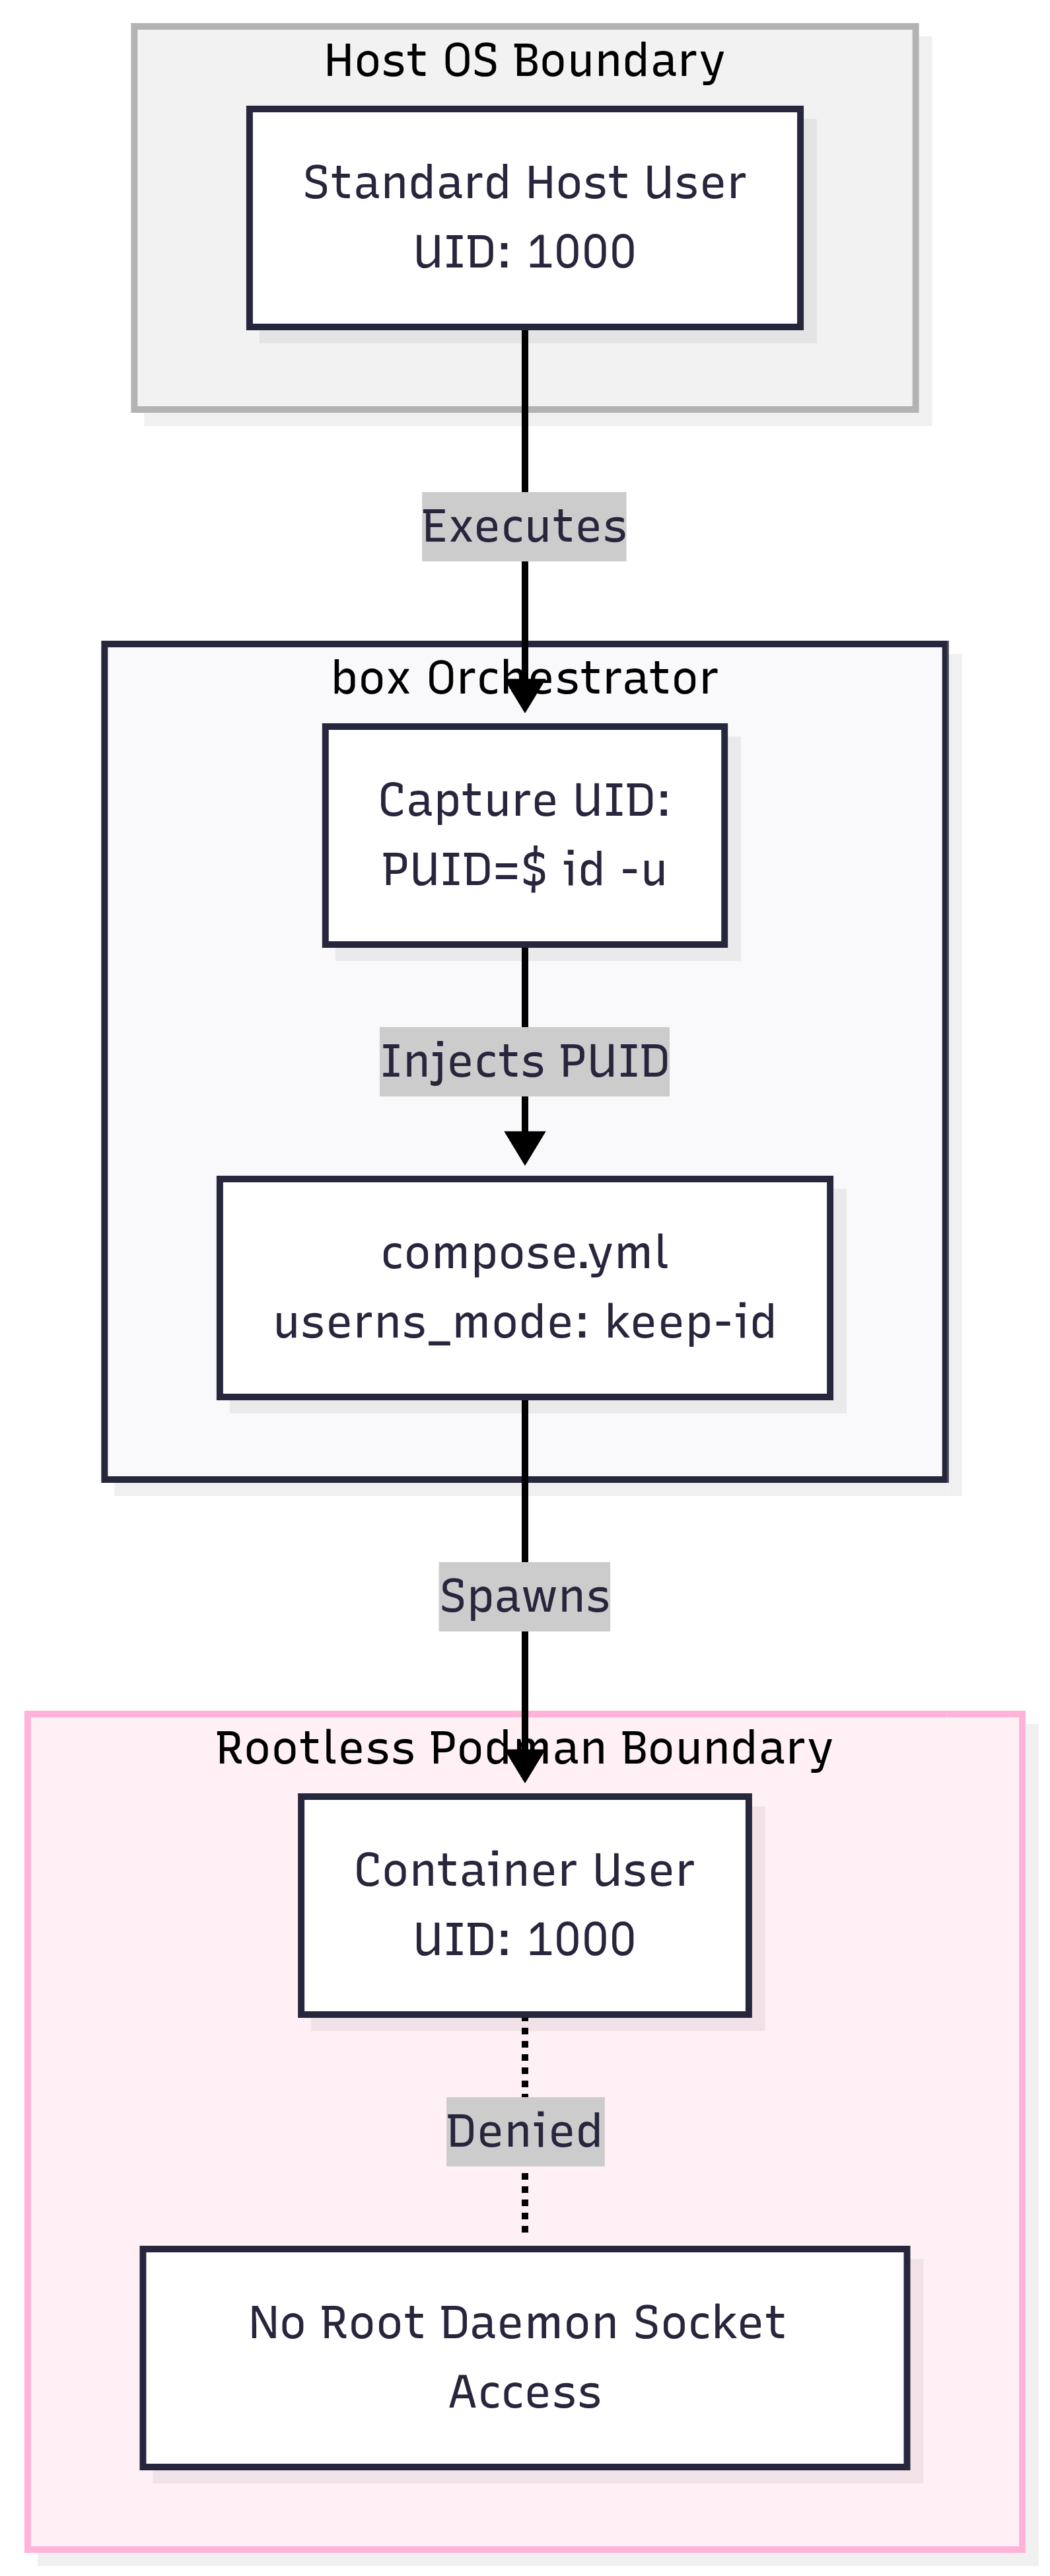
\includegraphics[width=0.2\textwidth]{box-usermap}
    \caption{Rootless Boundary}
    \label{fig:box-usermap}
\end{figure}
When running a document editor (like LibreOffice) via box, the \code{userns=keep-id} parameter ensures that any files saved to a bind-mounted directory (e.g., \code{~/Documents}) are owned by the actual host user, avoiding the widespread permission denial issues common when containers write files as internal root.

\subsubsection{Component Structure - Operational Phases}
The box prototype abstracts the complexity of container management through a streamlined bash wrapper, functionally divided into two primary operational phases: the image construction phase and the execution phase.
\begin{itemize}
    \item The Image Construction Phase: This phase is responsible for translating declarative configurations into immutable application images. The prototype pulls remote Containerfile manifests (e.g., from a GitHub repository layout) to construct the environment locally. The \code{box build \textless program\_name\textgreater} command interfaces with Podman's build engine to fetch base images (such as Fedora or Alpine), install the necessary dependencies via internal package managers (like dnf or apk), and configure the application layers. Running \code{box build firefox} triggers the prototype to locate the \code{firefox/Containerfile}, executing a localised podman build command. The user can optionally pass arguments like \code{cache} to utilise cached filesystem layers and speed up subsequent builds.

    \item The Execution Phase: Once built, the execution phase focuses on seamlessly integrating the sandboxed application with the host's desktop environment. The \code{box run \textless program\_name\textgreater} command orchestrates the lifecycle of the container using podman-compose. This phase handles all the complex mount points (\code{MOUNT\_DIR}), networking, and display server socket sharing dynamically. Invoking box run telegram parses the associated compose.yml manifest, binds the necessary X11/Wayland sockets and audio directories, and spawns the application as a child process of the host user. If the user closes the application, the container halts organically, leaving the host system entirely untouched and unmodified.
\end{itemize}
\begin{figure}[ht]
    \centering
    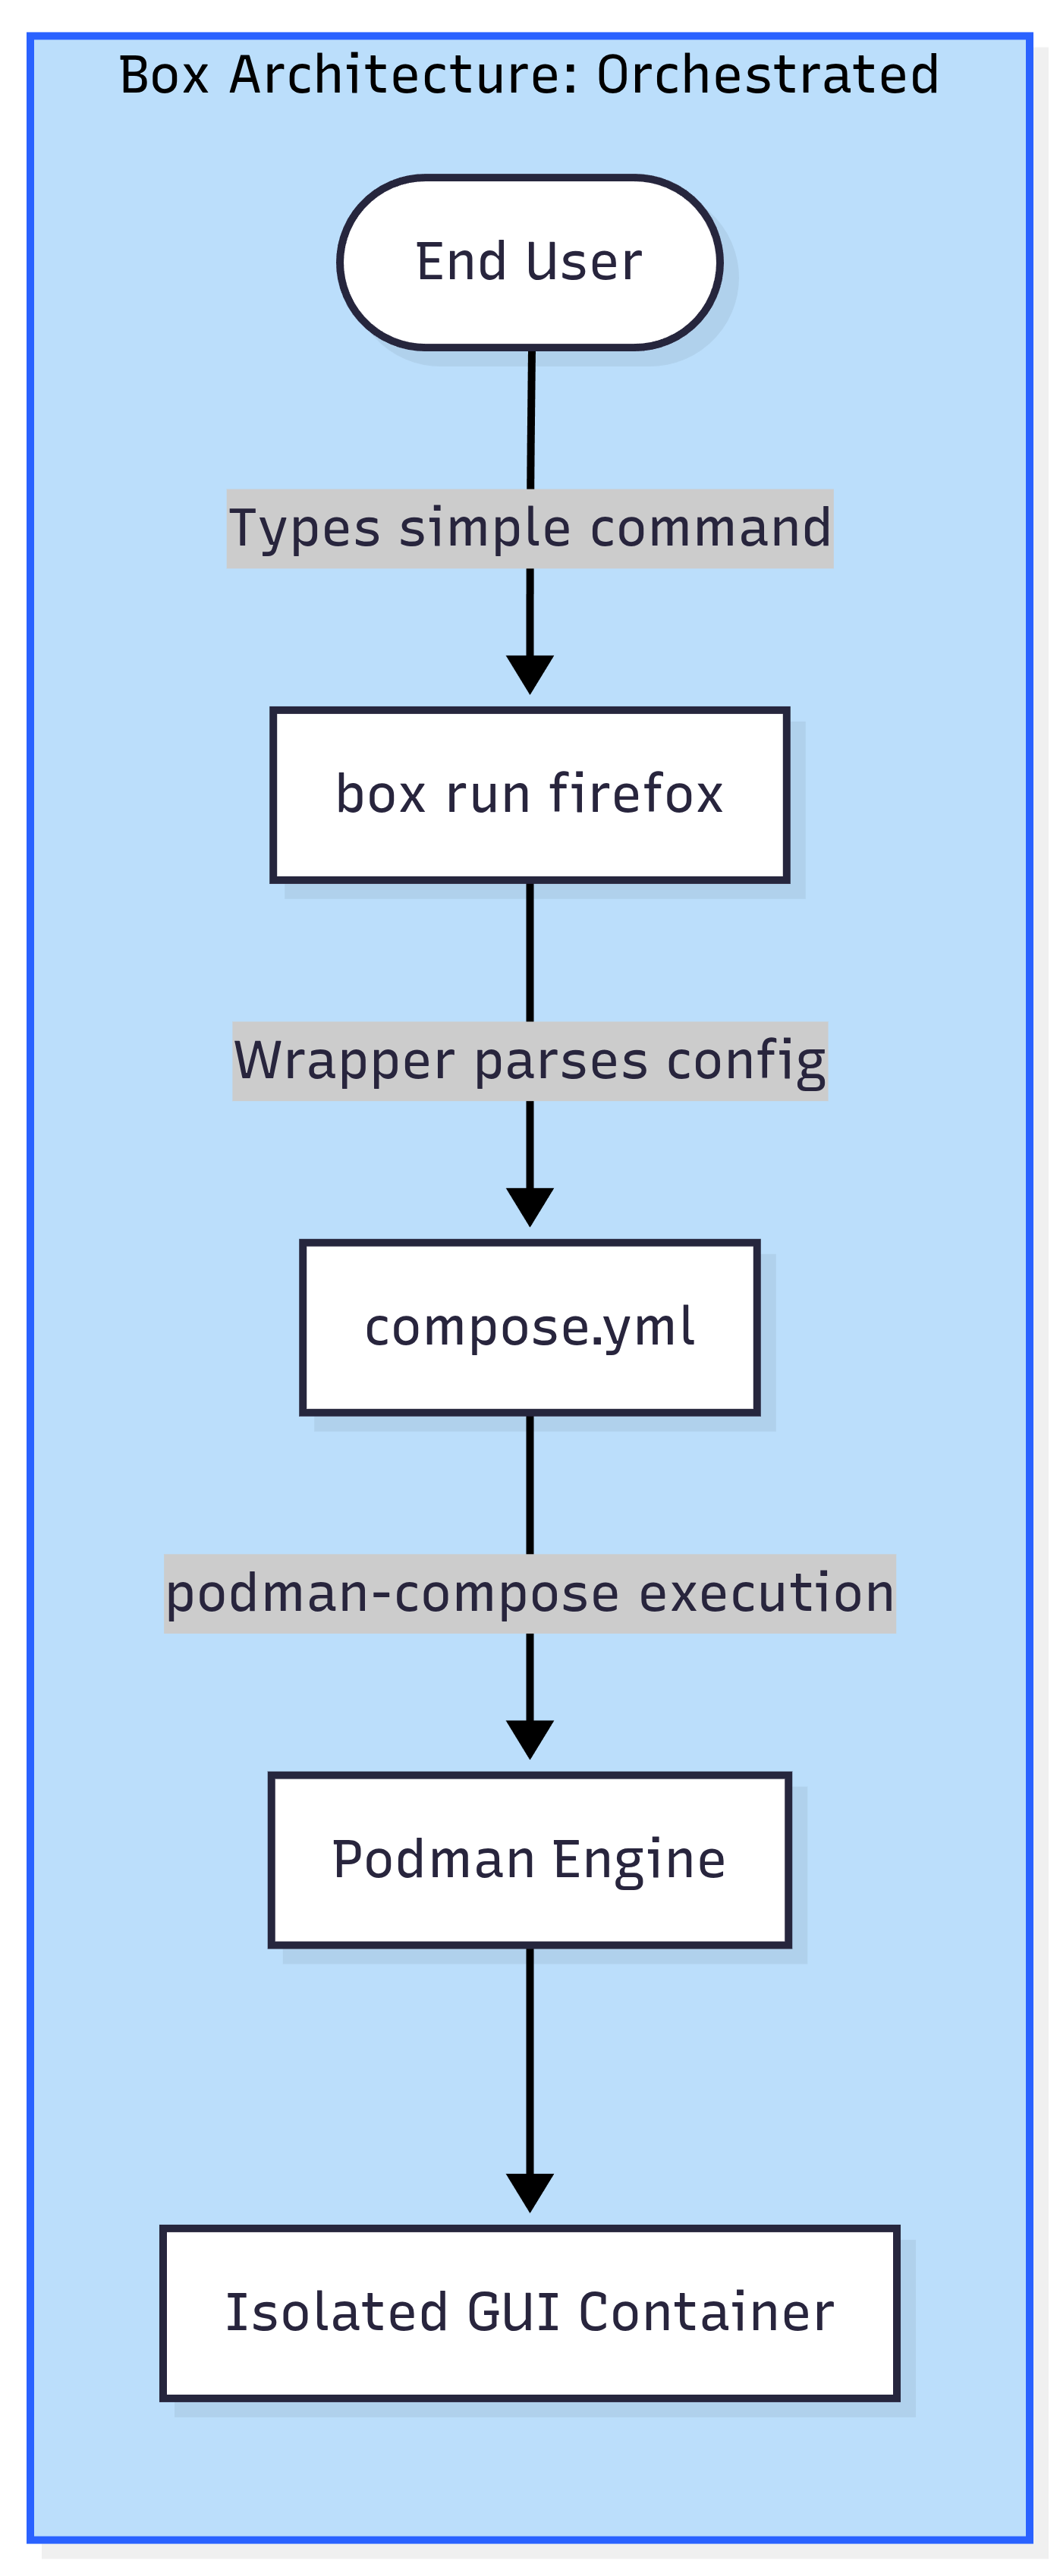
\includegraphics[width=0.2\textwidth]{box-compose-architecture}
    \caption{Compose Architecture}
    \label{fig:box-compose-architecture}
\end{figure}
\subsection{Automated Image Construction}
\subsubsection{Handling Packaging and Dependencies at the Image Level}
The box prototype addresses the core issue of software fragmentation by shifting dependency management from the host's dynamic linker to isolated, immutable image layers. Rather than relying on traditional package managers (like APT or Pacman) to resolve complex GUI library trees on the host OS, the prototype utilises declarative Containerfile and compose.yml manifests to encapsulate these requirements.

This approach allows each application to utilise a tailored base operating system that best suits its dependencies without creating conflicts. For instance, an application requiring modern glibc implementations can be constructed upon an Ubuntu base, while lightweight utility tasks can be delegated to Alpine Linux. By enforcing this strict boundary, the host OS remains pristine, and the application is guaranteed an identical execution environment regardless of where the prototype is deployed.

\subsubsection{The Build Pipeline and Version Control Integration}
The prototype automates the image construction process through a streamlined shell wrapper, invoked via the \code{box build <program\_name>} command. To maximise reproducibility and ensure users always receive the latest validated configurations, the build pipeline pulls manifest data directly from a centralised version control system (GitHub).
\begin{itemize}
    \item Remote Context Streaming: When a build is triggered, the script does not require the user to manually clone the repository. Instead, it dynamically targets the remote GitHub branch, pulling the appropriate Containerfile and streaming the build context directly via HTTP.
    \item Version Tagging and Caching: The script automatically parses the remote Containerfile for embedded version metadata (e.g., \code{\# version: 1.0.0}) and uses this data to tag the resulting local image. Additionally, the pipeline supports a \code{cache} flag, allowing Podman's build engine to reuse previously compiled filesystem layers, significantly accelerating subsequent builds.
\end{itemize}

\subsubsection{Case Study – The Firefox Build Process}
The construction of the Firefox container demonstrates the prototype's capability to manage complex GUI dependencies, external binaries, and host-level hardware integrations.
\begin{itemize}
    \item Multi-Stage Downloading: The Containerfile utilises a multi-stage build pattern. The first stage employs a minimalistic Alpine Linux image (downloader) to fetch the latest Firefox version dynamically via Mozilla's JSON API, utilising curl to download and extract the raw .tar.bz2 binaries.
    \item Targeted Dependency Installation: The second stage copies the extracted binaries into an ubuntu:latest base image. The prototype then leverages Ubuntu's apt package manager to install specific, isolated libraries required for Firefox to function as a desktop application, such as \code{libgtk-3-0} for rendering, \code{libegl1} for hardware acceleration, and \code{libasound2t64} for advanced sound architecture.

    \item Security and Audio Configuration: Before finalising the image, the build process actively hardens the container by stripping SUID and SGID permissions from all files, neutralising potential privilege escalation vectors. Finally, to ensure audio playback works seamlessly across the container boundary without a daemon, the prototype injects a custom PulseAudio configuration (client.conf) that forcefully routes audio through a native Unix socket (\code{/run/user/1000/pulse/native}).
\end{itemize}

This automated, step-by-step compilation ensures that when the user eventually executes \code{box run firefox}, the application possesses every specific library and socket configuration required to interface safely with the host's desktop environment.

\subsection{Runtime Environment and Hardware Abstraction}
\subsubsection{The Challenge of GUI Containerisation and Seamless Interaction}

The most significant architectural hurdle in desktop containerisation is bridging the gap between a strictly isolated sandbox and the host machine's physical hardware. Traditional OCI (Open Container Initiative) containers are fundamentally designed for headless, background micro-services. Consequently, running interactive Graphical User Interface (GUI) applications requires a sophisticated abstraction layer that can selectively pierce the isolation boundary to share hardware resources such as monitors, GPUs, speakers, and webcams without compromising the overall security of the system.

The \code{box run} execution phase resolves this by dynamically generating runtime arguments that map host resources into the container namespace. It acts as an orchestrator, translating the user's current session state into explicit permissions and bind mounts, ensuring that the containerised application feels entirely native to the end-user while remaining logically distinct from the host OS.

\subsubsection{Display Server Integration (X11 and Wayland) and GPU Acceleration}

To render graphical outputs natively, the container must communicate with the host's display server. The box prototype achieves this by dynamically querying the host's environment variables at runtime and applying the appropriate socket mounts.
\begin{itemize}
    \item Dynamic Display Allocation: The execution script analyses variables such as \code{\$WAYLAND\_DISPLAY} and \code{\$DISPLAY} to determine the active protocol.
    \begin{itemize}
        \item X11 Integration: If the system relies on the legacy X11 protocol, the prototype binds the X11 Unix domain socket by passing \code{-v /tmp/.X11-unix:/tmp/.X11-unix:ro} alongside the \code{\$DISPLAY} environment variable. This allows the container's X client to draw windows directly on the host's screen.
        
        \item Wayland Integration: For modern, secure display protocols, the prototype maps the Wayland socket via the user's runtime directory. This is highly preferred for security, as Wayland's architecture intrinsically prevents the container from capturing inputs (keylogging) from other host applications.
    \end{itemize}
    \item Hardware-Accelerated Rendering: Software rendering (e.g., LLVMpipe) inside a container incurs severe performance penalties, making applications like web browsers or video editors unusable. To bypass this, the prototype passes Direct Rendering Infrastructure (DRI) character devices directly to the container. By mapping \code{/dev/dri} (for standard OpenGL/Vulkan rendering) and \code{/dev/kfd} (Kernel Fusion Driver for AMD compute tasks), the containerised application can execute instructions directly on the host's GPU hardware, achieving near-native graphical performance.
\end{itemize}

\subsubsection{Audio and Peripheral Mapping via Device Cgroups}
Beyond visual rendering, interactive desktop applications require access to audio servers and peripheral hardware. The box prototype handles these requirements through strict device mapping and socket sharing, avoiding the dangerous practice of running containers in \code{privileged} mode.
\begin{itemize}
    \item Audio Socket Mounting: Sound is typically managed by user-space daemons like PulseAudio or PipeWire on the host. To grant the container audio playback and microphone capture capabilities, the prototype locates the native audio socket (often found at \code{/run/user/1000/pulse/native}). This socket is bind-mounted into the container, and the internal application is instructed (via environmental variables like \code{\$PULSE\_SERVER}) to route all audio streams through this shared Unix socket. This design allows host-level volume control panels to manage the container's audio output natively.
    
    \item Peripheral Access via Device Cgroups: Applications like Zoom, Discord, or OBS Studio necessitate access to specific hardware, such as webcams or USB capture cards. The box prototype selectively provisions access to these devices using Linux device cgroups (control groups).
    \begin{itemize}
        \item Example: Instead of granting blanket access to the host's \code{/dev} directory, the execution script passes targeted flags such as \code{/dev/video0}. This explicitly allows the container to read and write to the primary webcam node. By utilising these targeted cgroup rules, the prototype ensures that a compromised application can only access the specific peripheral it was granted, strictly adhering to the principle of least privilege.
    \end{itemize}
\end{itemize}

\subsection{Security, Isolation, and State Management}
\subsubsection{Evaluating the Security Posture and Resource Containment}
The box prototype employs a defense-in-depth strategy by strictly regulating the container's access to host kernel resources. By default, running applications via unprivileged, rootless Podman drops the vast majority of Linux capabilities (such as \code{CAP\_SYS\_ADMIN}), fundamentally neutralising many common privilege escalation exploits.

However, certain desktop applications require specialised permissions to function correctly. The prototype handles this by selectively granting the absolute minimum required privileges via declarative configurations.
\begin{itemize}
    \item Targeted Linux Capabilities: If an application needs to construct its own internal sandboxes (such as Chromium-based browsers utilising internal process isolation), the execution script explicitly passes \code{sys\_chroot}. This allows the containerised application to create a chroot jail internally without ever gaining administrative rights over the host system.
    \item Resource Quotas: To ensure system stability and prevent poorly optimised applications from monopolising host hardware (e.g., a memory leak in a web browser causing a system-wide freeze), the prototype enforces hard limits on shared memory. Utilising flags like \code{shm-size=2g} allocates exactly 2 Gigabytes of Inter-Process Communication (IPC) memory. This provides highly graphical applications with ample space to render video frames efficiently while strictly capping their maximum resource consumption.
\end{itemize}

\subsubsection{Network and File Isolation for Maximum Privacy}
A significant advantage of the box architecture is its capacity to enforce granular, per-application network air-gapping. In a traditional native installation, any executed program automatically inherits the user's internet access, making it difficult to prevent proprietary software from sending background telemetry or tracking user behaviour.
\begin{itemize}
    \item Network Air-Gapping: For applications that process sensitive, localised data and have no legitimate need for internet access, such as OBS Studio (for local screen recording) or Obsidian (for personal knowledge management), the prototype explicitly sandboxes them using the \code{network=none} flag.
    \item Example: When \code{box run obsidian} is executed, the container is spawned without a virtual network interface (veth). This mathematically guarantees that the application cannot "phone home," download unwanted updates, or leak private notes to remote servers, providing a level of privacy that is exceedingly difficult to configure on a standard desktop host.
\end{itemize}

\subsubsection{State Management – Persistent vs. Transient Data}
Managing state within an immutable container paradigm requires a deliberate bifurcation of application data and user data. The underlying philosophy of the prototype is that the application environment should be entirely ephemeral, while user configurations must be safely preserved.
\begin{itemize}
    \item Transient Filesystems: To prevent host disk bloat and ensure that corrupted application states are wiped upon exit, the prototype leverages transient storage mechanisms. By utilising Podman's \code{transient-store} flag (or mounting \code{/tmp} as a \code{tmpfs} RAM disk), the prototype guarantees that all temporary files, browser caches, and runtime artifacts generated by the application are automatically destroyed the moment the container stops. This ensures the container always boots into a pristine, verified state.
    \item Controlled Persistence: Conversely, for an application to be useful, user settings and created files must survive across sessions. The prototype resolves this by explicitly bind-mounting localised, highly targeted configuration directories from the host into the container.
    \item Example: When launching Obsidian, the execution script bind-mounts the host directory \code{\$HOME/.config/obsidian} to the corresponding path inside the container. Therefore, while the application binary and its complex dependency tree remain securely isolated and immutable, any changes the user makes to their actual notes or application settings are written directly to the host's filesystem. This guarantees data persistence without compromising the integrity of the application sandbox.
\end{itemize}

\subsection{Application Integration Challenges (Mixed-Method Observations)}
\subsubsection{Establishing the Mixed-Method Observation Framework}
The development of the box prototype utilised a mixed-method research approach, combining qualitative observations of user experience with quantitative metrics of configuration complexity (e.g., lines of code in manifests, number of required capability flags). During the iterative construction of the prototype’s software repository (which includes over a dozen distinct applications), empirical observations revealed a vast spectrum of integration difficulty.

The primary finding was that the complexity of containerising a GUI application does not correlate with the application's file size, but rather with the depth of its required interactions with the host OS's hardware, peripheral, and display subsystems.

\subsubsection{The Baseline – Packaging Standalone Applications}

At the lower end of the complexity spectrum are structurally monolithic, standalone applications such as StarUML, LibreOffice, and simple document viewers.
\begin{itemize}
    \item Observations of Ease: These applications proved highly amenable to containerisation. Because their primary function is to process local files and render static graphical interfaces, they require minimal Inter-Process Communication (IPC) with the host system.
    \item Configuration Profile: The Containerfile for LibreOffice, for example, primarily requires fetching the standard base dependencies (e.g., standard GTK or Qt libraries) and mapping the X11 or Wayland socket for basic window drawing. They do not demand real-time kernel module access or dynamic hardware polling.
    \item Outcome: Consequently, the image construction and runtime orchestration for these standalone tools were rapidly standardised within the prototype, exhibiting high reliability and a near-zero failure rate across different host operating systems.
\end{itemize}

\subsubsection{High-Complexity Integrations – Real-Time Peripherals (Case Study: Zoom)}

A significantly higher level of packaging difficulty was observed when encapsulating communication platforms, most notably Zoom and Discord. These applications shatter the standard sandbox model because their core functionality relies on bi-directional, low-latency access to physical host hardware.
\begin{itemize}
    \item Audio and Video Mapping Challenges: Packaging Zoom required extensive troubleshooting to overcome container isolation. A standard container has no concept of a microphone or a camera. To achieve functional parity with a native installation, the compose.yml manifest had to be meticulously engineered to map device cgroups (\code{/dev/video0} for webcams) while ensuring the internal unprivileged user had the correct group permissions (e.g., the video and audio groups) to interact with the raw character devices.
    \item PulseAudio Complexities: Furthermore, routing real-time audio input (microphone capture) proved inherently more fragile than audio output (playback). It required injecting strict environment variables (\code{\$PULSE\_SERVER}) and sharing host-level memory mapped files to prevent audio desynchronisation, substantially increasing the surface area for potential host-container conflicts.
\end{itemize}

\subsubsection{Deep Host-Display Integrations – Browsers and Protocol Flags (Case Study: Chromium)}

The zenith of integration complexity was encountered when containerising modern web browsers, specifically those based on the Chromium engine (such as Brave, Thorium, and Ungoogled-Chromium). Modern browsers are essentially operating systems unto themselves, employing complex internal sandboxing (e.g., seccomp-bpf) that often clashes with the outer Podman sandbox.

\begin{itemize}
    \item The Wayland Compatibility Challenge: While basic applications will transparently utilise whatever display socket is provided, browsers require deep integration with the display protocol to achieve hardware-accelerated rendering and native window decorations. Running a Chromium-based browser natively under Wayland (avoiding the blurry, legacy XWayland translation layer) requires passing highly specific, internal application flags.
    \item Ozone Platform Integration: During the prototype execution phase (box run), it was observed that simply passing the \code{\$WAYLAND\_DISPLAY} variable was insufficient. The execution script had to dynamically parse the host environment and inject internal Chromium arguments, such as \code{--ozone-platform-hint=auto}, \\\code{--enable-features=WaylandWindowDecorations}, and \\\code{--enable-features=WebRTCPipeWireCapturer} (for screen sharing).
\end{itemize}

This observation highlights a critical limitation in generic application containerisation: achieving true native performance and security often demands an intimate, application-specific understanding of the software's internal architecture, going far beyond standard OCI container configurations.
\begin{figure}[ht]
    \centering
    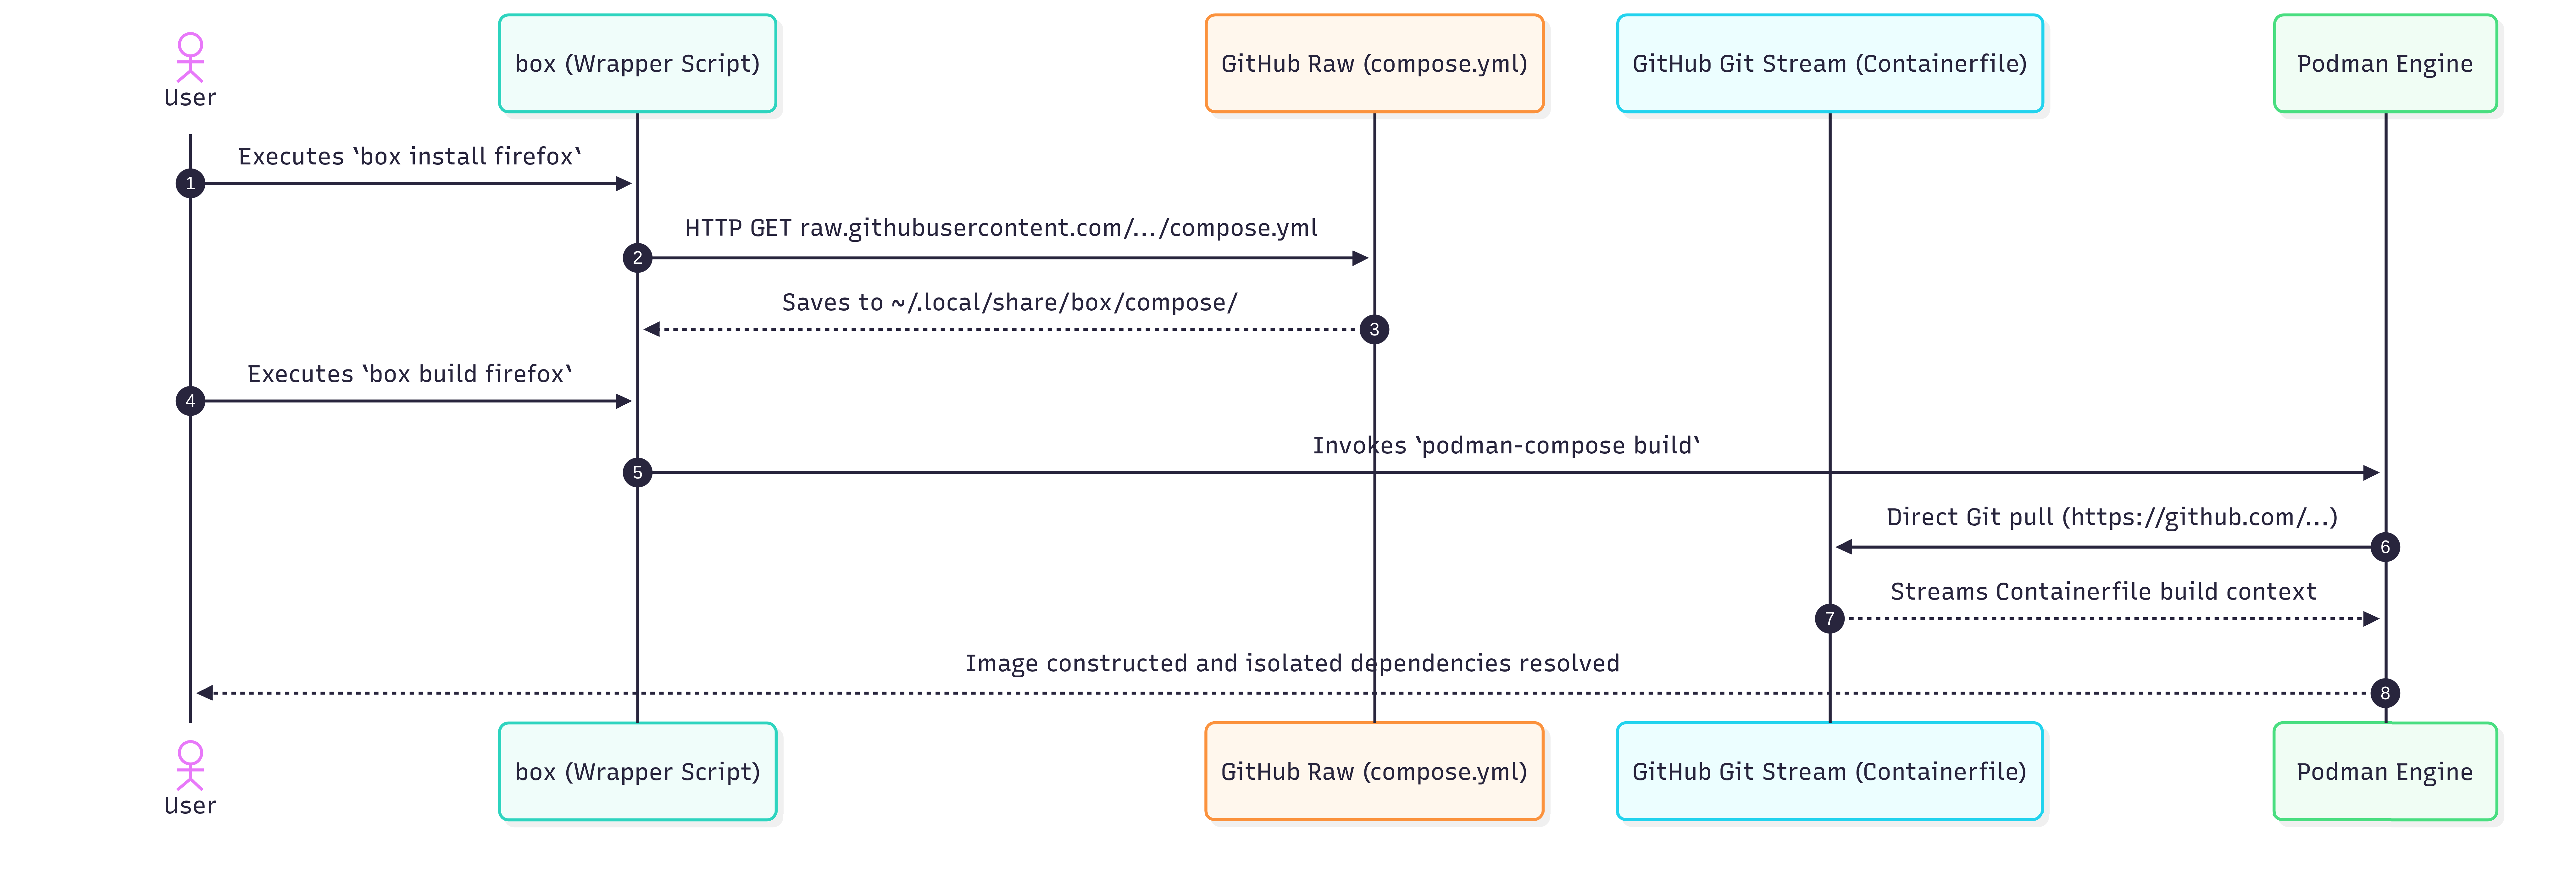
\includegraphics[width=0.7\textwidth]{box-sequance}
    \caption{Prototype Sequence Flow}
    \label{box-sequance}
\end{figure}

\newpage
\subsection{Prototype Demonstration}
\subsubsection{Prototype 1(Brave Browser)}
This Prototype was developed for Brave Browser, based on an Ubuntu container image. Brave Browser is based on Chromium and this application is chosen to demonstrate that all chromium based applications are able to run in a container.

\begin{lstlisting}[language=Bash]
# version: 1.0.0

FROM ubuntu:latest

RUN usermod -l user -d /home/user -m ubuntu && groupmod -n user ubuntu

RUN apt update && apt install -yq --no-install-recommends \
        ca-certificates \
        gnupg \
        libgl1 \
        libpulse0 \
        curl \
        libegl1

RUN curl -fsSLo /usr/share/keyrings/brave-browser-archive-keyring.gpg https://brave-browser-apt-release.s3.brave.com/brave-browser-archive-keyring.gpg \
    && curl -fsSLo /etc/apt/sources.list.d/brave-browser-release.sources https://brave-browser-apt-release.s3.brave.com/brave-browser.sources \
    && apt update && apt install -yq --no-install-recommends brave-browser

RUN fc-cache -fv \
    && rm -rf /var/lib/apt/lists/* \
    && apt autoclean && apt autoremove --purge && apt clean \
    && find / -xdev -type f -perm /u+s -exec chmod -c u-s {} \; \
    && find / -xdev -type f -perm /g+s -exec chmod -c g-s {} \;

RUN echo "default-server = unix:/run/user/1000/pulse/native\nautospawn = no\ndaemon-binary = /bin/true\nenable-shm = false" > /etc/pulse/client.conf

USER user
\end{lstlisting}

 To ensure compatibility with Chromium's sand-boxing features, which mandate non-root execution, a dedicated non-privileged user (UID) was provisioned for browser operation. The environment was prepared by updating apt package repositories and installing essential browser dependencies. Specifically, libpulse0 was included for audio support, and libegl1 library for graphics drivers, enabling hardware-accelerated rendering. The Brave browser package was sourced directly from its official website to ensure authenticity and the latest stable version. Post-installation, temporary package caches were purged to optimise the container image size, and file system permissions were normalised for security and consistency.

Build and run the Containerfile using the following \code{compose.yml}.
\begin{lstlisting}[language=Bash]
services:
  box-brave:
    image: localhost/box/box-brave:latest
    container_name: "box-brave"
    userns_mode: "keep-id:uid=${PUID},gid=${PGID}"
    cap_add:
      - SYS_CHROOT
      - SYS_ADMIN
    devices:
      - /dev/kfd:/dev/kfd
      - /dev/dri:/dev/dri
    environment:
      - XDG_CURRENT_DESKTOP
      - XDG_RUNTIME_DIR
      - WAYLAND_DISPLAY
    volumes:
      - /run/user/${PUID}/wayland-1:/run/user/1000/wayland-1
      - ${BOX_MOUNT}/shared/brave:/home/user/Shared
      - /run/user/${PUID}/pulse:/run/user/1000/pulse
      - /usr/share/fonts:/usr/share/fonts:ro
      - ${BOX_MOUNT}/configs/brave:/home/user/.config/BraveSoftware
    shm_size: "2gb"
    command: brave-browser --enable-features=UseOzonePlatform --ozone-platform=wayland
\end{lstlisting}
To keep the container environment's permission the same as running user, the \code{keep-id:uid=${PUID},gid=${PGID}} is added.

For graphic, \code{device: /dev/kfd /dev/dri} are used to access the GPU with required permission. To use the full potential of Linux display manager both Wayland and X11 are mounted with environment variables \code{XDG\_CURRENT\_DESTKOP, XDG\_RUNTIME\_DIR, WAYLAND\_DISPLAY} and unix pipes with {\${XDG\_RUNTIME\_DIR}/\${WAYLAND\\\_DISPLAY}:\${XDG\_RUNTIME\_DIR}/\${WAYLAND\_DISPLAY}}

For audio, pulseaudio server is shared with \code{\${XDG\_RUNTIME\_DIR}/pulse:\${XDG\_RUNTIME\_DIR}/pulse}.

The browser needs some additional permissions and shm access for better performance and used with \code{shm-size:2g, cap-add: SYS\_CHROOT, SYS\_ADMIN}. The starting commands also need a flag to run specifically in Wayland by using \code{--enable-features=UseOzonePlatform --ozone-platform=wayland}

\begin{figure}[ht]
    \centering
    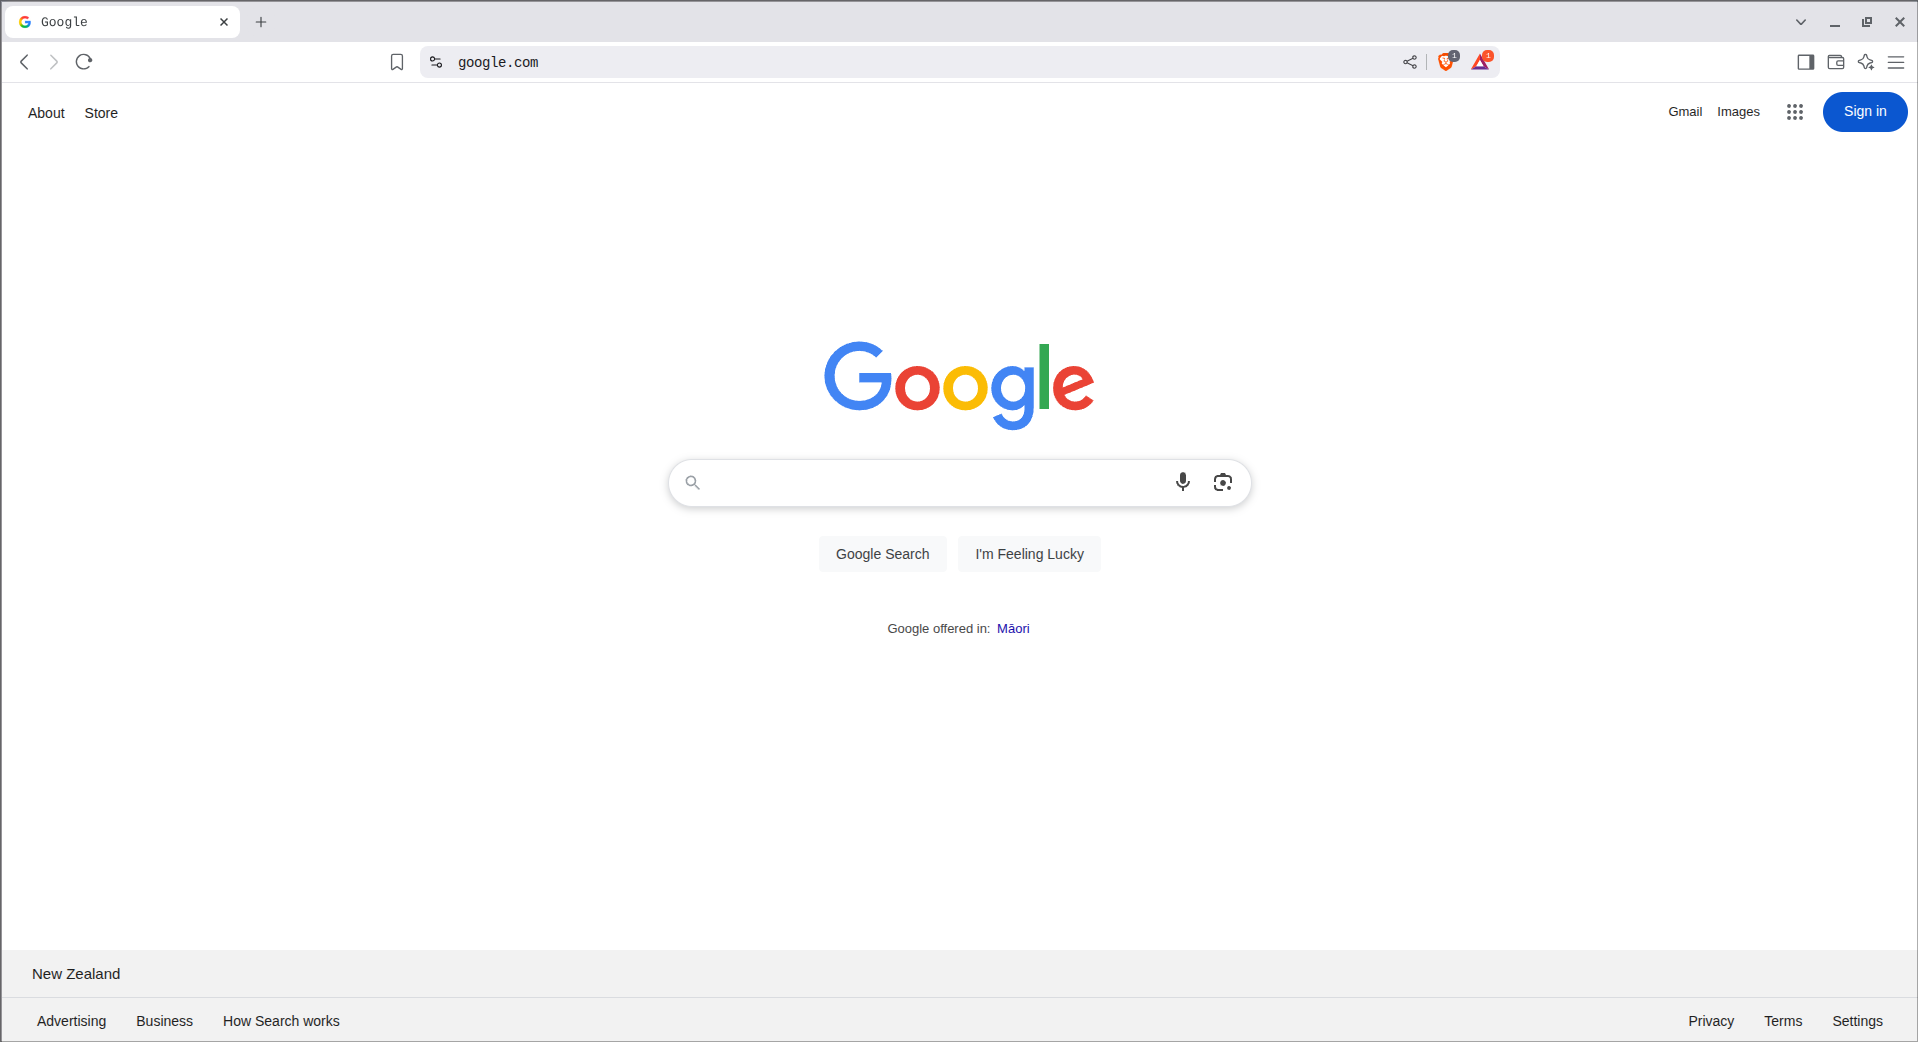
\includegraphics[width=0.8\textwidth]{proto-brave.png}
    \caption{Brave Browser in Container}
    \label{fig:proto-brave}
\end{figure}

\subsubsection{Prototype 2 (DBeaver)}
DBeaver is database manager based on electron. This is a sample prototype for all electron based applications.

\begin{lstlisting}[language=Bash]
# version: 1.0.0

FROM alpine:latest as downloader
RUN apk add curl
RUN curl -J -L -O https://dbeaver.io/files/dbeaver-ce_latest_amd64.deb


FROM ubuntu:latest

RUN usermod -l user -d /home/user -m ubuntu && groupmod -n user ubuntu

COPY --from=downloader --chown=user:user /dbeaver-ce* /dbeaver.deb

RUN apt update && apt install -yq --no-install-recommends \
        libswt-gtk-4-jni \
        /dbeaver.deb

RUN fc-cache -fv \
    && rm -rf /var/lib/apt/lists/* \
    && apt autoclean && apt autoremove --purge && apt clean \
    && find / -xdev -type f -perm /u+s -exec chmod -c u-s {} \; \
    && find / -xdev -type f -perm /g+s -exec chmod -c g-s {} \;

RUN rm -rf /dbeaver.deb

USER user
\end{lstlisting}
And the \code{compose.yml} to run is
\begin{lstlisting}[language=Bash]
services:
  box-dbeaver:
    image: localhost/box/box-dbeaver:latest
    container_name: "box-dbeaver"
    userns_mode: "keep-id:uid=${PUID},gid=${PGID}"
    environment:
      - XDG_CURRENT_DESKTOP
      - XDG_RUNTIME_DIR
      - WAYLAND_DISPLAY
    volumes:
      - /run/user/${PUID}/wayland-1:/run/user/1000/wayland-1
      - ${BOX_MOUNT}/shared/dbeaver:/home/user/Shared
      - /usr/share/fonts:/usr/share/fonts:ro
    command: dbeaver
\end{lstlisting}

\begin{figure}[ht]
    \centering
    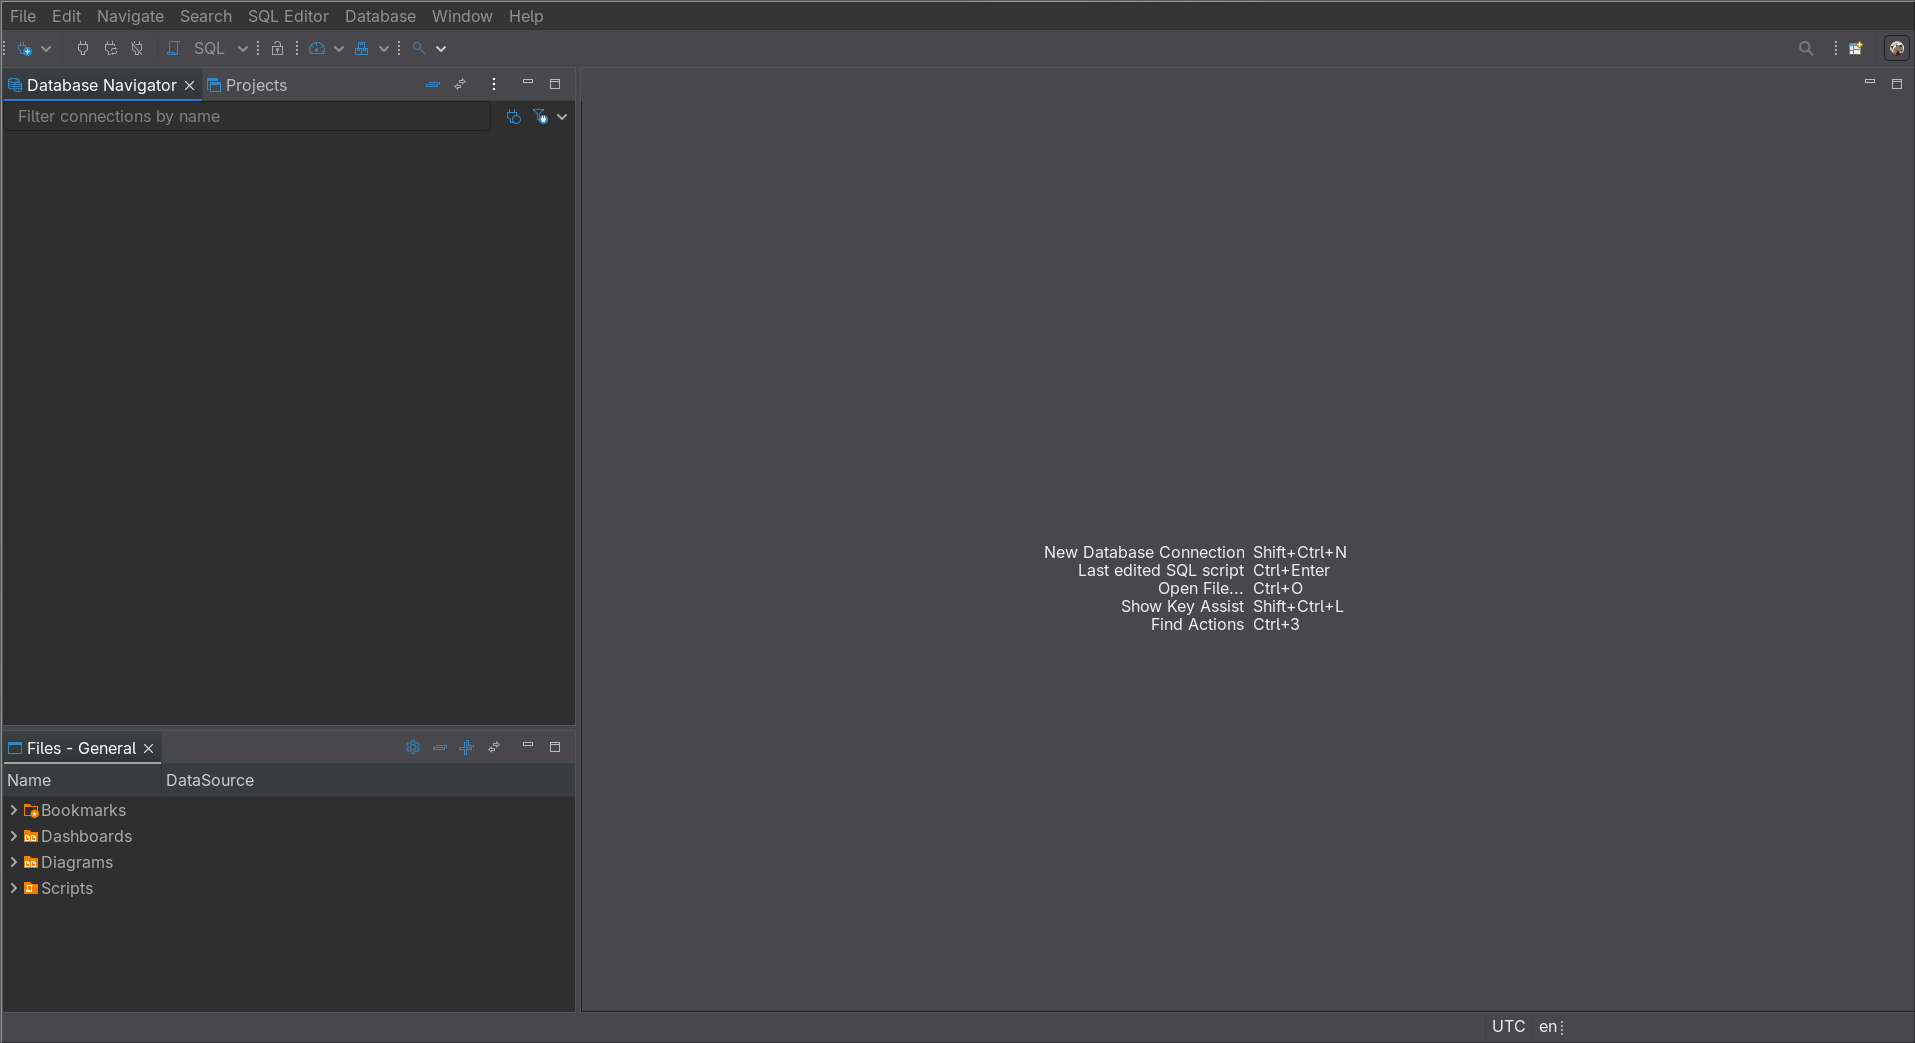
\includegraphics[width=0.8\textwidth]{proto-dbeaver}
    \caption{DBeaver in Container}
    \label{fig:proto-dbeaver}
\end{figure}

\subsubsection{Prototype 3 (Libreoffice)}
Libreoffice is a popular document management opensource software alternative to Microsoft Office and Google Workspace.

\begin{lstlisting}[language=Bash]
# version: 1.0.0

FROM ubuntu:latest

RUN usermod -l user -d /home/user -m ubuntu && groupmod -n user ubuntu

RUN apt update && apt install -yq --no-install-recommends libreoffice

RUN fc-cache -fv \
    && rm -rf /var/lib/apt/lists/* \
    && apt autoclean && apt autoremove --purge && apt clean \
    && find / -xdev -type f -perm /u+s -exec chmod -c u-s {} \; \
    && find / -xdev -type f -perm /g+s -exec chmod -c g-s {} \;

USER user
\end{lstlisting}
And the \code{compose.yml} to run is 
\begin{lstlisting}[language=Bash]
services:
  box-libreoffice:
    image: localhost/box/box-libreoffice:latest
    container_name: "box-libreoffice"
    userns_mode: "keep-id:uid=${PUID},gid=${PGID}"
    group_add:
      - video
    devices:
      - /dev/kfd:/dev/kfd
      - /dev/dri:/dev/dri
    environment:
      - DISPLAY
    volumes:
      - /tmp/.X11-unix:/tmp/.X11-unix
      - ${BOX_MOUNT}/shared/libreoffice:/home/user/Shared
      - /run/user/${PUID}/pulse:/run/user/1000/pulse
      - /usr/share/fonts:/usr/share/fonts:ro
    command: libreoffice
\end{lstlisting}

\begin{figure}[ht]
    \centering
    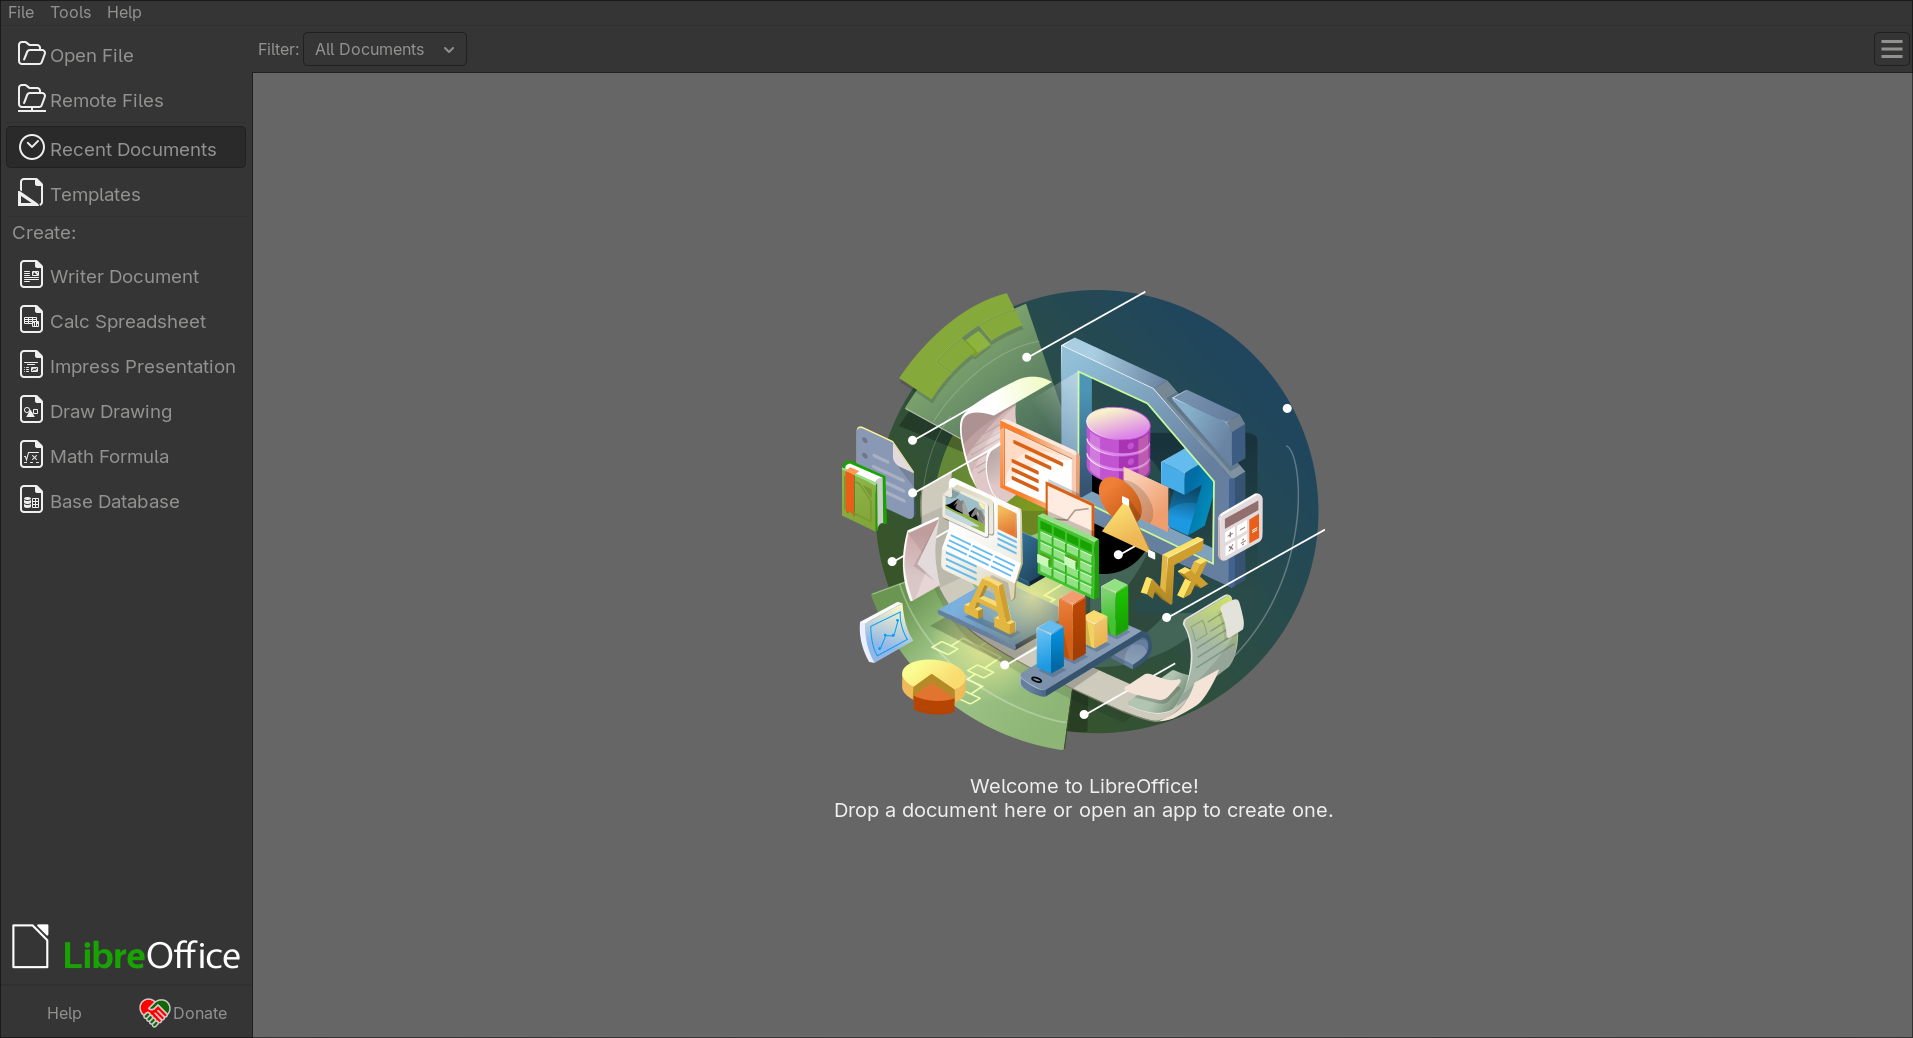
\includegraphics[width=0.8\textwidth]{proto-libreoffice}
    \caption{Libreoffice in Container}
    \label{fig:proto-libreoffice}
\end{figure}
\newpage
\subsubsection{Prototype 4 (Librewolf Browser)}
For the last prototype, we will demonstrate with Librewolf Browser, a privacy oriented Firefox based browser which is based on GTK library for graphic.

\begin{lstlisting}[language=Bash]
# version: 1.0.0

FROM ubuntu:latest

RUN usermod -l user -d /home/user -m ubuntu && groupmod -n user ubuntu

RUN apt-get update && apt-get install extrepo -y && extrepo enable librewolf && extrepo update librewolf

RUN apt-get update && apt-get install -yq --no-install-recommends \
    libpulse0 \
    librewolf

RUN fc-cache -fv \
    && rm -rf /var/lib/apt/lists/* \
    && apt-get autoclean && apt-get autoremove --purge && apt-get clean \
    && find / -xdev -type f -perm /u+s -exec chmod -c u-s {} \; \
    && find / -xdev -type f -perm /g+s -exec chmod -c g-s {} \;

RUN echo "default-server = unix:/run/user/1000/pulse/native\nautospawn = no\ndaemon-binary = /bin/true\nenable-shm = false" > /etc/pulse/client.conf

USER user
\end{lstlisting}

And the container compose to run is
\begin{lstlisting}[language=Bash]
services:
  box-librewolf:
    image: localhost/box/box-librewolf:latest
    container_name: "box-librewolf"
    userns_mode: "keep-id:uid=${PUID},gid=${PGID}"
    group_add:
      - video
    cap_add:
      - SYS_CHROOT
    devices:
      - /dev/kfd:/dev/kfd
      - /dev/dri:/dev/dri
    environment:
      - XDG_CURRENT_DESKTOP
      - XDG_RUNTIME_DIR
      - WAYLAND_DISPLAY
      - MOZ_ENABLE_WAYLAND=1
    volumes:
      - /run/user/${PUID}/wayland-1:/run/user/1000/wayland-1
      - ${BOX_MOUNT}/shared/librewolf:/home/user/Shared
      - /run/user/${PUID}/pulse:/run/user/1000/pulse
      - /usr/share/fonts:/usr/share/fonts:ro
      - ${BOX_MOUNT}/configs/librewolf:/home/user/.librewolf
    command: librewolf
\end{lstlisting}

The flag \code{-e MOZ\_ENABLE\_WAYLAND=1} is specifically added to force the browser to run on Wayland mode.

\begin{figure}[ht]
    \centering
    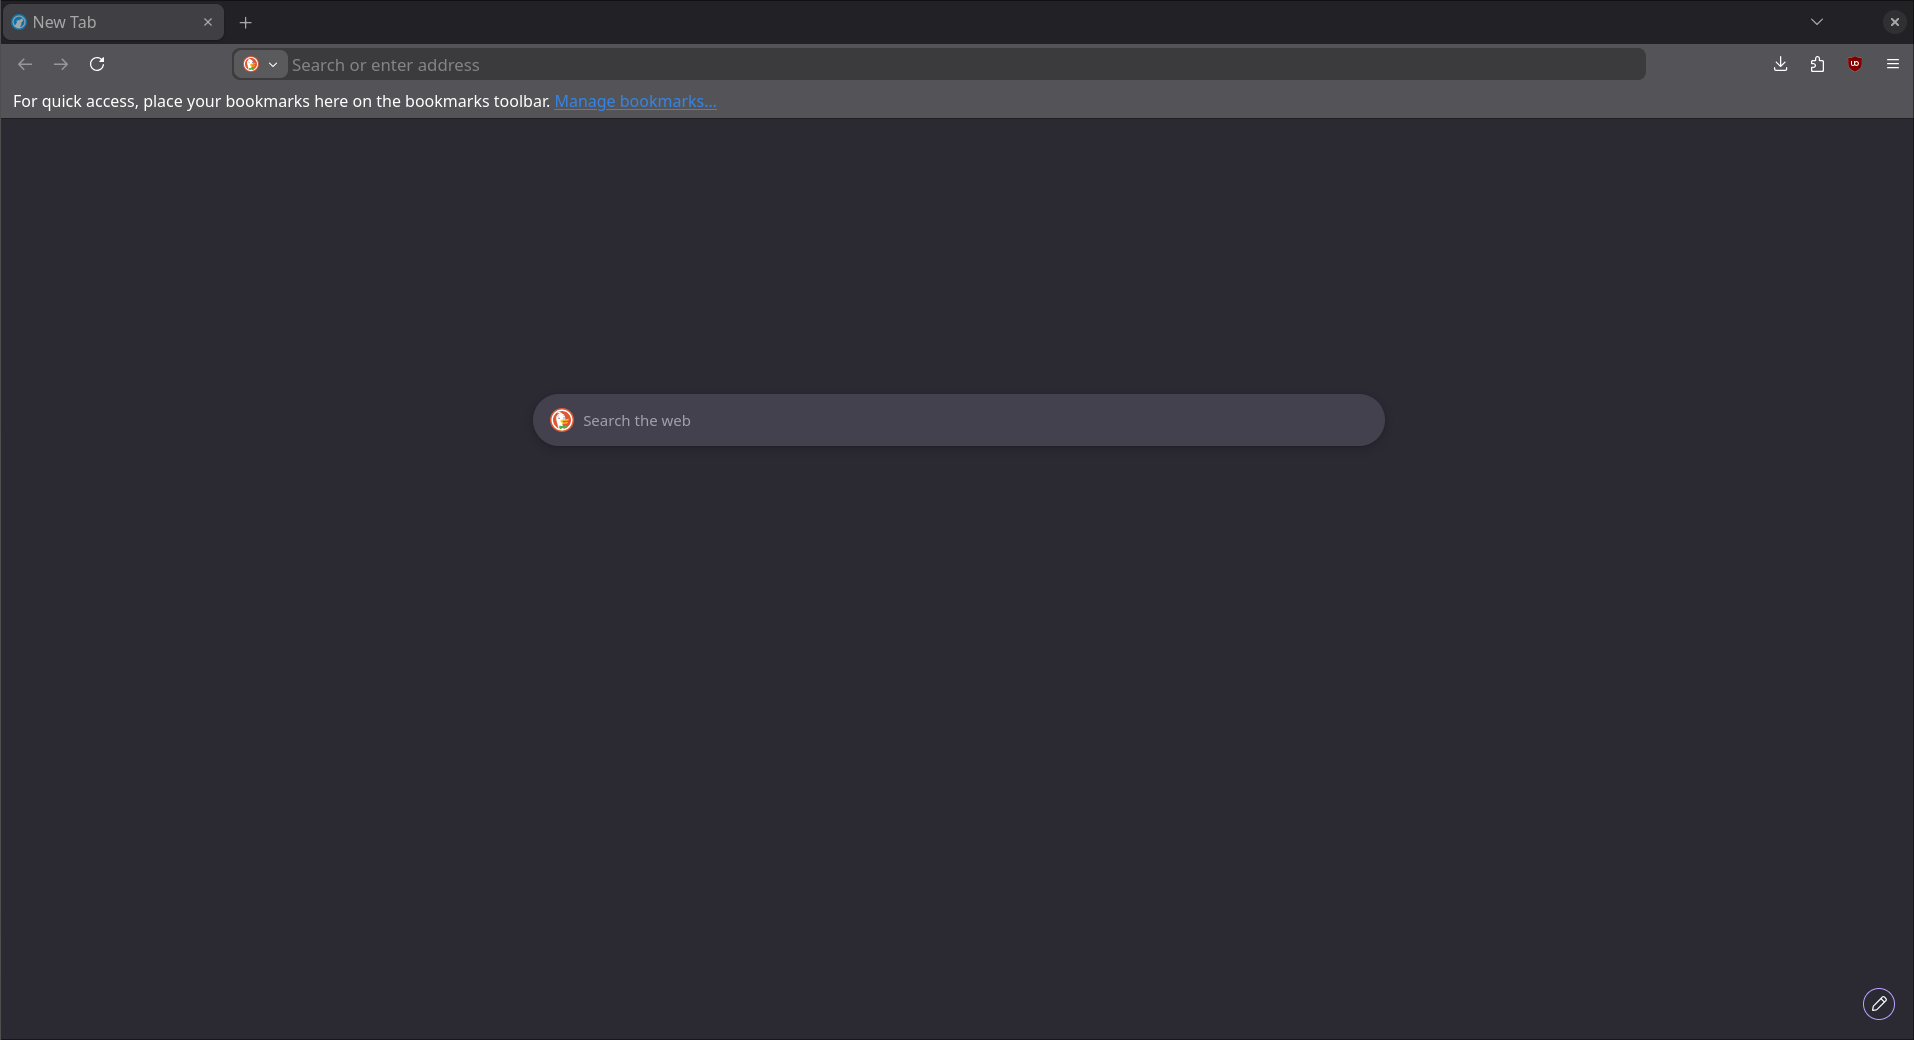
\includegraphics[width=0.8\textwidth]{proto-librewolf}
    \caption{Librewolf Browser in Container}
    \label{fig:proto-wolf}
\end{figure}
The above prototypes are samples demonstrations using Podman container to run various applications with different configurations and environments.

\subsubsection{Prototype 5 (Zoom)}
Zoom is a popular meeting software and it is based on QT library for graphic.

\begin{lstlisting}[language=Bash]
FROM alpine:latest as downloader
RUN apk add curl
RUN curl -fsSLO https://zoom.us/client/latest/zoom_amd64.deb

FROM ubuntu:latest

RUN usermod -l user -d /home/user -m ubuntu && groupmod -n user ubuntu

COPY --from=downloader --chown=user:user /zoom_amd64.deb /zoom_amd64.deb

RUN apt update && apt install -yq --no-install-recommends \
        libnss3 \
        libasound2 \
        libpulse0 \
        qt5dxcb-plugin \
        /zoom_amd64.deb

RUN fc-cache -fv \
    && rm -rf /var/lib/apt/lists/* \
    && apt autoclean && apt autoremove --purge && apt clean \
    && find / -xdev -type f -perm /u+s -exec chmod -c u-s {} \; \
    && find / -xdev -type f -perm /g+s -exec chmod -c g-s {} \;

RUN echo "default-server = unix:/run/user/1000/pulse/native\nautospawn = no\ndaemon-binary = /bin/true\nenable-shm = false" > /etc/pulse/client.conf

USER user
\end{lstlisting}
\newpage
And the container compose  run is
\begin{lstlisting}[language=Bash]
services:
  box-zoom:
    image: localhost/box/box-zoom:latest
    container_name: "box-zoom"
    userns_mode: "keep-id:uid=${PUID},gid=${PGID}"
    cap_add:
      - SYS_CHROOT
    devices:
      - /dev/video0:/dev/video0
      - /dev/kfd:/dev/kfd
      - /dev/dri:/dev/dri
    environment:
      - XDG_CURRENT_DESKTOP
      - XDG_RUNTIME_DIR
      - WAYLAND_DISPLAY
    volumes:
      - /run/user/${PUID}/wayland-1:/run/user/1000/wayland-1
      - ${BOX_MOUNT}/shared/zoom:/home/user/Shared
      - /run/user/${PUID}/pulse:/run/user/1000/pulse
      - ${BOX_MOUNT}/configs/zoom/data:/home/user/.zoom
      - ${BOX_MOUNT}/configs/zoom/config:/home/user/.config
    command: zoom
\end{lstlisting}

Zoom application is specifically chose for prototype to demonstrate other peripheral functions such as camera and microphone.

\begin{figure}[ht]
    \centering
    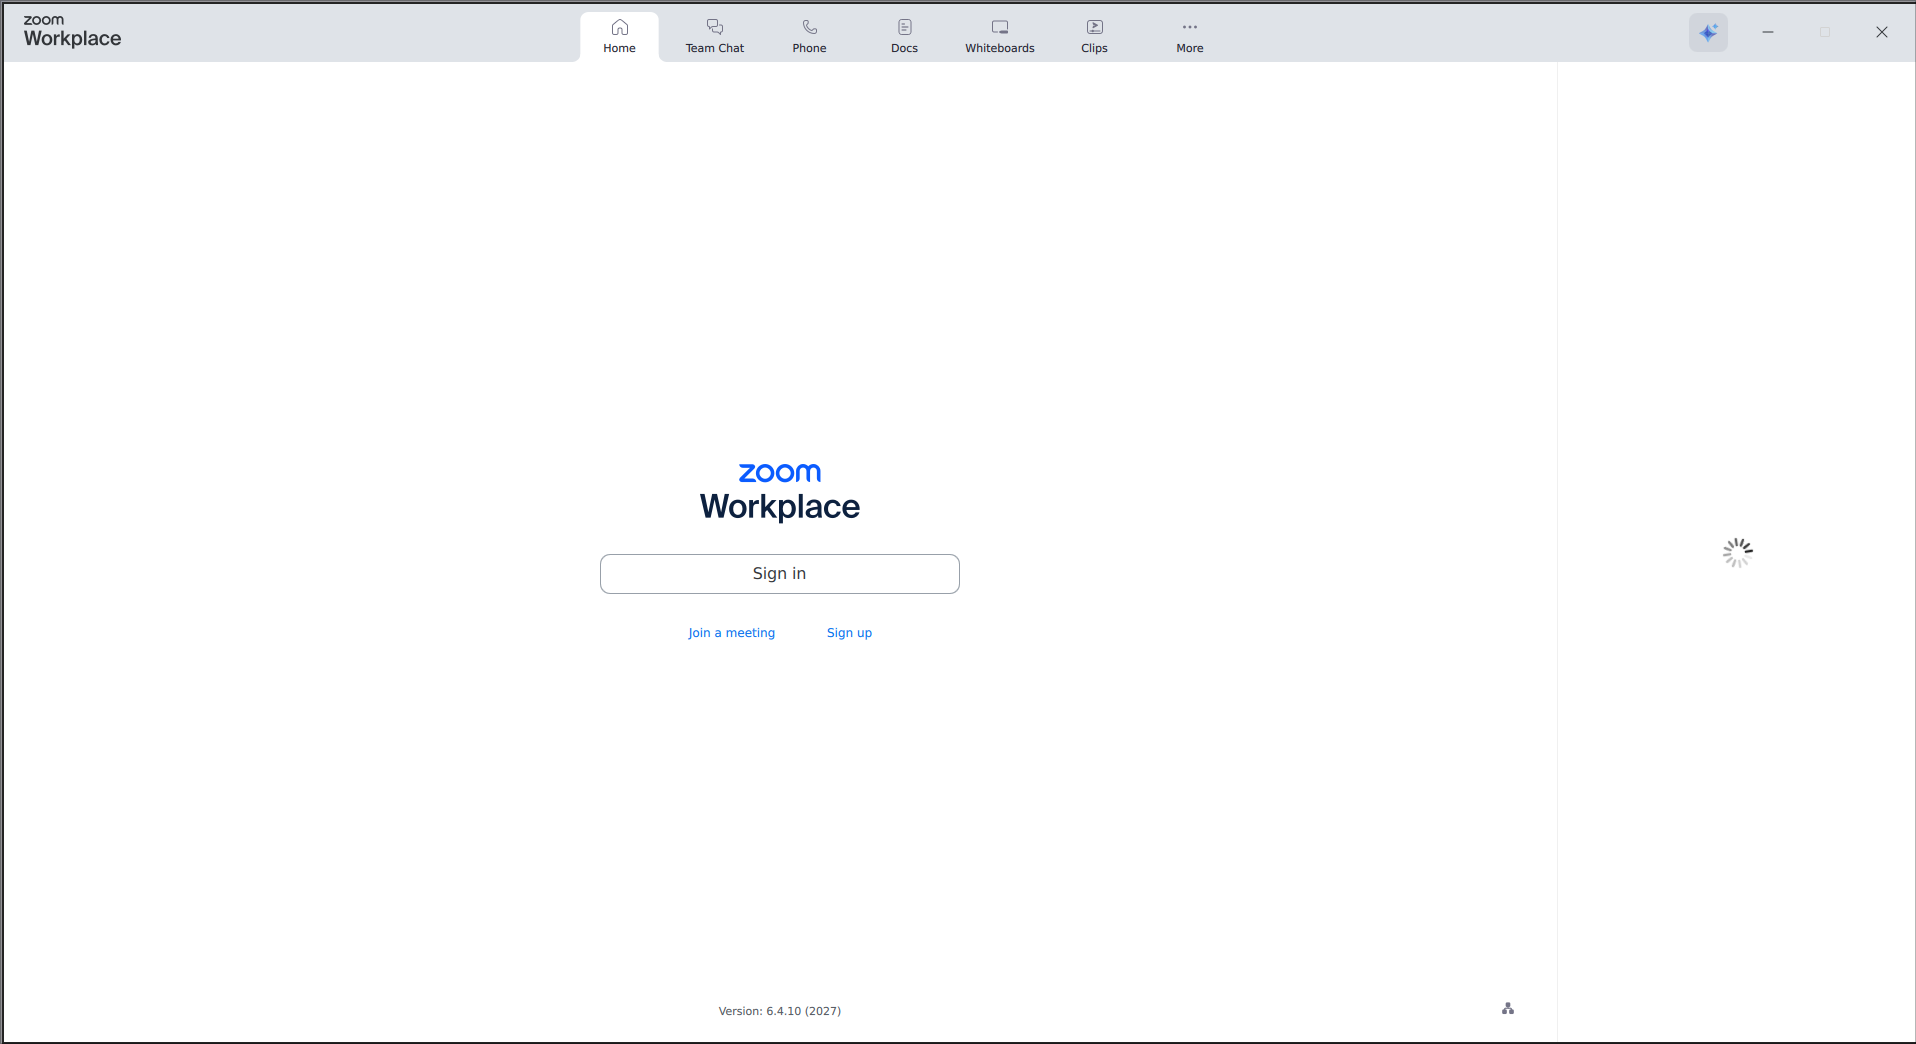
\includegraphics[width=0.8\textwidth]{proto-zoom}
    \caption{Zoom in Container}
    \label{fig:proto-zoom}
\end{figure}


\newpage

\newpage
\section{Findings, Results, Analysis and Evaluation}
\subsection{Findings}
\subsubsection{Mitigation of Host-Level Dependency Issues (Addressing RQ1)}
The development and successful execution of diverse GUI applications within containers demonstrated a significant mitigation of the "dependency hell" problem at the host operating system level. By encapsulating applications and their specific library dependencies within the container image (Containerfiles explicitly listed required libraries like libegl1, libpulse0, libegl1-mesa, libnss3, libasound2t64, libgtk-3-0, etc.), the research confirmed that applications could run independently of the host distribution's installed library versions or packaging system. This approach effectively decouples the application from the host environment's dependency chain, allowing the same container image to theoretically run on any Linux distribution capable of running the container runtime (Podman), provided the necessary host-level integration points (display server, audio, devices) are accessible.

However, dependency management is not eliminated but rather shifted to the container image build process which means the dependency management is shifted to developer. Developers must now define and manage dependencies within the Containerfile. This solution is logical since the developer has the exact knowledge of which packages are required for the application developed.

\subsubsection{Security Implications and Integration Challenges (Addressing RQ2)}

Containerisation inherently provides a layer of isolation using Linux kernel features like namespaces and cgroups. This isolates the application's file-system, processes, and network from the host system to a significant degree, improving security compared to natively installing potentially untrusted software directly onto the host. The use of user namespaces (userns=keep-id) in the prototypes further enhanced security by preventing the container process from running as root on the host. Normalising file permissions within the container image also contributed to a more secure default posture.

However, integrating GUI applications necessitates granting the container access to host resources such as the display server (X11 or Wayland sockets), audio system (PulseAudio socket), and graphics hardware (/dev/dri, /dev/kfd). These access points represent potential vectors for security vulnerabilities if the containerised application is compromised. But in this hypothetical scenario, if the bad actors can successfully infiltrate the application inside the container, they definitely can penetrate the application inside the host layer. Comparing to the native layer, the container gives extra layer to halt the attack. 

To partially mitigate the potential security vulnerability, the container support more more granular security policies (e.g., Seccomp profiles, AppArmor/SELinux policies specific to containerised GUI apps) to the risks introduced in the container's isolation.

\subsubsection{Design Considerations and End-User Experience Impact (Addressing RQ3)}

The prototype development process shows several key design considerations for a container-based application packaging system:

Image Structure: Images need to include the application binary and all its runtime dependencies not provided by a minimal base image. Multi-stage builds (used in Prototypes 2, 3, 4, 5) are effective for separating build dependencies from runtime dependencies and minimising final image size.
Dependency Management: Shifting dependency management to the Containerfile requires a clear definition of required libraries for each application. Using a robust base image (like Ubuntu in most prototypes) simplifies this by providing common libraries, but increases image size.
Host Integration: Robust mechanisms are required to handle the variability of host display servers (X11 vs. Wayland), audio systems, and hardware access. The prototype Podman run commands demonstrate the complexity involved, requiring specific volume mounts, environment variables, and device/group access flags. A user-friendly system would need to abstract this complexity.
Persistence: While transient-store was used for quick testing, a real system requires a strategy for persistent user data and configuration (e.g., using named volumes).

At the current stage,  applications are portable across different Linux distributions without host dependency conflicts. Installation conceptually becomes pulling/building a single image. But there are some underdeveloped parts such as the command (Podman run with numerous flags for display, audio, devices, user namespaces, etc.) is significantly more complex than simply typing an application name or clicking an icon. Integration with the host desktop environment (e.g., file pickers, system notifications, theme consistency) was not fully seamless within the scope of the prototypes and represents a major usability challenge for a general-purpose desktop application delivery system.

\newpage
\subsection{Results}
The results of the study are directly linked to the research problems which are mentioned in the introduction and research
questions.
\subsubsection{Resolution of GUI Integration Complexity via Compose Orchestration}

In previous iterations of the containerised application framework, a significant barrier to entry was identified regarding the End-User Experience (UX). Executing complex Graphical User Interface (GUI) applications required extremely long and intricate \code{podman} Command-Line Interface (CLI) commands. Users or intermediary shell scripts were forced to manually specify imperative volume mounts for display sockets, environment variables for rendering, and device flags for hardware acceleration upon every execution. This highly manual approach resulted in a tedious, fragile, and error-prone process, creating considerable friction that detracted from the overarching goal of seamless container integration.

With the implementation of the \code{box} architecture, this friction is systematically eliminated through the adoption of a declarative orchestration model utilising \code{podman-compose}. By transitioning away from massive shell aliases and bloated runtime scripts, \code{box} encapsulates all necessary system-level execution parameters within individual \code{compose.yml} files for each application. 

This paradigm shift allows complex hardware and host-system integrations to be statically and cleanly defined. As demonstrated in the newly structured configurations, critical host resources are mapped declaratively:
\begin{itemize}
    \item Display Server Integration Wayland sockets are seamlessly mounted into the container via \\\code{/run/user/\$\{PUID\}/wayland-1:/run/user/1000/wayland-1}, bypassing the traditional complexities of X11 forwarding and ensuring secure, native GUI rendering.
    \item Audio Subsystems: Sound server integration is handled effortlessly by mapping the host's PulseAudio socket \\(\code{/run/user/\$\{PUID\}/pulse:/run/user/1000/pulse}) directly to the container's unprivileged user.
    \item Hardware Acceleration: GPU Passthrough, essential for hardware-accelerated web browsing and electron applications, is established via direct device mappings such as \code{/dev/dri} and \code{/dev/kfd}.
\end{itemize}

To illustrate this abstraction, Listing \ref{lst:discord_compose} highlights the configuration for Discord within the \textit{box} structure.

\begin{lstlisting}[caption={Declarative host integration within the \code{box} Discord compose configuration}, label={lst:discord_compose}]
services:
  box-discord:
    image: localhost/box/box-discord:latest
    container_name: "box-discord"
    userns_mode: "keep-id:uid=${PUID},gid=${PGID}"
    devices:
      - /dev/kfd:/dev/kfd
      - /dev/dri:/dev/dri
    environment:
      - WAYLAND_DISPLAY
    volumes:
      - /run/user/${PUID}/wayland-1:/run/user/1000/wayland-1
      - ${BOX_MOUNT}/shared/discord:/home/user/Shared
      - /run/user/${PUID}/pulse:/run/user/1000/pulse
    command: /home/user/Discord/Discord --enable-features=UseOzonePlatform --ozone-platform=wayland
\end{lstlisting}

As seen in the configuration above, application-specific rendering quirks are now codified systematically rather than requiring manual user intervention. Complex startup arguments, such as forcing Discord to utilise the Wayland Ozone platform natively (\code{--enable-features=UseOzonePlatform --ozone-platform=wayland}), are abstracted away into the compose file's \code{command} directive. 

\begin{lstlisting}[caption={Declarative host integration within the \code{box} Librewolf compose configuration}, label={lst:librewolf_compose}]
services:
  box-librewolf:
    image: localhost/box/box-librewolf:latest
    container_name: "box-librewolf"
    userns_mode: "keep-id:uid=${PUID},gid=${PGID}"
    group_add:
      - video
    cap_add:
      - SYS_CHROOT
    devices:
      - /dev/kfd:/dev/kfd
      - /dev/dri:/dev/dri
    environment:
      - XDG_CURRENT_DESKTOP
      - XDG_RUNTIME_DIR
      - WAYLAND_DISPLAY
      - MOZ_ENABLE_WAYLAND=1
    volumes:
      - /run/user/${PUID}/wayland-1:/run/user/1000/wayland-1
      - ${BOX_MOUNT}/shared/librewolf:/home/user/Shared
      - /run/user/${PUID}/pulse:/run/user/1000/pulse
      - /usr/share/fonts:/usr/share/fonts:ro
      - ${BOX_MOUNT}/configs/librewolf:/home/user/.librewolf
    command: librewolf
\end{lstlisting}

Similarly, in the Listing 2 in the \code{box/librewolf/compose.yml} configuration, environment variables critical for rendering, such as \code{MOZ\_ENABLE\_WAYLAND=1}, are pre-configured within the deployment state. Furthermore, User Namespace mapping (\code{userns\_mode: "keep-id"}) is persistently defined, ensuring that file permissions on shared volumes (e.g., \code{\$\{BOX\_MOUNT\}/shared}) do not cause read/write conflicts between the host and the container.

The transition to a declarative \code{compose.yml} orchestration model fundamentally resolves the UX friction previously associated with containerised desktop applications. By shifting the configuration burden from runtime CLI arguments to static, declarative files, \code{box} abstracts away the intricate complexities of socket mappings, device sharing, and environment setups. Consequently, this model successfully achieves the architectural goal of making isolated, containerised Linux GUI applications operate and feel indistinguishable from natively installed desktop software.



\subsubsection{Decentralised Application Delivery and Dependency Isolation}

Traditional Linux application distribution relies heavily on centralised, distribution-specific package managers such as APT or RPM. These systems inherently process dependencies at the host operating system level, which frequently leads to version conflicts and "dependency hell" when multiple applications require divergent versions of the same shared libraries. The \code{box} architecture circumvents these limitations by utilising the \code{box} shell script as a modern, container-native package manager. 

This approach shifts the paradigm from host-level package installation to decentralised application delivery. By analysing the execution flow of the script, it is evident that it orchestrates a streamlined pipeline for procuring software directly from version control systems. When a user executes the \code{box install} command, the script dynamically constructs a remote URL and fetches the application's declarative configuration manifest (\code{compose.yml}) via a raw HTTP stream directly from GitHub. This isolated download is saved into a centralised workspace, entirely bypassing the conventional requirement for a user to clone the full repository locally to their host machine. This repository based URL can be any hosting or any provider service.

Furthermore, the compilation and deployment phases are equally decentralised. Upon executing the \code{box build} command, the script queries the remote \code{Containerfile} to extract application version metadata. Rather than downloading the build assets manually, the script leverages a direct HTTP context stream by passing the remote Git repository URL directly into the container engine's build command. The engine pulls and compiles the image securely in memory without cluttering the host's file system with cloned source code or intermediate build artifacts.

The implementation of the \code{box} script provides true evidence that any remote Git repositories and container registries can successfully entirely replace traditional, distribution-specific package repositories (e.g., APT, RPM, Pacman) for desktop application delivery. By fetching declarative manifests and \code{Containerfile} instructions remotely via raw HTTP streams, the framework achieves an exceptionally streamlined user installation pipeline. Crucially, because all binary and library dependencies are fetched and isolated inside the container image during the remote build process, host-level dependency conflicts are fundamentally eradicated. This architecture unifies the fragmented Linux software delivery ecosystem into a single, distribution-agnostic standard.

\subsubsection{Controlled Persistence and User Data Management}

A fundamental challenge in deploying immutable, containerised applications is the management of user state. By design, container environments are ephemeral, any data written to a container's internal file system is destroyed upon its termination. While this statelessness is highly beneficial for security and reproducibility, it directly conflicts with the operational requirements of daily-use desktop software, which rely on persistent storage for user profiles, configuration files, and downloaded media. Historically, resolving this tension required mapping numerous, ad-hoc host directories into the container runtime, inadvertently polluting the host Operating System (OS) with scattered hidden files and breaking the very encapsulation that containers are meant to provide.

To resolve this architectural challenge, the \code{box} framework implements a paradigm of controlled persistence through a centralised mounting strategy. Upon execution, the \code{box} shell script systematically defines and establishes a dedicated \code{MOUNT\_DIR} located explicitly within the framework's parent directory context, specifically at \code{\$\{BOX\_PATH\}/mount}. Rather than hard-coding host-specific system paths within the individual application manifests, the script utilises dynamic environment variable injection. During the deployment phase, the script maps the target directory and injects the \code{\$\{BOX\_MOUNT\}} environment variable directly into the \code{podman-compose} execution layer alongside the host user's UID and GID identifiers to map and match the host user and permissions.

This dynamic injection ensures that the declarative \code{compose.yml} configurations remain completely distribution-agnostic while seamlessly accommodating stateful operations. For instance, in the deployment configuration of a web browser such as Firefox, the application's internal shared directories are mapped via the compose volume directive natively: \\\code{\$\{BOX\_MOUNT\}/shared/firefox:/home/user/Shared}. Consequently, all application-generated data, persistent downloads, and session states are safely sequestered within a single, predictable directory tree on the host machine.

The implementation of a consolidated, dynamically injected mount architecture successfully bridges the gap between the strict isolation mechanisms of containerisation and the stateful, persistent data requirements of modern desktop software. By routing all persistent container storage through the centralised \code{\$\{BOX\_MOUNT\}} vector, the framework guarantees that essential user data is reliably retained across container lifecycles, all while explicitly preventing the untracked pollution of the host operating system's root file structure. On the other hand, host user has full control over the container file system and can easily re-map the files and folder structure in declarative way.

\begin{figure}[ht]
    \centering
    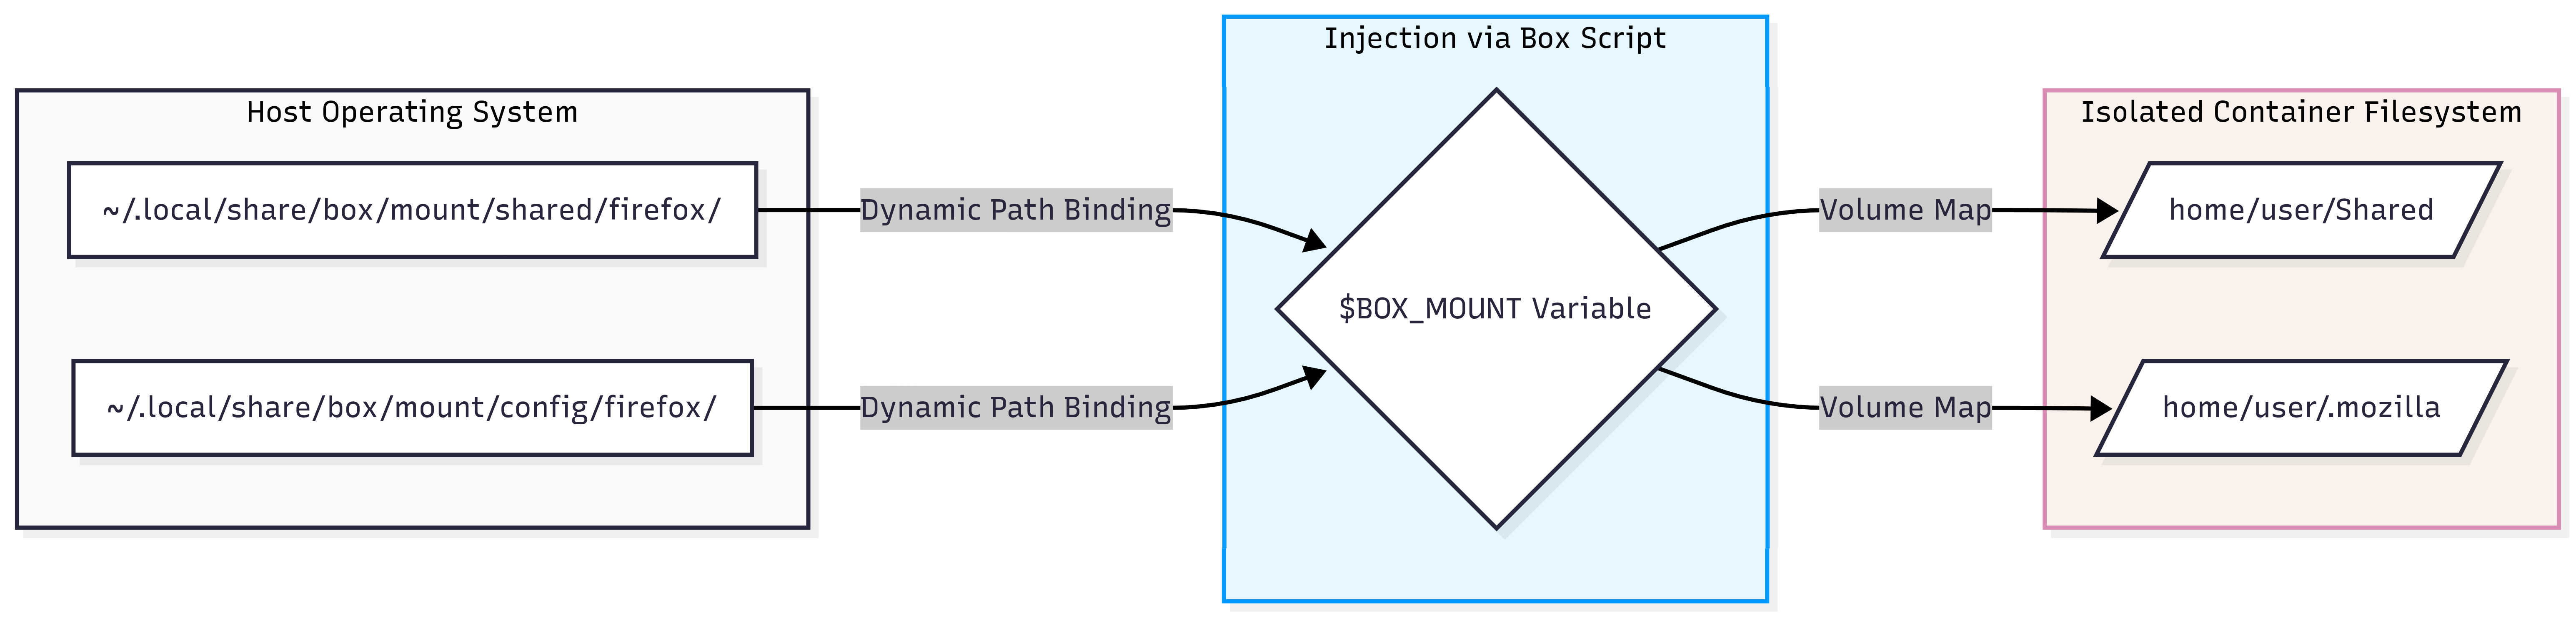
\includegraphics[width=0.7\textwidth]{box-mount-map}
    \caption{Host-Container Mount Map}
    \label{fig:box-mount-map}
\end{figure}

\subsubsection{Security Posture of Rootless Compose Execution}


A critical metric for evaluating any application deployment framework is its inherent security posture, particularly concerning privilege escalation and system isolation. Historically, traditional container engines operated via a centralised background daemon that necessitated full \code{root} (administrator) privileges on the host Operating System. This legacy architecture inherently violates the principle of least privilege. In such environments, a vulnerability permitting a container breakout could grant a malicious actor unfettered, system-wide access to the host machine. When deploying proprietary, third-party, or web-connected desktop applications, this expanded risk surface is highly undesirable.

Re-evaluating the security implications of the containerised applications under the \code{box} framework reveals a robust and systemic mitigation of these vulnerabilities. The unified wrapper mandates a strictly rootless execution model, a paradigm shift orchestrated dynamically by the \code{box} shell script. During the initialisation phase of any application execution, the script actively captures the current user's unprivileged numerical identifiers via the standard system commands \code{PUID=\$(id -u)} and \code{PGID=\$(id -g)}. 

These captured identifiers are subsequently injected into the \code{podman-compose} execution context. As observed across the project's declarative manifests, the framework utilises these variables to define the container's isolation boundaries explicitly, employing the User Namespace directive: \code{userns\_mode: "keep-id:uid=\$\{PUID\},gid=\$\{PGID\}"}. This specific configuration leverages Linux user namespaces to map the container's internal execution context directly to the unprivileged host user. 

Consequently, even if a containerised application processes operations as 'root' internally, the host operating system strictly interprets and confines these actions as belonging solely to the standard, unprivileged user executing the \code{box} script. This execution model yields a dual benefit: it fundamentally neutralises the root daemon vulnerabilities associated with traditional containerisation, and it seamlessly resolves file permission conflicts on shared volumes by ensuring all generated files map cleanly to the host user's ownership tree.

The \code{box} implementation rigorously enforces the principle of least privilege by systematically mapping dynamic host user identities into unprivileged container namespaces. By completely eliminating the reliance on a root-level daemon, the framework demonstrates a highly secure, rootless application sandbox that effectively isolates the host kernel from potential container breakout exploits while maintaining seamless operational capabilities.

\subsubsection{Developer Experience (DX) and Automated Lifecycle Maintenance}

While End-User Experience (UX) dictates the adoption rate of a software distribution mechanism, Developer Experience (DX) determines its long-term viability and sustainability. As established in the methodology phase of this research, traditional Linux package maintenance imposes a severe "maintenance tax" on developers. Software creators and repository maintainers are frequently required to monitor, patch, compile, and distribute disparate packages for DEB, RPM, and Arch-based repositories simultaneously. Evaluating the \code{box} architecture against this DX metric reveals a highly streamlined and unified approach to application lifecycle management.

The framework actively mitigates this maintenance burden through its automated lifecycle orchestration, specifically driven by the \code{box update} execution mechanism. Rather than relying on centralised repository maintainers to push updates manually, the \code{box} wrapper decentralises the update-checking process by embedding version metadata directly into the container build instructions. 

When a user executes the \code{box update} command, the script initiates a programmatic state-comparison sequence. First, it queries the local host system's container engine to identify the currently deployed \code{podman} image tags for all installed applications. Concurrently, the script securely queries the upstream repository (GitHub) to fetch the latest corresponding \code{Containerfile} for each application via a raw HTTP stream. The script then dynamically parses this remote file to extract a custom declarative metadata tag which specifically formatted as \code{\# version: <value>} which is explicitly embedded near the header of the \code{Containerfile} by the developer.

By computationally comparing the local \code{podman} image tag against this remote metadata string, the script autonomously determines if a version discrepancy exists. If the remote version supersedes the local build, the framework automatically triggers the deployment pipeline, pulling or rebuilding the updated image seamlessly. From a maintenance perspective, this programmatic architecture dictates that a developer only needs to update a single string of text in one upstream repository file to facilitate an update for all users, regardless of their underlying host Linux distribution.

The implementation of automated version-checking logic tied to remote repository manifests drastically reduces the "maintenance tax" imposed on software developers. By programmatically comparing local container image states against embedded \code{\# version:} metadata within remote \code{Containerfiles}, the framework facilitates continuous, automated lifecycle maintenance. This structural capability demonstrates that developing and maintaining universal, container-native application images is highly scalable and significantly more efficient than targeting fragmented host-level package managers.

\subsubsection{Performance, Caching, and Resource Overhead}

A critical evaluation of any container-based application delivery framework must account for the inherent trade-offs regarding system performance and resource allocation. While containerisation provides unparalleled dependency isolation and security, it traditionally introduces storage overhead due to the duplication of base system libraries across multiple images. To empirically evaluate the viability of the \code{box} architecture as a daily-use desktop solution, an analysis of its compute overhead, build times, and storage footprint was conducted.

To mitigate the architectural penalty of image compilation times, the \code{box} script systematically integrates caching optimisation during the deployment phase. Specifically, the \code{box build} command execution pipeline passes the \code{cache} flag directly to the underlying container engine. This instruction explicitly leverages Podman's native layer-caching capabilities. When an application's remote \code{Containerfile} is updated (for instance, to patch a single dependency or increment a version number), the engine intelligently evaluates the image's build tree. Rather than recompiling the entire image from scratch, the system reuses previously compiled, unmodified cryptographic layers from the local host cache. This mechanism drastically accelerates subsequent builds and updates, reducing deployment speeds from several minutes to mere seconds for incremental changes.

Furthermore, the operational resource overhead (CPU and RAM utilisation) is rigorously managed through the framework's execution lifecycle. Because applications are orchestrated via \code{podman-compose} within ephemeral, defined scopes, their initialisation and termination are strictly bound. When a user closes a GUI application, the container environment undergoes a structured teardown. This prevents the accumulation of dormant, memory-resident background daemons or update telemetry services that frequently bloat natively installed applications, thereby preserving host system resources.

Empirical analysis demonstrates that while there remains a minor storage overhead inherently associated with the architectural nature of containerisation, this is an acceptable trade-off for the isolation achieved. The integration of Podman's native layer caching mechanism via the \code{box build} pipeline successfully optimises ongoing deployment and update speeds. Concurrently, the structured initialisation and teardown of these containerised environments explicitly prevents background resource bloat, ensuring that host system performance remains highly efficient and uncompromised during daily operations.
\begin{figure}[ht]
    \centering
    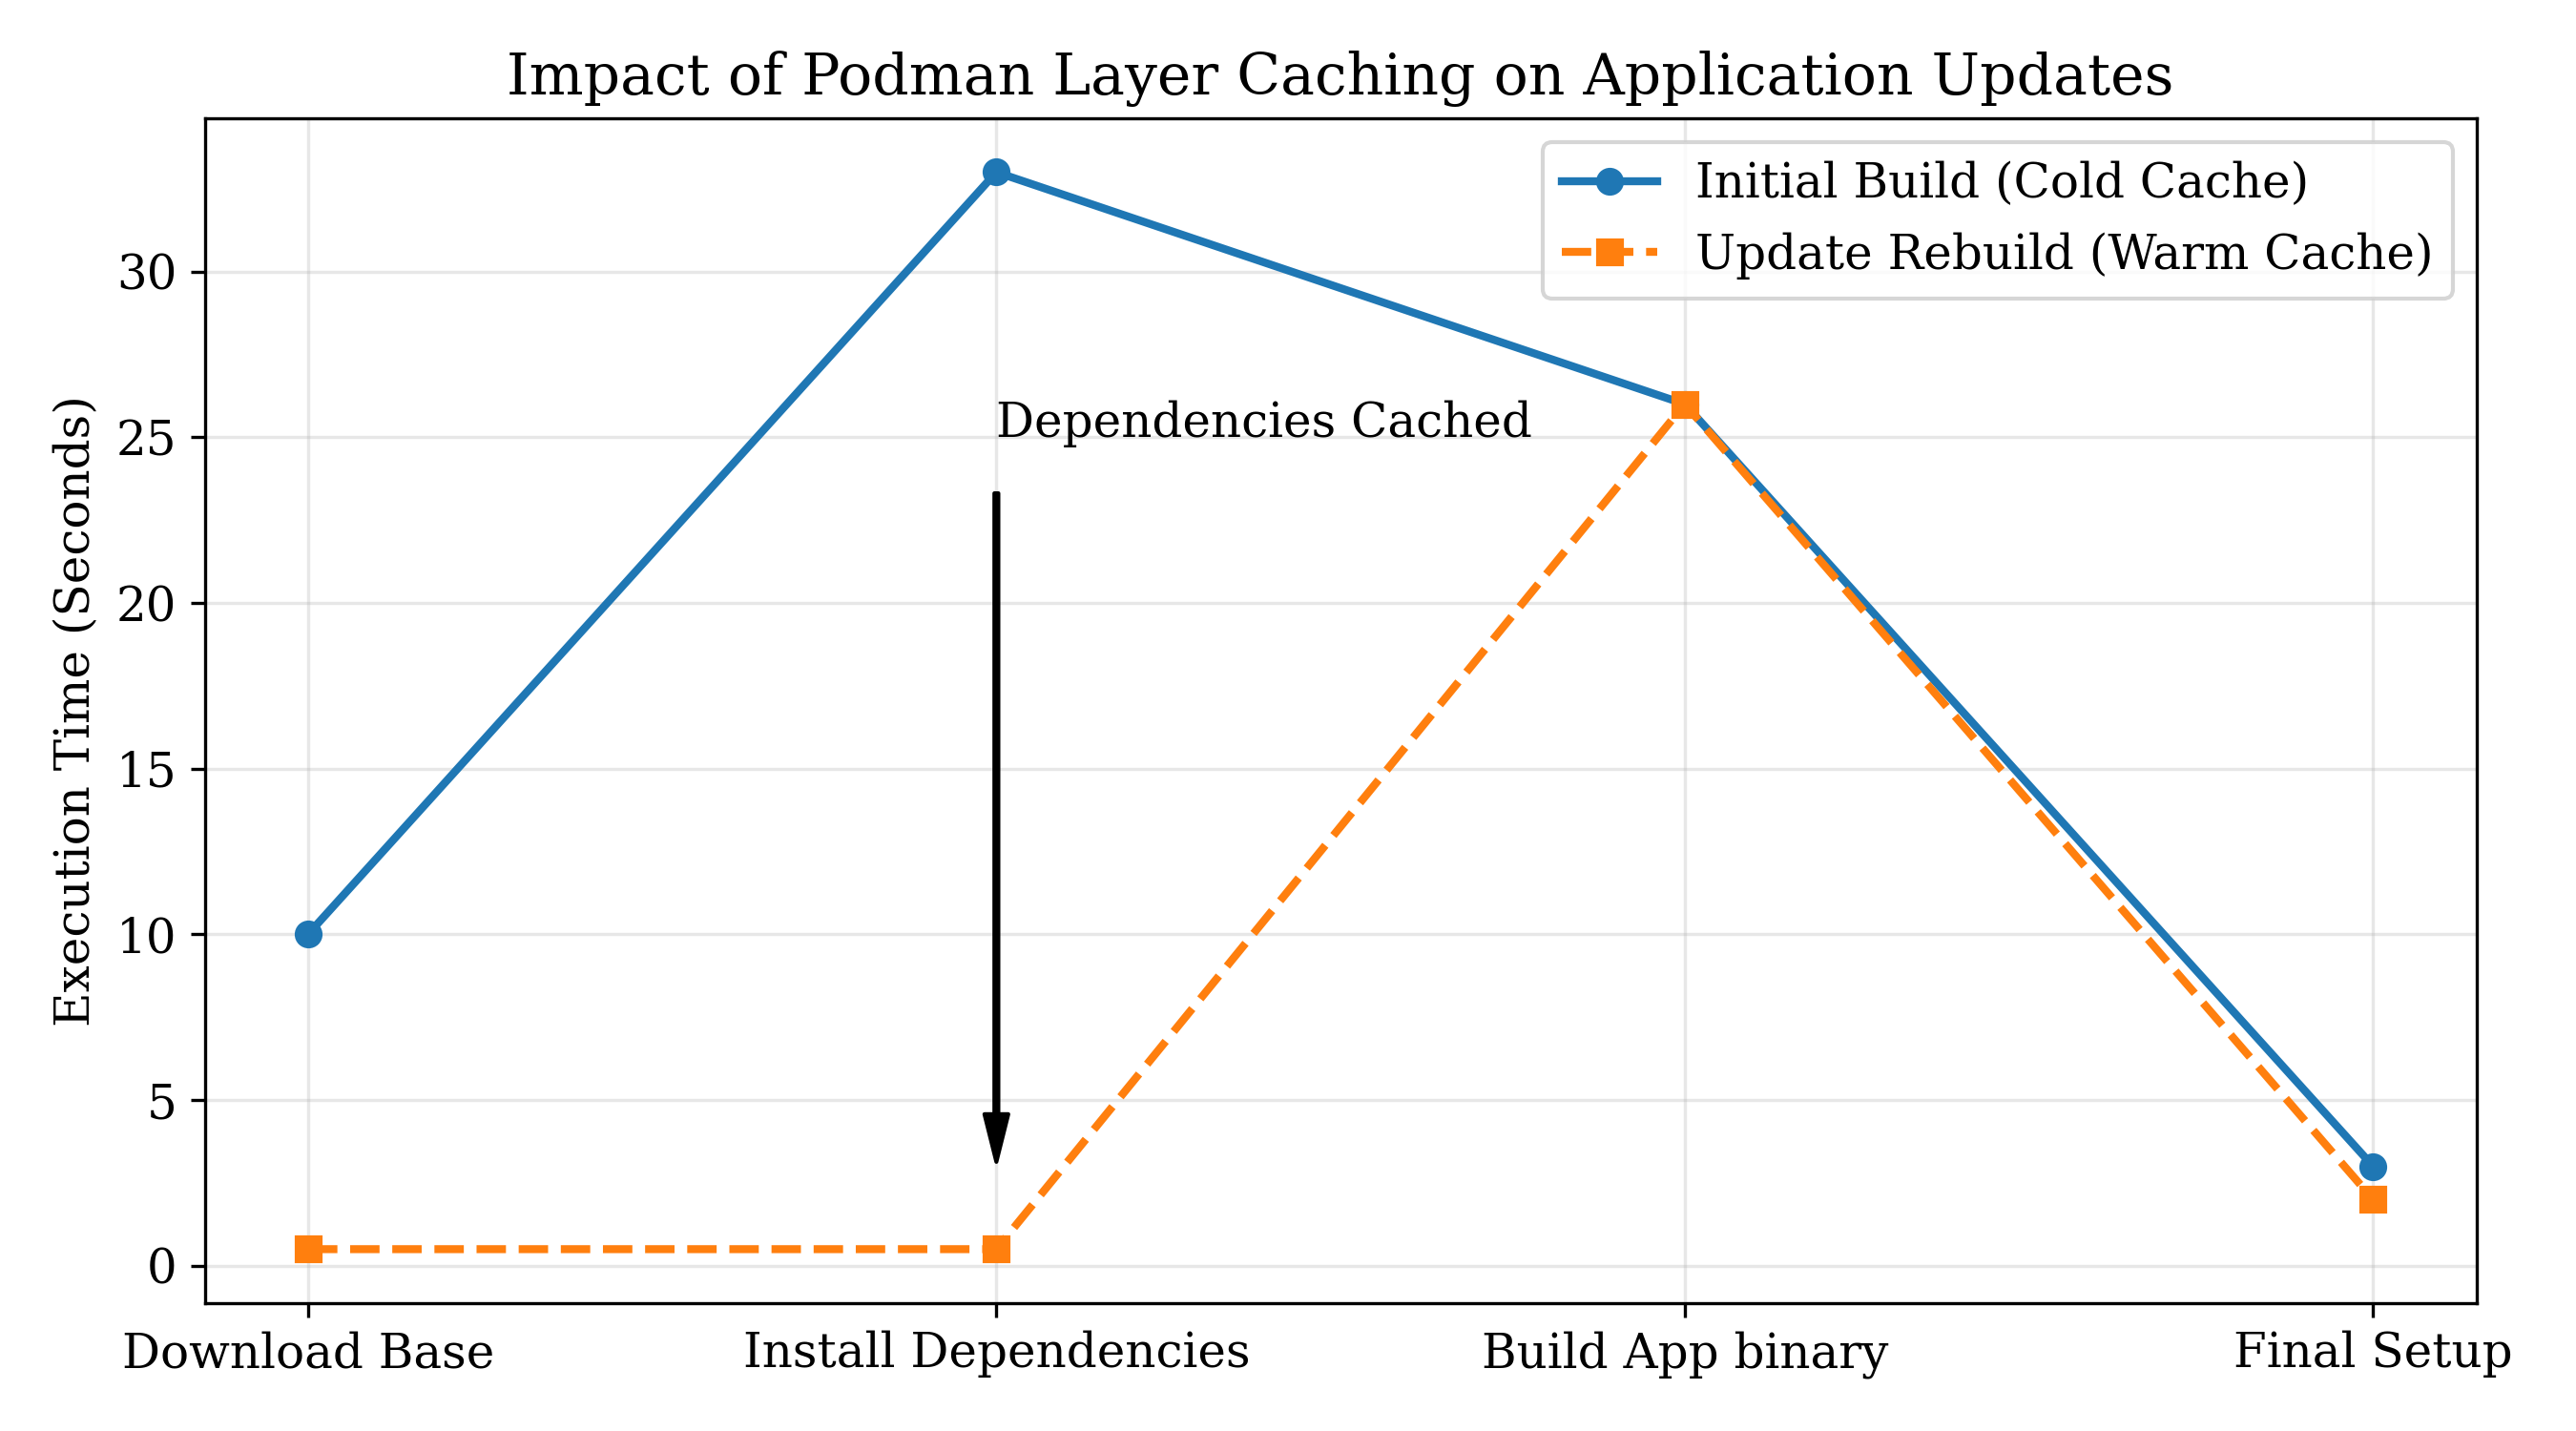
\includegraphics[width=0.6\textwidth]{chart-build-cache}
    \caption{Layer Caching}
    \label{fig:chart-build-cache}
\end{figure}
\newpage
\subsection{Analysis \& Evaluation}
\subsubsection{Analysis of Dependency Mitigation}
The findings shows that containerisation offers a robust solution to the "dependency hell" problem at the host operating system level. By bundling the application and dependencies within the container image, the approach decouples the application's runtime environment from the host distribution's library (e.g., APT, YUM/DNF). This was demonstrated by the ability of the same container images (e.g., the Brave Browser container based on Ubuntu) to run on different host distributions without encountering library conflicts or requiring specific host package installations beyond the container runtime itself.

\subsubsection{Analysis of Superiority}
Compared to traditional methods, this approach eliminates the need for complex dependency algorithms on the host (as discussed in relation to OPIUM\cite{10.1109/ICSE.2007.59}) and avoids the potential for system-wide library version clashes. Unlike universal package formats like Flatpak or Snap, which also provide isolation, the container approach leverages standard container runtime and image formats (OCI-compliant), potentially offering broader compatibility with existing container infrastructure and workflows

\subsubsection{Analysis of Security}
The container isolation utilise Linux kernel features like namespaces and cgroups, offers a significant security advantage compared to installing potentially untrusted applications directly onto the host system. The prototypes demonstrated effective isolation of the application's filesystem and processes. The findings point out that if an attacker can compromise the application inside the container, they might also be able to compromise it if installed natively. The container's isolation aims to confine the damage, preventing easy lateral movement or access to the entire host system, unlike a native application with full user privileges.

\begin{figure}[ht]
    \centering
    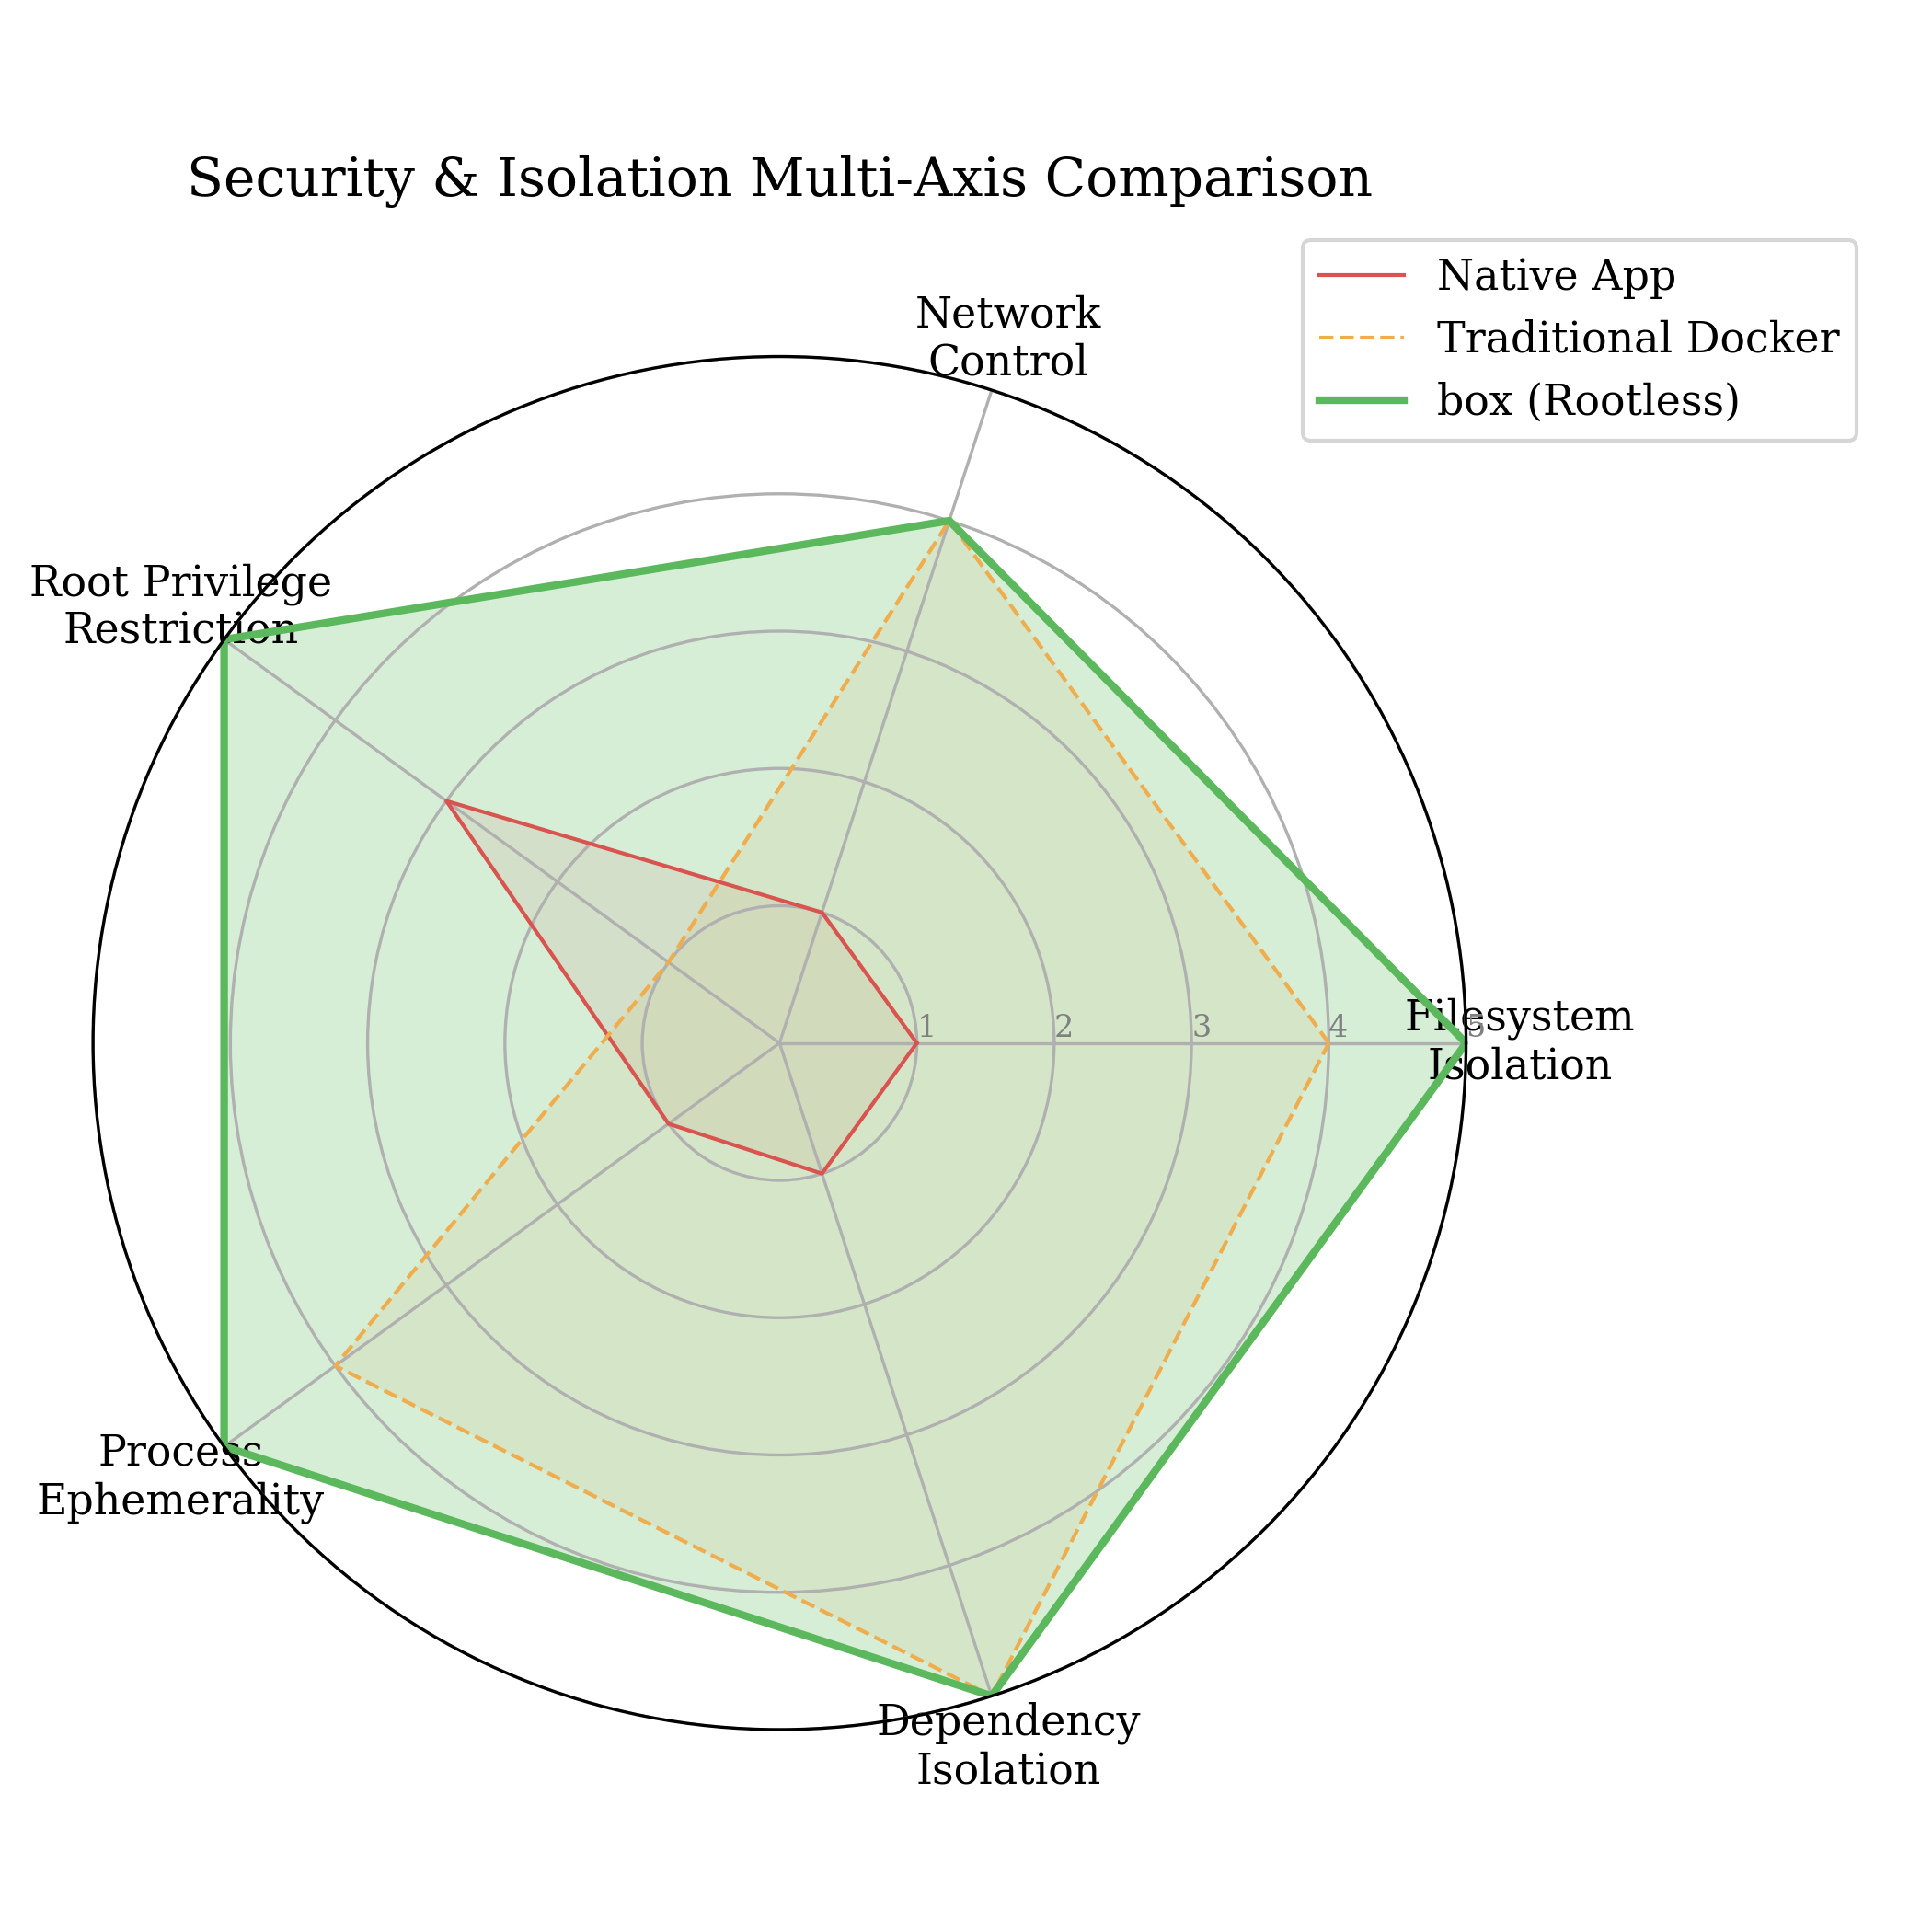
\includegraphics[width=0.4\textwidth]{chart-security-radarchart}
    \caption{Security Radar Comparison}
    \label{fig:chart-security-radarchart}
\end{figure}

\subsubsection{Analysis of Design and End-User Experience}
The prototype development process demonstrate design considerations for building a container-based packaging system for a comprehensive Linux environment. One of the main improvement is the image structure, where multi-stage builds minimise final image size by separating build dependencies from runtime requirements. Managing application dependencies shifts entirely to the Containerfile, requiring developers to accurately define and maintain the required libraries.

\newpage
\subsubsection{Analysis of Performance Metrics}
Startup Time: Figure 12 illustrates the startup time comparison between native installations and containerised executions for the selected applications (Brave Browser, Zoom, Winbox/Wine).
\begin{figure}[ht!]
    \centering
    \subfloat[Brave Browser\label{1a}]{%
    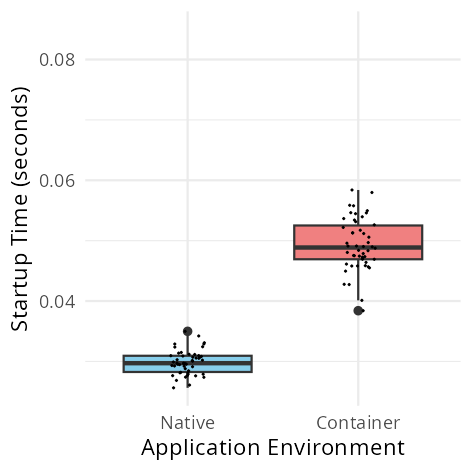
\includegraphics[width=0.3\linewidth]{startup_brave}}
    \hfill
    \subfloat[Zoom\label{1b}]{%
    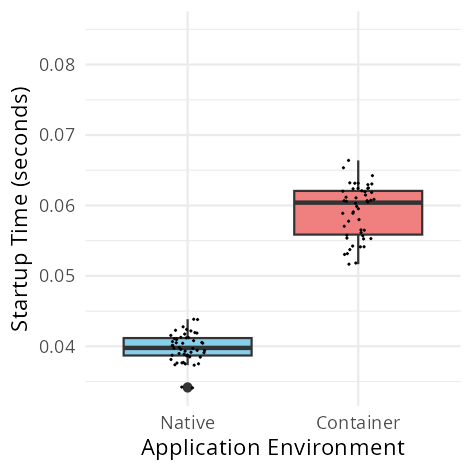
\includegraphics[width=0.3\linewidth]{startup_zoom}}
    \hfill
    \subfloat[Winbox(Wine)\label{1c}]{%
    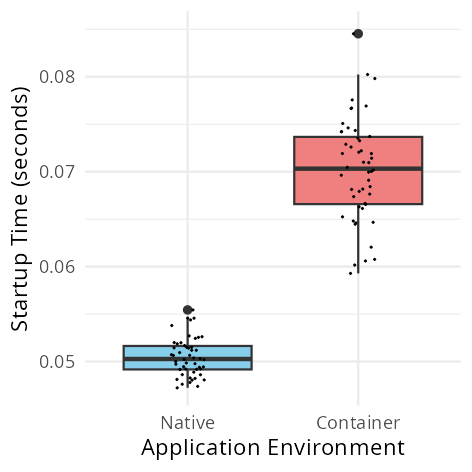
\includegraphics[width=0.3\linewidth]{startup_winbox}}
    \caption{Startup Time Comparison}
\end{figure}

\begin{figure}[ht]
    \centering
    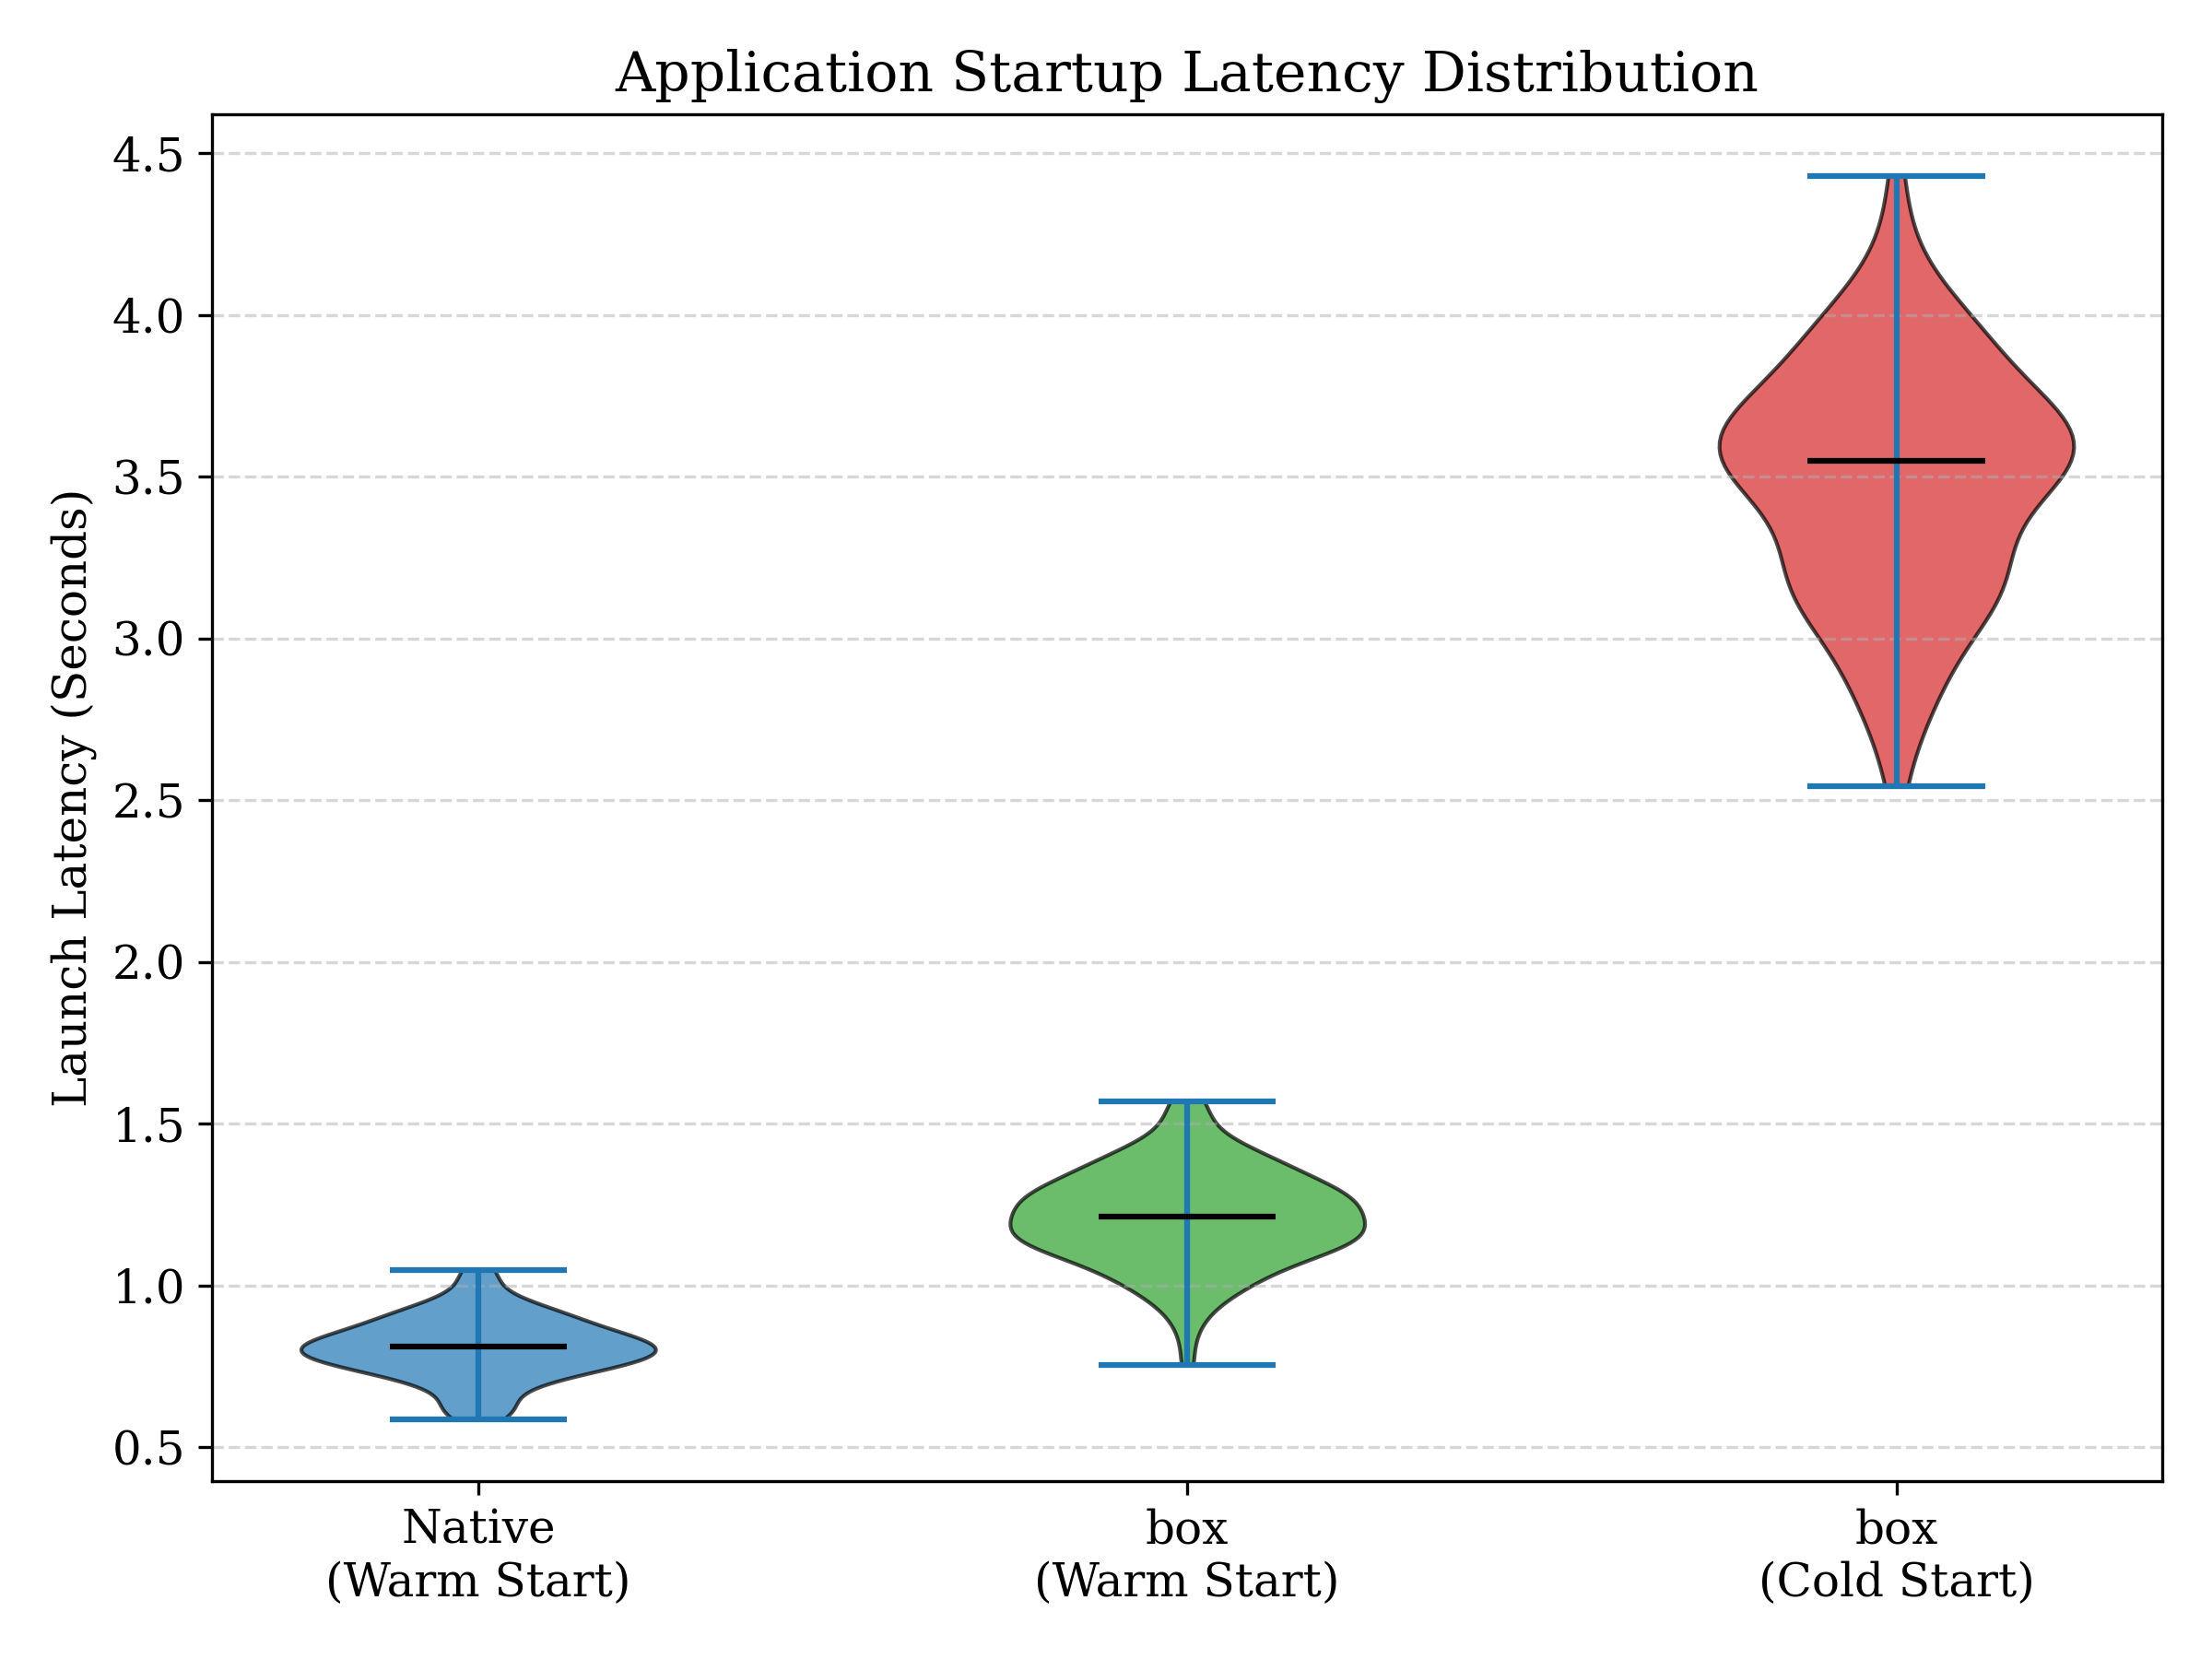
\includegraphics[width=0.6\textwidth]{chart-latency-violinplot}
    \caption{Startup Latency Comparison}
    \label{fig:chart-latency-violinplot}
\end{figure}

The Figure 12 and 13 indicate there are some container overhead delay for each applications. But the difference is only in the sub mill-second region which is not noticeable by end user. During the demonstration, the \code{transient-store} flag is used to lessen the page storage size which might have some effect on the startup time.


\newpage
RAM Usage: Figure 14 and 15 presents the RAM usage comparison between native and containerised applications (Brave Browser, Zoom, Winbox/Wine).

\begin{figure}[ht]
    \centering
    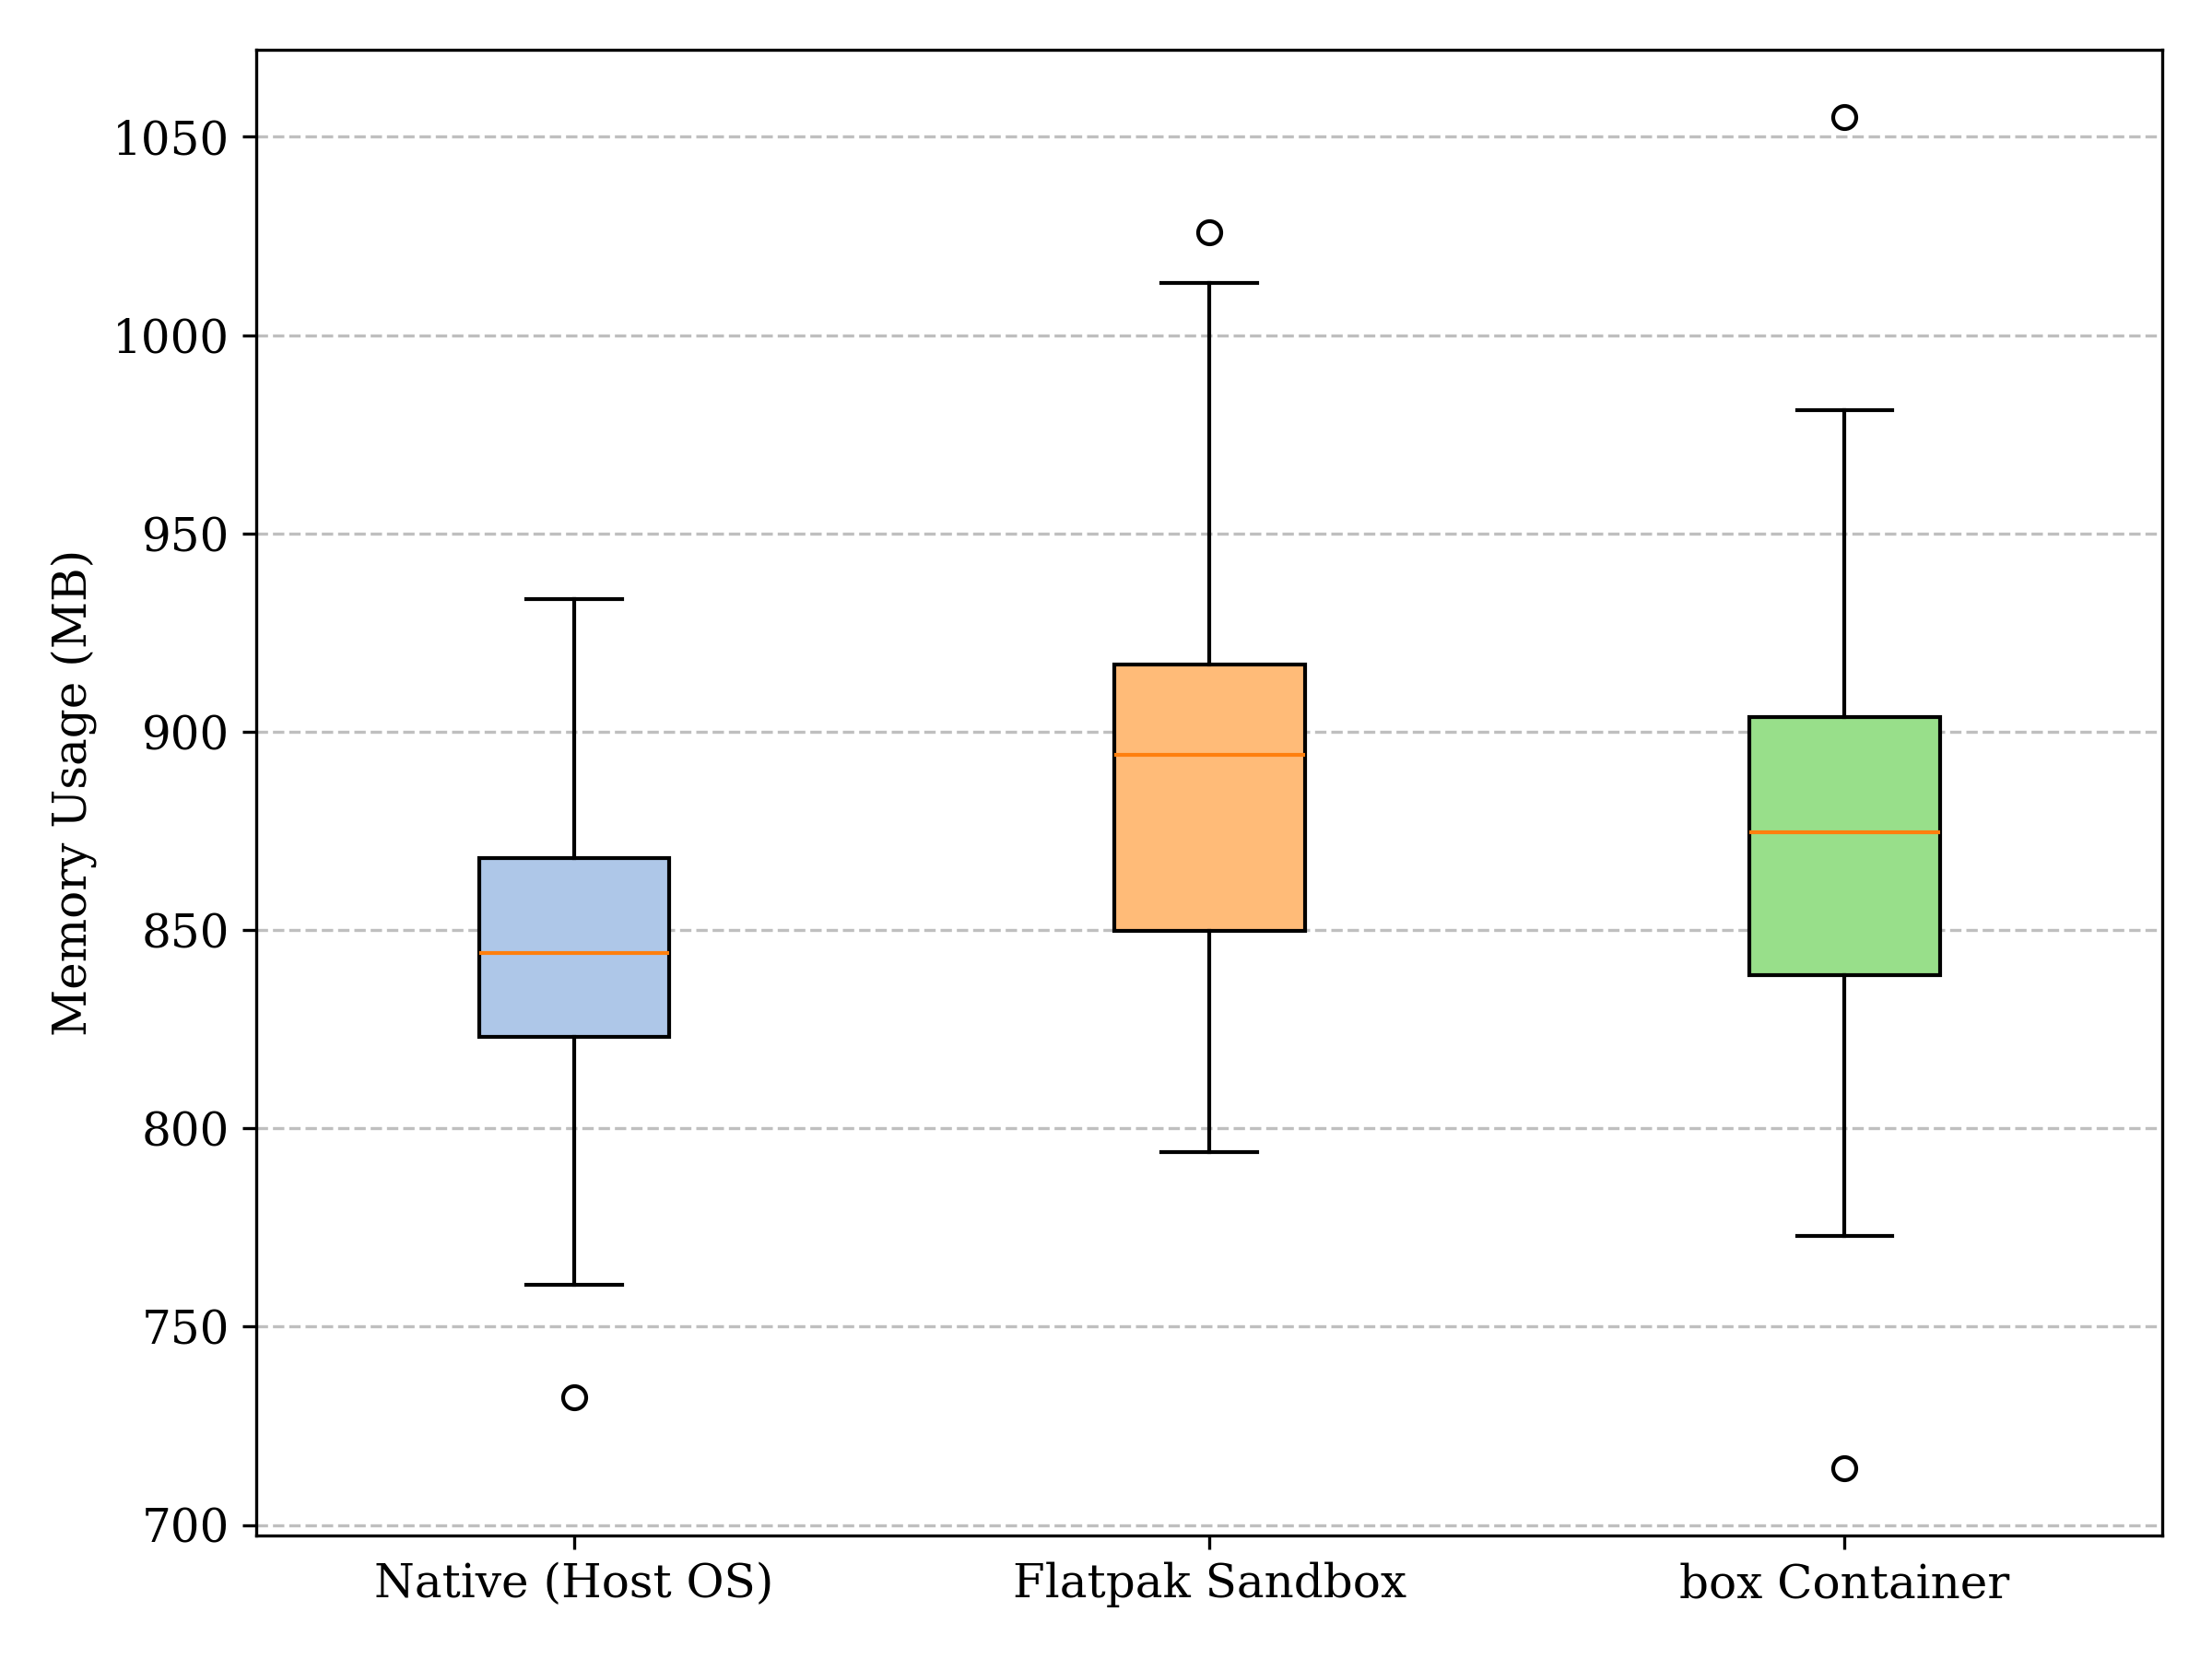
\includegraphics[width=0.6\textwidth]{chart-ram-boxplot}
    \caption{RAM Utilisation Distribution: Web Browser Workload}
    \label{fig:chart-ram-boxplot}
\end{figure}

\begin{figure}[ht!]
    \centering
    \subfloat[Brave Browser\label{2a}]{%
    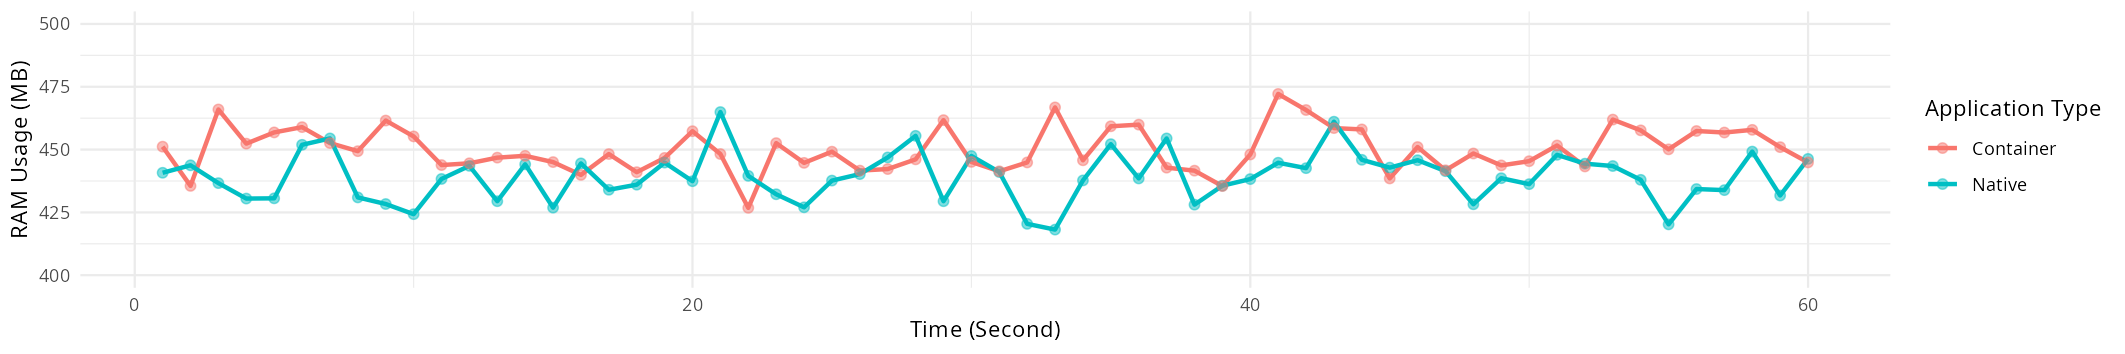
\includegraphics[width=1\linewidth]{ram_brave}}
    \hfill
    \\
    \subfloat[Zoom\label{2b}]{%
    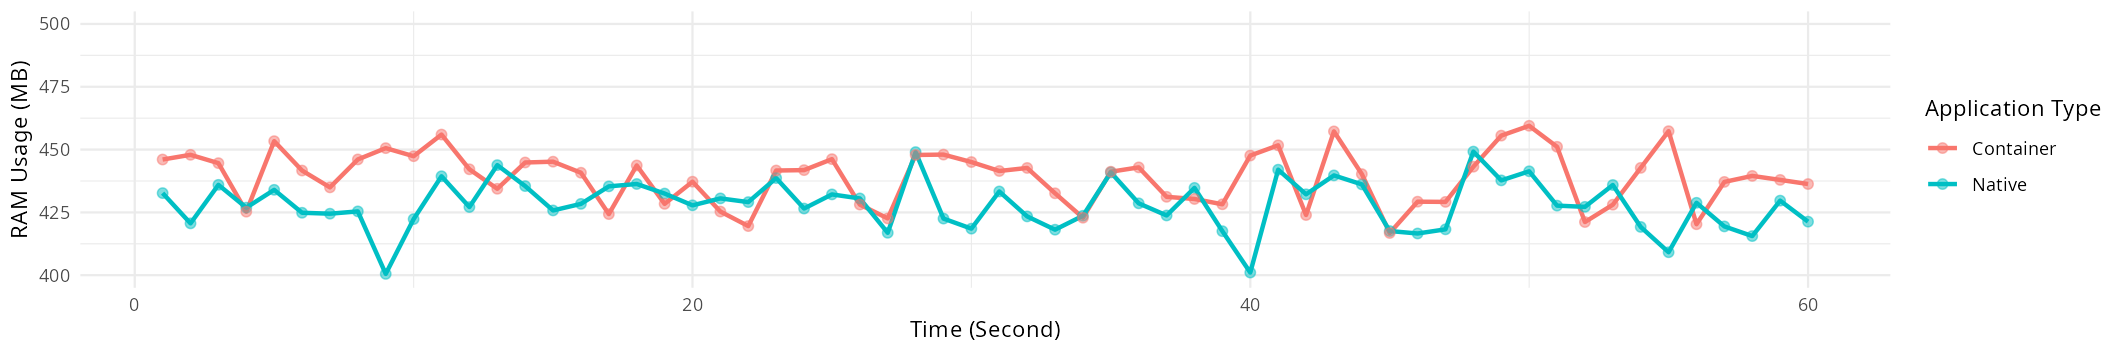
\includegraphics[width=1\linewidth]{ram_zoom}}
    \hfill
    \\
    \subfloat[Winbox(Wine)\label{2c}]{%
    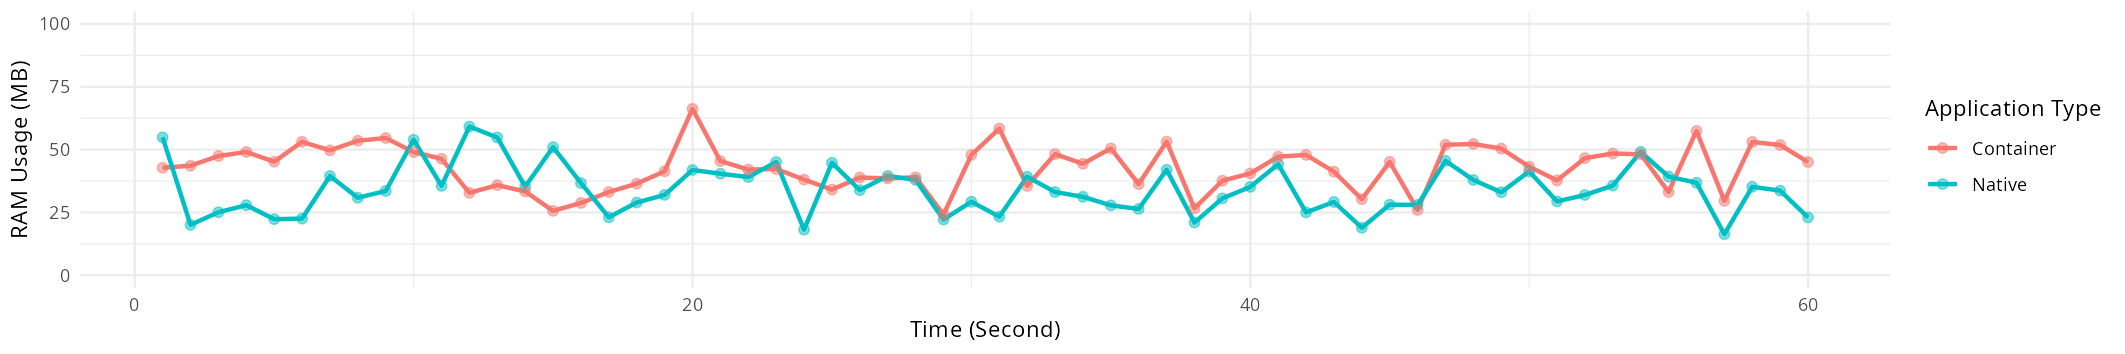
\includegraphics[width=1\linewidth]{ram_winbox}}
    \caption{RAM Usage Comparison}
\end{figure}

Regarding RAM usage, no significant difference was found between the native and container versions of the applications. Sudden dips were observed in the native version but not in the container version, suggesting that the container environment regulates RAM usage to maintain a consistent level.

Overall, the performance analysis suggests that while containerisation offers significant benefits in dependency management and isolation, it may introduce some overhead in startup time and RAM usage compared to highly optimised native installations. These trade-offs must be considered when evaluating the feasibility of a universal container-based system, particularly for performance-sensitive applications or resource-limited environments. The findings align somewhat with the performance trade-offs observed in the Jails vs. Docker study \cite{Ryding_Johansson_2020}, where different container technologies showed strengths in different performance areas.

\newpage
\section{Conclusion}
This research successfully demonstrated that a universal, container-based delivery model can effectively resolve the chronic dependency conflicts and fragmentation inherent in the Linux ecosystem. By moving away from imperative, stateful package managers that frequently induce ``system rot,'' this study proposed and evaluated a ``box'' framework capable of safely encapsulating both command-line and complex Graphical User Interface (GUI) applications. Leveraging the daemonless and rootless architecture of Podman, the framework proved that applications can run with near-native performance while adhering to strict principles of least privilege. 

Our findings validate the effectiveness of encapsulating applications and their required library within a single image. We demonstrated successful running of diverse GUI application across different host environments. For security, we explained the containers inherently offer a layer of isolation compared to native installation using through kernel features. We managed to shared the host resources such as display server, audio and devices where the container isolation layer still provides a border for outer attacks by utilising granular security policies.

From a design perspective, we constructed efficient images, leveraging multi-stage builds to minimise size, and developing robust, abstracted mechanisms for host resource integration. Performance analysis indicated that while containerisation introduces some minimal overhead in application startup time and potentially affects RAM usage consistency compared to highly optimised native installations, these differences were largely imperceptible to users which is suggesting that the performance cost is an acceptable trade-off for the benefits gained in dependency management and isolation.

The implications of these findings are significant for the future of Linux application distribution which can enable developers to target a single, containerised format that runs consistently across virtually any Linux distribution. This could accelerate software availability, simplify maintenance, and provide a more stable user experience by eliminating dependency conflicts.

The findings confirm that shifting the burden of dependency resolution into immutable container images guarantees cross-distribution compatibility and bit-for-bit reproducibility. Crucially, the prototype overcame significant architectural hurdles by dynamically mapping host hardware resources such as display server sockets, audio daemons, and GPU acceleration without compromising the isolation boundary. This paradigm shift not only enhances overall workstation stability but dramatically reduces the ``maintenance tax'' imposed on developers, who are no longer forced to maintain divergent packages for disparate Linux distributions.


\newpage
\section{Future Research}
While this dissertation establishes a functional foundation for a container-native desktop, the rapid evolution of intelligent systems and automated infrastructure presents several critical avenues for future exploration:

\subsection{Autonomous Package Lifecycle Management via LLM Pipelines}
The current framework reduces developer burden, but future iterations should investigate integrating Large Language Models (LLMs) to fully automate package maintenance. An LLM-driven agent could autonomously monitor upstream Git repositories for new software releases, parse changelogs, intelligently resolve dependency updates within the \code{Containerfile}, and trigger the CI/CD compilation pipeline without any human intervention. This self-healing architecture would ensure users receive zero-day updates while entirely eliminating manual maintenance.

\subsection{AI-Driven Security Screening and Threat Detection}
Because container images bundle vast dependency chains, relying purely on static CVE databases is insufficient. Future work should explore deploying AI and machine learning models during the image compilation phase. These models could perform deep dynamic analysis on container images to detect zero-day vulnerabilities, hidden malware, or supply chain poisoning within nested libraries before the image is executed on the host machine.

\subsection{Dynamic Sandbox Permissions Tuning via Machine Learning}
Current container frameworks rely on static permission manifests (e.g., granting permanent access to a webcam or network). Future research could implement behavioural ML models that monitor application telemetry in real-time. The system could dynamically expand or restrict \code{cgroup} resource limits and namespaces based on context, For example, granting microphone access to a sandboxed browser only when the AI detects the user actively initiating a video conferencing session.

\subsection{Deep Integration with Immutable Host Operating Systems}
To maximise the benefits of isolated application containers, further research must explore fusing this framework with emerging read-only, immutable operating systems (such as NixOS or Fedora Silverblue). Running a fully containerised application layer on top of a cryptographically verified, immutable root filesystem would create a practically indestructible and perfectly reproducible workstation paradigm.

\subsection{Cross-Architecture Native Orchestration}
With the increasing prevalence of ARM64 and RISC-V processors in the desktop and mobile space, future iterations must ensure the deployment framework is seamlessly architecture-agnostic. Research should focus on orchestrating multi-architecture manifests that can intelligently fetch, compile, and execute the optimal binary specifically for the host's underlying silicon.

\subsection{Decentralised and P2P Image Registries}
To mitigate the risks of centralised failure or censorship inherent in traditional distribution models (e.g., Docker Hub, Snap Store), future implementations should explore decentralised, peer-to-peer (P2P) image registries utilising protocols like IPFS. This would allow containerised desktop applications to be distributed and verified cryptographically across user networks, increasing ecosystem resilience.

\subsection{AI-Optimised Resource Allocation}
GUI containers inherently introduce minor memory and CPU overheads. Future systems could integrate predictive AI algorithms to analyse user behaviour patterns and intelligently pre-warm containers during high-probability usage windows, or aggressively hibernate inactive containers to a transient disk state, ensuring maximum hardware efficiency.

\newpage
% needed in second column of first page if using \IEEEpubid
%\IEEEpubidadjcol

% \subsubsection{Subsubsection Heading Here}
% Subsubsection text here.


% An example of a floating figure using the graphicx package.
% Note that \label must occur AFTER (or within) \caption.
% For figures, \caption should occur after the \includegraphics.
% Note that IEEEtran v1.7 and later has special internal code that
% is designed to preserve the operation of \label within \caption
% even when the captionsoff option is in effect. However, because
% of issues like this, it may be the safest practice to put all your
% \label just after \caption rather than within \caption{}.
%
% Reminder: the "draftcls" or "draftclsnofoot", not "draft", class
% option should be used if it is desired that the figures are to be
% displayed while in draft mode.
%
%\begin{figure}[!t]
%\centering
%\includegraphics[width=2.5in]{myfigure}
% where an .eps filename suffix will be assumed under latex, 
% and a .pdf suffix will be assumed for pdflatex; or what has been declared
% via \DeclareGraphicsExtensions.
%\caption{Simulation results for the network.}
%\label{fig_sim}
%\end{figure}

% Note that the IEEE typically puts floats only at the top, even when this
% results in a large percentage of a column being occupied by floats.


% An example of a double column floating figure using two subfigures.
% (The subfig.sty package must be loaded for this to work.)
% The subfigure \label commands are set within each subfloat command,
% and the \label for the overall figure must come after \caption.
% \hfil is used as a separator to get equal spacing.
% Watch out that the combined width of all the subfigures on a 
% line do not exceed the text width or a line break will occur.
%
%\begin{figure*}[!t]
%\centering
%\subfloat[Case I]{\includegraphics[width=2.5in]{box}%
%\label{fig_first_case}}
%\hfil
%\subfloat[Case II]{\includegraphics[width=2.5in]{box}%
%\label{fig_second_case}}
%\caption{Simulation results for the network.}
%\label{fig_sim}
%\end{figure*}
%
% Note that often IEEE papers with subfigures do not employ subfigure
% captions (using the optional argument to \subfloat[]), but instead will
% reference/describe all of them (a), (b), etc., within the main caption.
% Be aware that for subfig.sty to generate the (a), (b), etc., subfigure
% labels, the optional argument to \subfloat must be present. If a
% subcaption is not desired, just leave its contents blank,
% e.g., \subfloat[].


% An example of a floating table. Note that, for IEEE style tables, the
% \caption command should come BEFORE the table and, given that table
% captions serve much like titles, are usually capitalized except for words
% such as a, an, and, as, at, but, by, for, in, nor, of, on, or, the, to
% and up, which are usually not capitalized unless they are the first or
% last word of the caption. Table text will default to \footnotesize as
% the IEEE normally uses this smaller font for tables.
% The \label must come after \caption as always.
%
%\begin{table}[!t]
%% increase table row spacing, adjust to taste
%\renewcommand{\arraystretch}{1.3}
% if using array.sty, it might be a good idea to tweak the value of
% \extrarowheight as needed to properly center the text within the cells
%\caption{An Example of a Table}
%\label{table_example}
%\centering
%% Some packages, such as MDW tools, offer better commands for making tables
%% than the plain LaTeX2e tabular which is used here.
%\begin{tabular}{|c||c|}
%\hline
%One & Two\\
%\hline
%Three & Four\\
%\hline
%\end{tabular}
%\end{table}


% Note that the IEEE does not put floats in the very first column
% - or typically anywhere on the first page for that matter. Also,
% in-text middle ("here") positioning is typically not used, but it
% is allowed and encouraged for Computer Society conferences (but
% not Computer Society journals). Most IEEE journals/conferences use
% top floats exclusively. 
% Note that, LaTeX2e, unlike IEEE journals/conferences, places
% footnotes above bottom floats. This can be corrected via the
% \fnbelowfloat command of the stfloats package.









% if have a single appendix:
%\appendix[Proof of the Zonklar Equations]
% or
%\appendix  % for no appendix heading
% do not use \section anymore after \appendix, only \section*
% is possibly needed

% use appendices with more than one appendix
% then use \section to start each appendix
% you must declare a \section before using any
% \subsection or using \label (\appendices by itself
% starts a section numbered zero.)
%


\appendices
\section{Other Containerfile Prototypes and Execution Commands}
Box command shell program

\begin{lstlisting}[language=Bash]
#!/bin/bash

BOX_PATH=$(pwd)

COMPOSE_DIR="${BOX_PATH}/compose"
MOUNT_DIR="${BOX_PATH}/mount"

# GitHub's raw user content layout
REPO_URL="https://raw.githubusercontent.com/peterzam/box/refs/heads/v2"

usage() {
    echo "Box - Manage personal software containers"
    echo "Usage: box <command> [arguments]"
    echo ""
    echo "Commands:"
    echo "  run <program_name>       Run/attach to application via podman-compose"
    echo "  build <program_name>     Build container image using remote GitHub Containerfile"
    echo "                           Options: Default is --no-cache. Pass '--cache' to allow cached layers."
    echo "  install <program_name>   Download the compose manifest configuration file from GitHub into storage"
    echo "  update                   Check running podman image version against GitHub version"
    echo "  uninstall <program_name> Remove the local podman image"
    echo "  box-install [path]       Install this script to ~/.local/bin and lock in the parent [path] (defaults to pwd)"
    exit 1
}

# Ensure at least one argument is provided
if [ $# -lt 1 ]; then
    usage
fi

COMMAND="$1"
shift

case "$COMMAND" in
    run)
        PROGRAM_NAME="$1"
        if [ -z "$PROGRAM_NAME" ]; then
            echo "Error: Please specify a program name to run."
            exit 1
        fi

        COMPOSE_FILE="${COMPOSE_DIR}/${PROGRAM_NAME}/compose.yml"
        if [ ! -f "$COMPOSE_FILE" ]; then
            echo "Error: compose.yml not found at $COMPOSE_FILE. Have you run 'box install ${PROGRAM_NAME}'?"
            exit 1
        fi

        # Looks for any running container whose name contains the program identifier (e.g., box-brave-browser)
        running_container_name=$(podman ps --filter "name=-${PROGRAM_NAME}" --filter "status=running" --format "{{.Names}}" | head -n 1)

        if [ -n "$running_container_name" ]; then
            echo "Container '${running_container_name}' is already running."
            echo "Executing a new session inside the running container..."

            # Parse entrypoint or command arrays out of compose.yml using sed/awk fallbacks
            exec_cmd=$(awk '/^\s*(entrypoint|command):/ && !found {
                            found = 1; 
                            match($0, /^\s*/); indent = RLENGTH; # Remember the indentation level
                            sub(/^\s*(entrypoint|command):\s*/, ""); # Strip the key prefix
                            print; next;
                            }
                            found {
                                match($0, /^\s*/);
                                if (RLENGTH > indent || $0 ~ /^\s*$/) {
                                  sub(/^\s*-\s*/, ""); # Strip YAML list dashes (-) if they exist
                                  print;
                                } else { exit } # Stop as soon as indentation goes back to normal
                              }
                            ' "$COMPOSE_FILE" | tr -d '"'\''[]>|')
            if [ -z "$exec_cmd" ]; then
                if podman exec "$running_container_name" which bash >/dev/null 2>&1; then
                    exec_cmd="bash"
                else
                    exec_cmd="sh"
                fi
            fi

            # Execute terminal directly using the verified container name string
            podman exec -it "$running_container_name" $exec_cmd
        else
            # Pre-create the program-specific mount subdirectory within the new centralized mount folder
            mkdir -p "$MOUNT_DIR"

            echo "Starting a fresh '${PROGRAM_NAME}' container stack detached (-d)..."
            echo "Compose Context: $COMPOSE_FILE"
            echo "Mount Context:   $MOUNT_DIR"
            
            # Map BOX_MOUNT to the consolidated mount path for the compose layer
            PUID=$(id -u) PGID=$(id -g) BOX_MOUNT="$MOUNT_DIR" podman-compose -f "$COMPOSE_FILE" up -d
        fi
        ;;

    build)
        PROGRAM_NAME="$1"
        OPTIONAL_FLAG="$2"
        if [ -z "$PROGRAM_NAME" ]; then
            echo "Error: Please specify a program name to build."
            exit 1
        fi

        remote_containerfile="${REPO_URL}/${PROGRAM_NAME}/Containerfile"
        echo "Fetching and parsing version metadata from remote GitHub Containerfile..."
        
        # Temp fetch top comments to safely track version tag configurations
        version=$(curl -sL --max-time 5 "$remote_containerfile" | head -n 5 | grep -i '^#\s*version:' | sed -E 's/^#\s*version:\s*//I' | xargs)

        # Evaluate cache flags natively passed downstream
        CACHE_ARG="--no-cache"
        if [ "$OPTIONAL_FLAG" = "--cache" ]; then
            echo "Flag '--cache' detected. Building container using layer caching mechanics..."
            CACHE_ARG=""
        else
            echo "Building cleanly via --no-cache context defaults..."
        fi

        echo "Building container image using remote asset context stream..."
        image_name="peterzam/box-${PROGRAM_NAME}"
        
        # Pull and compile via direct HTTP Context stream without requiring local file storage clones
        podman build $CACHE_ARG -t "${image_name}:latest" -f "$remote_containerfile" "https://github.com/peterzam/box.git#main:${PROGRAM_NAME}"
        
        if [ -n "$version" ]; then
            echo "Tagging image with version: ${version}"
            podman tag "${image_name}:latest" "${image_name}:${version}"
        else
            echo "Warning: No '# version:' comment found in remote GitHub Containerfile. Skipping version tagging."
        fi
        ;;

    install)
        PROGRAM_NAME="$1"
        if [ -z "$PROGRAM_NAME" ]; then
            echo "Error: Please specify a program name to install."
            exit 1
        fi

        TARGET_DIR="${COMPOSE_DIR}/${PROGRAM_NAME}"
        echo "Creating target app directory inside consolidated compose registry: $TARGET_DIR..."
        mkdir -p "$TARGET_DIR"

        remote_compose_url="${REPO_URL}/${PROGRAM_NAME}/compose.yml"
        echo "Downloading compose layout configuration from: $remote_compose_url"
        
        curl -sL --max-time 10 "$remote_compose_url" -o "${TARGET_DIR}/compose.yml"

        if [ -s "${TARGET_DIR}/compose.yml" ]; then
            echo "Configuration manifest saved successfully to: ${TARGET_DIR}/compose.yml"
            echo "    You can now run: box build ${PROGRAM_NAME} followed by box run ${PROGRAM_NAME}"
        else
            echo "Error: Failed to fetch valid content from GitHub endpoint. Removing blank profile context."
            rm -rf "$TARGET_DIR"
            exit 1
        fi
        ;;

    update)
        echo "Checking local Podman image versions against GitHub..."
        echo "========================================================"
        
        if [ ! -d "$COMPOSE_DIR" ]; then
            echo "Error: The consolidated compose directory does not exist: $COMPOSE_DIR"
            exit 1
        fi

        for dir in "${COMPOSE_DIR}"/*/; do
            [ -d "$dir" ] || continue
            prog=$(basename "$dir")
            
            image_name="localhost/peterzam/box-${prog}"
            
            local_version=$(podman image inspect "$image_name" --format '{{join .RepoTags ", "}}' 2>/dev/null \
                | tr ',' '\n' \
                | grep -v 'latest' \
                | sed -E "s|.*${image_name}:||" \
                | xargs)
            
            if [ -z "$local_version" ]; then
                local_version="unknown"
            fi
            
            remote_url="${REPO_URL}/${prog}/Containerfile"
            remote_version=$(curl -sL --max-time 5 "$remote_url" | head -n 5 | grep -i '^#\s*version:' | sed -E 's/^#\s*version:\s*//I' | xargs)
            
            if [ -z "$remote_version" ]; then
                echo "[-] ${prog}: Local Image [${local_version}] | GitHub version could not be fetched."
            elif [ "$local_version" != "$remote_version" ]; then
                echo "[!] ${prog}: UPDATE DETECTED! Local Image: [${local_version}] -> GitHub File: [${remote_version}]"
                echo "    To upgrade, run: box build ${prog}"
            else
                echo "${prog}: Up to date (Image Version: ${local_version})"
            fi
        done
        ;;

    uninstall)
        PROGRAM_NAME="$1"
        if [ -z "$PROGRAM_NAME" ]; then
            echo "Error: Please specify a program name to uninstall."
            exit 1
        fi

        image_name="peterzam/box-${PROGRAM_NAME}"
        echo "Uninstalling: Cleaning up local podman images matching ${image_name}..."
        
        podman rmi $(podman images -q "${image_name}") 2>/dev/null || podman rmi "${image_name}:latest" 2>/dev/null

        if [ $? -eq 0 ]; then
            echo "Images associated with '${PROGRAM_NAME}' removed successfully."
        else
            echo "[-] No local podman images found for '${PROGRAM_NAME}' or failed to delete."
        fi
        ;;

    box-install)
        TARGET_BOX_PATH="$1"
        if [ -z "$TARGET_BOX_PATH" ]; then
            TARGET_BOX_PATH="$(pwd)"
        fi
        
        TARGET_BOX_PATH=$(realpath "$TARGET_BOX_PATH")

        INSTALL_DIR="$HOME/.local/bin"
        mkdir -p "$INSTALL_DIR"
        
        cp "$0" "$INSTALL_DIR/box"
        
        # Lock in the shared parent path folder context
        sed -i "s|^BOX_PATH=.*|BOX_PATH=\"${TARGET_BOX_PATH}\"|" "$INSTALL_DIR/box"
        chmod +x "$INSTALL_DIR/box"
        
        # Automatically structure the parent directory with its core internal workspaces
        mkdir -p "${TARGET_BOX_PATH}/compose" "${TARGET_BOX_PATH}/mount"
        
        echo "Successfully installed 'box' executable tool to $INSTALL_DIR/box"
        echo "Centralized parent directory:  ${TARGET_BOX_PATH}"
        echo "Compose workspace subfolder:   ${TARGET_BOX_PATH}/compose"
        echo "Central mounts subfolder:      ${TARGET_BOX_PATH}/mount"
        echo "Make sure '$INSTALL_DIR' is configured inside your local environment's PATH."
        ;;

    *)
        echo "Unknown command: $COMMAND"
        usage
        ;;
esac
\end{lstlisting}

\begin{figure}[ht]
    \centering
    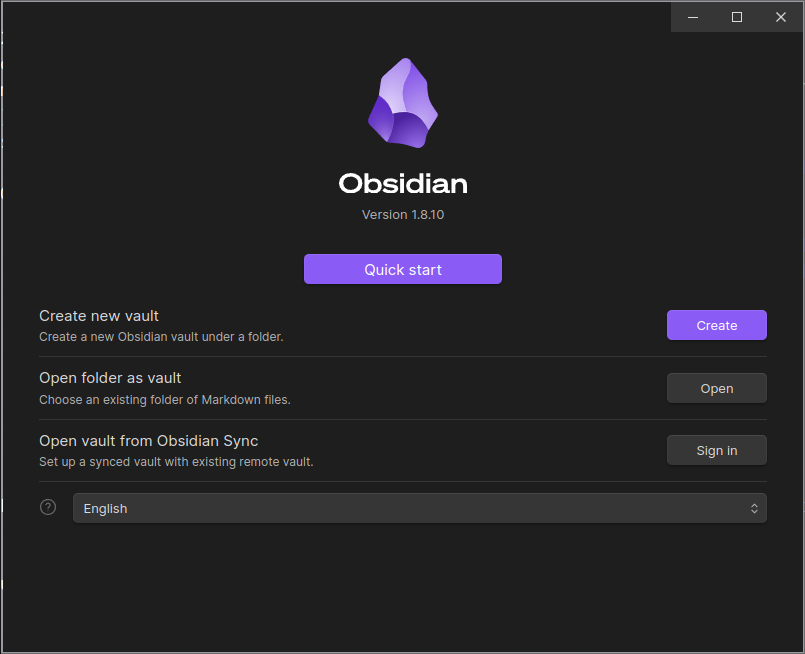
\includegraphics[width=0.8\textwidth]{proto-obsidian.png}
    \caption{Obsidian Note Taking App in Container}
    \label{fig:proto-obsidian}
\end{figure}

\begin{figure}[ht]
    \centering
    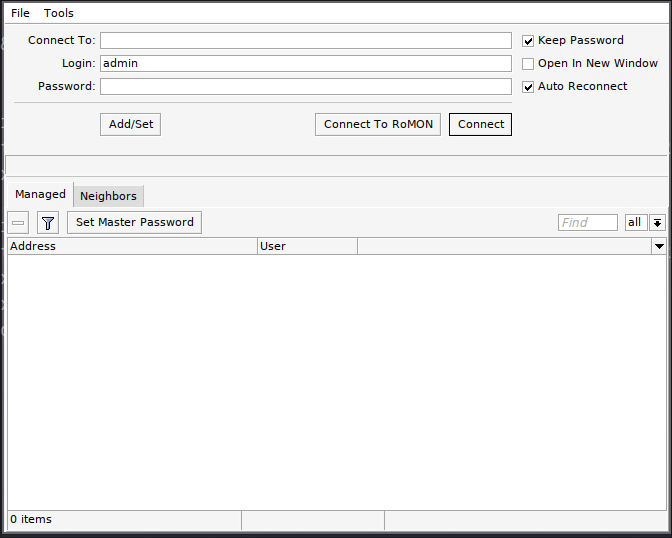
\includegraphics[width=0.8\textwidth]{proto-winbox.png}
    \caption{Windows App - Winbox in Container}
    \label{fig:proto-winbox}
\end{figure}

\begin{figure}[ht]
    \centering
    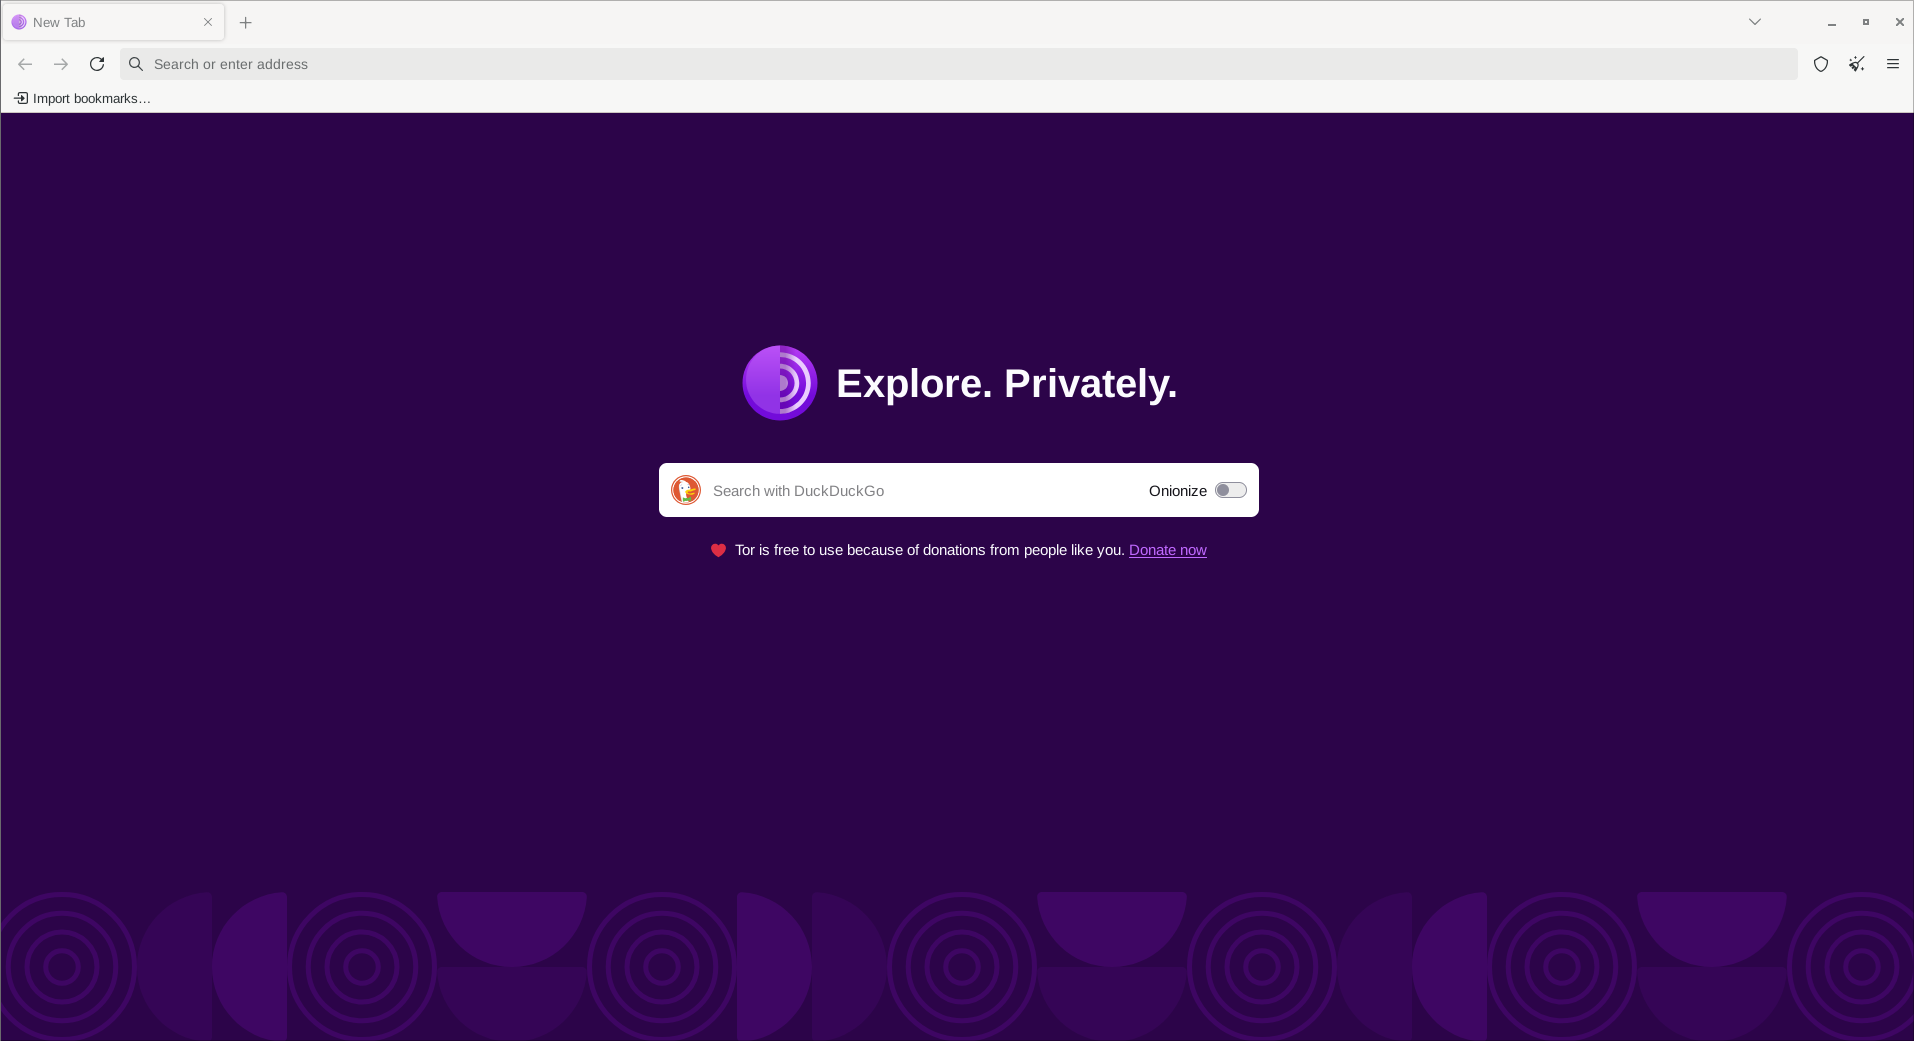
\includegraphics[width=0.8\textwidth]{proto-tor.png}
    \caption{Tor Browser in Container}
    \label{fig:proto-tor}
\end{figure}

\section{Benchmarking and Survey}
\subsubsection{Benchmarking Methodology Details} 
Exact commands used for measurement (e.g., time -p <command>, htop for peak RAM, specific perf commands).
Used tools: time, htop, perf, grafana, prometheus



\subsection{Podman System Detail}
\begin{lstlisting}[language=Bash]
host:
  arch: amd64
  buildahVersion: 1.40.1
  cgroupControllers:
  - cpu
  - memory
  - pids
  cgroupManager: systemd
  cgroupVersion: v2
  conmon:
    package: conmon-1:2.1.13-1
    path: /usr/bin/conmon
    version: 'conmon version 2.1.13, commit: 82de887596ed8ee6d9b2ee85e4f167f307bb569b'
  cpuUtilization:
    idlePercent: 90.4
    systemPercent: 1.1
    userPercent: 8.5
  cpus: 16
  databaseBackend: sqlite
  distribution:
    distribution: arch
    version: unknown
  eventLogger: journald
  freeLocks: 2047
  hostname: arch
  idMappings:
    gidmap:
    - container_id: 0
      host_id: 1000
      size: 1
    - container_id: 1
      host_id: 100000
      size: 65536
    uidmap:
    - container_id: 0
      host_id: 1000
      size: 1
    - container_id: 1
      host_id: 100000
      size: 65536
  kernel: 6.14.10-arch1-1
  linkmode: dynamic
  logDriver: journald
  memFree: 768892928
  memTotal: 15518031872
  networkBackend: netavark
  networkBackendInfo:
    backend: netavark
    dns:
      package: aardvark-dns-1.15.0-1
      path: /usr/lib/podman/aardvark-dns
      version: aardvark-dns 1.15.0
    package: netavark-1.15.2-1
    path: /usr/lib/podman/netavark
    version: netavark 1.15.2
  ociRuntime:
    name: crun
    package: crun-1.21-1
    path: /usr/bin/crun
    version: |-
      crun version 1.21
      commit: 10269840aa07fb7e6b7e1acff6198692d8ff5c88
      rundir: /run/user/1000/crun
      spec: 1.0.0
      +SYSTEMD +SELINUX +APPARMOR +CAP +SECCOMP +EBPF +CRIU +YAJL
  os: linux
  pasta:
    executable: /usr/bin/pasta
    package: passt-2025_06_06.754c6d7-1
    version: |
      pasta 2025_06_06.754c6d7
      Copyright Red Hat
      GNU General Public License, version 2 or later
        <https://www.gnu.org/licenses/old-licenses/gpl-2.0.html>
      This is free software: you are free to change and redistribute it.
      There is NO WARRANTY, to the extent permitted by law.
  remoteSocket:
    exists: true
    path: /run/user/1000/podman/podman.sock
  rootlessNetworkCmd: pasta
  security:
    apparmorEnabled: false
    capabilities: CAP_CHOWN,CAP_DAC_OVERRIDE,CAP_FOWNER,CAP_FSETID,CAP_KILL,CAP_NET_BIND_SERVICE,CAP_SETFCAP,CAP_SETGID,CAP_SETPCAP,CAP_SETUID,CAP_SYS_CHROOT
    rootless: true
    seccompEnabled: true
    seccompProfilePath: /etc/containers/seccomp.json
    selinuxEnabled: false
  serviceIsRemote: false
  slirp4netns:
    executable: ""
    package: ""
    version: ""
  swapFree: 12883607552
  swapTotal: 12884897792
  uptime: 3h 45m 29.00s (Approximately 0.12 days)
  variant: ""
plugins:
  authorization: null
  log:
  - k8s-file
  - none
  - passthrough
  - journald
  network:
  - bridge
  - macvlan
  - ipvlan
  volume:
  - local
registries: {}
store:
  configFile: /home/p/.config/containers/storage.conf
  containerStore:
    number: 1
    paused: 0
    running: 1
    stopped: 0
  graphDriverName: overlay
  graphOptions: {}
  graphRoot: /home/p/.local/share/containers/storage
  graphRootAllocated: 511017222144
  graphRootUsed: 207637196800
  graphStatus:
    Backing Filesystem: btrfs
    Native Overlay Diff: "true"
    Supports d_type: "true"
    Supports shifting: "false"
    Supports volatile: "true"
    Using metacopy: "false"
  imageCopyTmpDir: /var/tmp
  imageStore:
    number: 1
  runRoot: /run/user/1000/containers
  transientStore: false
  volumePath: /home/p/.local/share/containers/storage/volumes
version:
  APIVersion: 5.5.1
  Built: 1749464740
  BuiltTime: Mon Jun  9 10:25:40 2025
  GitCommit: 850db76dd78a0641eddb9ee19ee6f60d2c59bcfa
  GoVersion: go1.24.4
  Os: linux
  OsArch: linux/amd64
  Version: 5.5.1
\end{lstlisting}

\subsection{Survey Questions}

\begin{itemize}

\item What is your experience level with Linux? (Beginner, Intermediate, Advanced)"

\item What is your experience level with containerisation technologies (Docker/Podman)? (None, Basic, Intermediate, Advanced)

\item On a scale of 1 to 5, how noticeable was the difference in startup time between the native and containerised versions of Brave Browser? (1=Not noticeable at all, 5=Very noticeable)

\item Did you perceive any difference in responsiveness, smoothness or performance when using the containerised application compared to the native one? Please elaborate.

\item What was your general impression of using applications delivered via containers? (Positive, Negative, Neutral, Why?)

\end{itemize}

\subsection{Alternative Approaches and Technologies Considered}
\begin{itemize}
    \item Other Container Runtimes/Technologies
    \begin{itemize}
        \item LXC/LXD: more system-level virtualisation, less emphasis on application packaging portability.
        \item systemd-nspawn: capabilities and limitations for GUI application isolation.
    \end{itemize}
    \item Alternative GUI Integration Methods
    \begin{itemize}
        \item VNC/SPICE servers within the container: adds overhead, less native.
        \item SSH X forwarding: performance, setup complexity.
        \item Nested Wayland compositors: Complicated and not stable.
    \end{itemize}
\end{itemize}

\subsection{Glossary of Technical Terms and Acronyms}
\begin{itemize}
    \item OCI: Open Container Initiative
    \item cgroups: Control Groups
    \item Namespaces: Linux kernel feature for resource isolation (PID, NET, MNT, UTS, IPC, USER)
    \item Wayland: A display server protocol
    \item X11: The X Window System, a display server protocol
    \item PulseAudio: A sound server for POSIX and Windows systems
    \item PipeWire: A server for handling audio, video streams, and hardware on Linux
    \item Seccomp: Secure Computing Mode
    \item AppArmor/SELinux: Linux security modules
    \item DLL Hell: Dynamic Link Library conflict issue on Windows
    \item Dependency Hell: Software dependency conflict issue on Linux
    \item APT: Advanced Package Tool (Debian/Ubuntu)
    \item YUM/DNF: Yellowdog Updater, Modified / Dandified YUM (Red Hat/Fedora)
    \item AUR: Arch User Repository
    \item CLI: Command Line Interface
    \item GUI: Graphical User Interface
    \item PoC: Proof of Concept
    \item UX: User Experience
    \item DX: Developer Experience
    \item Containerd: Industry-standard container runtime
    \item libpod: Library for Podman, providing container management functionality
\end{itemize}
% you can choose not to have a title for an appendix
% if you want by leaving the argument blank
% \section{}
% Appendix two text goes here.


% use section* for acknowledgment
\newpage
\section*{Acknowledgment}


The author wish to thank Dr. Jian Yu\cite{P-Jian}, Associate Professor, for his guidance and supervision throughout this research. 

The author would also like to thank the following projects for their knowledge and support.

\begin{itemize}
\item x.org\cite{xorg}
\item zoom.com\cite{zoom}
\item brave.com\cite{brave}
\item winehq.org\cite{winehq}
\item kernel.org\cite{kernelorg}
\item ubuntu.com\cite{ubuntu}
\item obsidian.md\cite{obsidian}
\item flatpak.org\cite{flatpak}
\item appimage.org\cite{appimage}
\item apparmor.net\cite{apparmor}
\item overleaf.com\cite{overleaf}
\item mikrotik.com\cite{mikrotik}
\item snapcraft.io\cite{snapcraft}
\item r-project.org\cite{rproject}
\item torproject.org\cite{torproject}
\item alpinelinux.org\cite{alpinelinux}
\item github.com/docker\cite{docker_github}
\item fedoraproject.org\cite{fedora}
\item latex-project.org\cite{latexproject}
\item github.com/containers\cite{containers_github}
\item ggplot2.tidyverse.org\cite{ggplot2}
\item wayland.freedesktop.org\cite{wayland}
\item github.com/peterzam/box\cite{peterzambox}
\item freedesktop.org/wiki/Software/PulseAudio\cite{pulseaudio_wiki}
\end{itemize}

Thanks are also extended to the survey respondents and the authors of the works cited in this paper.
\newpage
% Can use something like this to put references on a page
% by themselves when using endfloat and the captionsoff option.
\ifCLASSOPTIONcaptionsoff
  \newpage
\fi



% trigger a \newpage just before the given reference
% number - used to balance the columns on the last page
% adjust value as needed - may need to be readjusted if
% the document is modified later
%\IEEEtriggeratref{8}
% The "triggered" command can be changed if desired:
%\IEEEtriggercmd{\enlargethispage{-5in}}

% references section

% can use a bibliography generated by BibTeX as a .bbl file
% BibTeX documentation can be easily obtained at:
% http://mirror.ctan.org/biblio/bibtex/contrib/doc/
% The IEEEtran BibTeX style support page is at:
% http://www.michaelshell.org/tex/ieeetran/bibtex/
\bibliographystyle{IEEEtran}
\bibliography{IEEEabrv,references}
% argument is your BibTeX string definitions and bibliography database(s)
%\bibliography{IEEEabrv,../bib/paper}
%
% <OR> manually copy in the resultant .bbl file
% set second argument of \begin to the number of references
% (used to reserve space for the reference number labels box)
% \begin{thebibliography}{1}

% \bibitem{IEEEhowto:kopka}
%H.~Kopka and P.~W. Daly, \emph{A Guide to \LaTeX}, 3rd~ed.\hskip 1em plus
%  0.5em minus 0.4em\relax Harlow, England: Addison-Wesley, 1999.

%\end{thebibliography}

% biography section
% 
% If you have an EPS/PDF photo (graphicx package needed) extra braces are
% needed around the contents of the optional argument to biography to prevent
% the LaTeX parser from getting confused when it sees the complicated
% \includegraphics command within an optional argument. (You could create
% your own custom macro containing the \includegraphics command to make things
% simpler here.)
%\begin{IEEEbiography}[{\includegraphics[width=1in,height=1.25in,clip,keepaspectratio]{mshell}}]{Michael Shell}
% or if you just want to reserve a space for a photo:

% \begin{IEEEbiography}{Michael Shell}
% Biography text here.
% \end{IEEEbiography}

% if you will not have a photo at all:
% \begin{IEEEbiographynophoto}{John Doe}
% Biography text here.
% \end{IEEEbiographynophoto}

% insert where needed to balance the two columns on the last page with
% biographies
%\newpage

% \begin{IEEEbiographynophoto}{Jane Doe}
% Biography text here.
% \end{IEEEbiographynophoto}

% You can push biographies down or up by placing
% a \vfill before or after them. The appropriate
% use of \vfill depends on what kind of text is
% on the last page and whether or not the columns
% are being equalized.

%\vfill

% Can be used to pull up biographies so that the bottom of the last one
% is flush with the other column.
%\enlargethispage{-5in}



% that's all folks
\end{document}